\chapter{Merging as Fair Collective Choice}\label{ch:5}
In this chapter we look at merging as a collective decision mechanism
akin to an election, whose goal is to aggregate information originating 
with different agents.
As mentioned in Section \ref{sec:3-merging},
our approach in this work sees merging as a task 
whose role is not so much to find the true answer, but 
rather to find a compromise between the different opinions 
of the participans.
In this, our main purpose is to make sure that the aggregation process 
is \emph{fair} towards the agents involved, in all the various ways 
that fairness can be conceived of:
to this end, we look to the social choice literature,
which contains an arsenal of properties that have been used 
to ensure fairness of voting rules
\cite{Zwicker16,BaumeisterR16},
and seek to apply these properties to the context of merging.
This involves, first of all, refitting the main intuitions
to the context of merging, which is not always straightforward,
and seeing to what extent existing merging operators satisfy 
the newly minted properties.
In some cases, we take cues from the social choice literature 
even to design new merging operators, tailored specifically to these properties.

What makes the appropriation of classical social choice properties 
challenging, in certain cases, are the differences between merging 
operators and classical voting rules.
Though merging operators can be seen as social choice functions,
as mentioned in Section \ref{sec:3-merging},
they differ from standard voting rules as analyzed in social choice theory,
in that they do not require agents to rank all possible alternatives.
What agents provide to a merging operator are formulas:
if we identify formulas with their models, 
and think of the models as candidates up for election, 
then, under postulate $\ppm{2}$, merging operators 
can be seen as social choice functions that require agents 
to submit only their top preferences.
Nonetheless, the representation result in Section \ref{sec:3-merging}
shows how, under certain assumptions, 
preferences creep in even when not explicitly provided.

\begin{xmpl}{$\#$OscarsSoFossilized, again}{5-merging-motivation}
	We return to the four Academy members from Example \ref{ex:1-merging-motivation} 
	trying to decide the nominees for the category of Best Director.
	The three options (Alma Har'el, Bong Joon Ho and C\'eline Sciamma) 
	are represented by propositional atoms $a$, $b$ and $c$.
	The opinions of the four Academy members are represented by the formulas
	$\phi_1 = a\land b$,
	$\phi_2 = a\land (b\lor c)$,
	$\phi_3 = \lnot a\land b \land \lnot c$.
	and
	$\phi_4 = \lnot a \land\lnot b\land c$,
	gathered in the profile $\P=(\phi_1,\phi_2,\phi_3,\phi_4)$.
	The list has to be whittled down to two,
	i.e., there is a constraint 
	$\mu=(a\land b\land \lnot c)\lor (a\land\lnot b\land c)\lor(\lnot a\land b\land c)$,
	with $[\mu]=\{ab,bc,ac\}$,
	that needs to be satisfied.
	A merging operator $\me$ satisfying postulates $\ppm{0-8}$ 
	delivers a propositional formula $\me_\mu(\P)$ that, 
	among other things, satisfies $\mu$.
	What is more, according to Theorem \ref{thm:3-merging-repr}
	we know that every formula $\phi_{i}\in \P$ 
	induces a total preorder $\le_{\phi_i}$ on outcomes.

	Thus, merging the formulas in $\P$ can be seen as an election
	where the voters are the Academy members (i.e., the agents supplying the formulas),
	the candidates are the viable nominee lineups (i.e., the models of $\mu$)
	and the voting rule is the merging operator $\me$.
	In this context, the agents' beliefs can be seen as
	encoding their top options:
	thus, Academy member $1$'s opinion $\phi_1$ has as models the interpretations 
	$ab$ and $abc$, which, according to postulate $\ppm{2}$, 
	are the Academy member's most preferred outcomes in their 
	corresponding preference order $\le_{\phi_1}$.
	In Section \ref{sec:3-merging} we have also seen that 
	distances between interpretations and aggregation functions 
	can be used to generate a total preorder based on the opinions 
	provided by the agents, i.e., it need not be assumed that agents 
	hold the preference order is their `heads', or have to explicitly 
	provide them.
\end{xmpl}

Thus, though belief merging operators and voting rules 
share a common goal and methodology, 
the parameters of a belief merging operator are subtly 
different from those of a classical voting rule,
with the closest match in social choice being 
models of combinatorial voting based on completion principles 
\cite{LangX16}.
Nonetheless, we believe that the wealth of insights 
accumulated by social choice theory 
on voting methods can be brought to bear on merging operators.

The main thrust of this chapter lies in a series of properties 
meant to capture various aspects of fairness in the merging process.
We present these properties as postulates that 
a merging operator $\me$ is expected to satisfy,
and intend them as additions to 
the standard merging postulates:
our purpose, to be clear, is not to suggest that 
postulates $\ppm{0-8}$ are wrong, or that they have 
to be replaced; the postulates we look at are meant 
to stand alongside the existing postulates and complement them.
As such, our contribution aims to extend the standard characterization
of merging operators 
by offering more fine-grained criteria for their evaluation.
We group the properties according to their character, 
and offer discussions on the behavior they are intended to model.
In the case of each new property, we study its 
relationship with the core postulates $\ppm{0-8}$.
When a property is not guaranteed by these postulates, 
we investigate which of the standard operators 
%(summation-based, $\gmax$, $\gmin$)
satisfy the property,
give relevant counter-examples, 
and provide model-based representation results for the most prominent of these properties.

% The motivation for proposing new properties is the same as the motivation behind the original postulates: 
% we are interested in merging operators that are fair and that respond in expected ways to changes in the input, 
% and we want general principles that capture these properties. 
% Our claim is that there are many ways of making these intuitions precise, 
% some of which go beyond the core postulates $\ppm{0-8}$. 





























\section{Insensitivity to syntax}\label{sec:5-syntax}
The properties in this section are grouped around the idea that the outcome
of a merging task should depend only on the semantic content of the information provided
and not on details about how the information is written down,
perceived here as extraneous.
More concretely, the idea is that aspects 
of the syntax of the elements of merging 
should not affect the result of the merging process.
This is an intuition that is already familiar to us,
since the standard postulate $\ppm{3}$ already expresses 
a form of insensitivity to syntax. 
However, there are more nuances to this 
principle than $\ppm{3}$ manages to capture.

Before presenting the actual properties we have in mind, 
we must become acquainted with some notions, some of them 
new and some of them old. 
The first notions describe ways of swapping things around 
in a profile.
Recall that a permutation $\perm$ of the set of agents $N=\{1,\dots,n\}$
is a bijection $\perm\colon N\rightarrow N$.
If $\P=(\phi_i)_{1\le i \le n}$ is a propositional profile 
and $\perm$ is a permutation of $N$,  
the \emph{permutation $\perm$ of $\P$} is defined as the profile 
$\P=(\phi_{\perm(i)})_{1\le i \le n}$,
i.e., the profile obtained by changing the order 
of the formulas in $\P$ in accordance with $\perm$. 
A renaming $\rnm$ of the set $\Atoms$ of atoms 
is a permutation of the atoms in $\Atoms$,
and is familiar from Section \ref{sec:4-postulates}. 
We extend it now to profiles, 
and say that if $\rnm$ is a renaming of $\Atoms$ and 
$\P=(\phi_i)_{1\le i \le n}$ is a propositional profile,
\emph{the renaming $\rnm(\P)$ of $\P$} is the profile 
$\P=(\rnm(\phi_i))_{1\le i \le n}$.

The next notion describe ways of getting rid of certain types 
of information, which, for some reason, may become redundant.
If $p$ and $q$ are atoms in $\Atoms$ and $\phi$ is a propositional formula,
the \emph{bundling $\phi^{p\bndl q}$ of $p$ into $q$ in $\phi$} 
is the formula obtained by replacing every occurrence of $p$ in $\phi_i$ with $q$.
If $\P=(\phi_1,\dots,\phi_n)$ is a propositional profile,
the \emph{bundling $\P^{p\bndl q}$ of $p$ into $q$ in $\P$}
is the profile $\P^{p\bndl q}=(\phi^{p\bndl q}_1,\dots,\phi^{p\bndl q}_n)$,
obtained by replacing every occurrence of $p$ in $\phi_i$ with $q$, 
for every $\phi\in \P$.

We can now introduce the actual postulates.
They are intended to apply 
for any profile $\P$, 
propositional formula $\mu$,
permutation $\perm$ of $\mathbb{N}$,
renaming $\rnm$ of the atoms in $\Atoms$ and
atoms $p$ and $q$:

\begin{description}
	\item[($\ppm{\ANON}$)] $\me_\mu(\P) \equiv \me_\mu(\perm(\P))$.
	\item[($\ppm{\NEUT}$)] $\rnm(\me_\mu(\P)) \equiv \me_{\rnm(\mu)}(\rnm(\P))$.
	\item[($\ppm{\BNDL}$)] $\me_{\mu \land (p \leftrightarrow q)}(\P) \models \me_{\mu^{p\bndl q}}(\P^{p\bndl q})$.
\end{description}

Postulate $\ppm{\ANON}$, where `$\ANON$' stands for \emph{anonymity}, requires that 
the result of a merging task is invariant under permutations of the formulas in 
a profile, 
and is an analogue of the anonymity property often encountered in voting \cite{BaumeisterR16,Zwicker16}.
It is a desirable property if, as is usually the case, 
it is felt that the result should not depend on the order
in which agents submit their opinions: 
it should not matter to the aggregation process what an agent's
social security number is, or at what time in the day the agent submits its preferences.
An $\L^{n}$-merging operator $\me$ is \emph{anonymous} if it satisfies postulates $\ppm{\ANON}$.

Postulate $\ppm{\NEUT}$, where `$\NEUT$' stands for \emph{neutrality},
says that the result of a merging task is invariant 
under permutations of the atoms.
Postulate $\ppm{\NEUT}$ is a close analogue 
of the revision postulate $\ppr{\NEUT}$ from Section \ref{sec:4-postulates}.
In a voting scenario neutrality requires that if two candidates are swapped in all votes, 
then they are also swapped in the result.
Its purpose is to ensure that all candidates are treated equally in the determination of the winners, 
i.e., their names do not matter.
Since in the context of merging candidates are outcomes
and outcomes are uniquely identified by the atoms that are true in them,
we apply the neutrality property at the level of the atoms.
An $\L^{n}$-merging operator $\me$ is \emph{neutral} if 
it satisfies postulates $\ppm{\NEUT}$.


The last postulate in this section is $\ppm{\BNDL}$, where `$\BNDL$'
stands for \emph{bundling}. 
Though it has no direct equivalent in the voting literature,
postulate $\ppm{\BNDL}$ bears some resemblance to a property of voting rules 
called \emph{Independence of clones} \cite{BaumeisterR16},
and is motivated by a similar intuition:
alternatives that are in some sense redundant should not skew the vote in their favour.  
The intuition behind this property is best illustrated by an example.

\begin{xmpl}{Bundling}{5-bundling}
	In the scenario described in Example \ref{ex:5-merging-motivation},
	with four Academy members trying to decide who will be the \emph{Best Director} nominees,
	a very unlikely thing happens: Alma Har'el and Bong Joon Ho are discovered to be
	the same person.  
	The show must go on, of course, 
	but unfortunately this revelation comes after the Academy members have submitted their opinions,
	and it is too late to go back and have them redo their evaluation.
	What is known for sure, however, is that any distinction between Alma Har'el and Bong Joon Ho
	in the decision process has to be erased. 
\end{xmpl}

Example \ref{ex:5-bundling} provides a motivation for the bundling postulate $\ppm{\BNDL}$: 
at some point in the modeling process, variables $p$ and $q$, 
which hitherto had been thought to stand for different things,
are discovered to encode the same concept.
% The responsible action is to incorporate this new information in the merging outcome.
%These redundant variables can, of course, lead to undesired effects when the formulas are merged.
One way to incorporate this information 
in the merging process is by `bundling' $p$ into $q$ in the formulas and in the constraint:
as it were, cutting every occurrence of $p$ and pasting $q$ where $p$ had been.
This is quite a laborious and invasive operation on the formulas, 
which might be infeasible if access to the formulas is limited or if the formulas are provided 
by the agents just in time for the merging process.
Another way is to add the equivalence $p \leftrightarrow q$ directly to the constraint
and enforce that $p$ and $q$ are tied up together in perpetuity.
Postulate $\ppm{\BNDL}$ explores the relationship between these two operations 
and requires that all solutions of the latter operation are also solutions of the former.

\begin{xmpl}{Anonymity, neutrality and bundling}{5-insensitivity-syntax}
	For the profile 	
	$\P=(\phi_1,\phi_2,\phi_3,\phi_4)$
	with
	$\phi_1 = a\land b$,
	$\phi_2 = a\land (b\lor c)$,
	$\phi_3 = \lnot a\land b \land \lnot c$
	and
	$\phi_4 = \lnot a \land\lnot b\land c$,
	the constraint $\mu=(a\land b\land \lnot c)\lor (a\land\lnot b\land c)\lor(\lnot a\land b\land c)$,
	the merging operator $\me^{\hamming,\:\min}$
	and a permutation $\perm$ such that $\perm(1)=2$, $\perm(2)=3$, $\perm(3)=4$ and $\perm(4)=1$,
	we obtain that $[\me^{\hamming,\:\ssum}_\mu(\P)]=\{ab,bc\}$ and:
	\begin{align*}
		[\me^{\hamming,\:\ssum}_\mu(\P)] &= [\me^{\hamming,\:\ssum}_\mu(\phi_1,\phi_{2},\phi_{3},\phi_4)]\\ 
		&= [\me^{\hamming,\:\ssum}_\mu(\phi_2,\phi_{3},\phi_{4},\phi_1)]\\
		&= [\me^{\hamming,\:\ssum}_\mu(\phi_{\perm(1)},\phi_{\perm(2)},\phi_{\perm(3)},\phi_{\perm(4)})] 
		= [\me^{\hamming,\:\ssum}_\mu(\perm(\P))].	
	\end{align*}
	This is consistent with postulate $\ppm{\ANON}$.

	If $\rnm$ is a renaming of $\Atoms$ such that 
	$\rnm(a)=b$, $\rnm(b)=c$ and $\rnm(c)=a$, 
	we have that
	$\rnm(\phi_1) = b\land c$,
	$\rnm(\phi_2) = b\land (c\lor a)$,
	$\rnm(\phi_3) = \lnot b\land c \land \lnot a$,
	$\rnm(\phi_4) = \lnot b \land\lnot c\land a$,
	$\rnm(\mu)\equiv\mu$,
	and $[\me^{\hamming,\:\ssum}_{\rnm(\mu)}(\rnm(\P))]=\{bc,ca\}=[\rnm(\me^{\hamming,\:\ssum}_\mu(\P))]$,
	which is consistent with postulate $\ppm{\NEUT}$.

	If we bundle $b$ into $a$, we have that
	$\phi^{b\bndl a}_{1} = a\land a$,
	$\phi^{b\bndl b}_{2} = a\land (a\lor c)$,
	$\phi^{b\bndl a}_{3} = \lnot a\land a\land \lnot c$, 
	$\phi^{b\bndl a}_{4} = \lnot a\land \lnot a\land c$
	and
	$\mu^{b\bndl a}=(a\land a\land \lnot c)\lor (a\land\lnot a\land c)\lor(\lnot a\land a\land c)$.
	We obtain that 
	$[\me^{\hamming,\:\ssum}_{\mu^{b\bndl a}}(\P^{b\bndl a})]=\{ab\}$.	
	On the other hand, note that 
	$[\mu\land(a\leftrightarrow b)]=\{ab\}$ and thus
	$[\me^{\hamming,\:\ssum}_{\mu\land(a\leftrightarrow b)}(\P)]=\{ab\}$.
	This result is consistent with postulate $\ppm{\BNDL}$.
\end{xmpl}

To understand the postulates just introduced it is, of course, 
useful to see how they work on the semantic level,
i.e., to understand what kind of properties need to hold 
for the preorders in an $\L^n$-assignment $\as$ on interpretations
that represents the merging operator.
Thus, if $\as$ is an $\L^n$-assignment on interpretations 
that satisfies properties $\oom{1-9}$ and $\rnm$ is a renaming on $\Atoms$,
the following properties turn out to be relevant,
when applying for any propositional profile $\P$ and 
interpretations $w_1$ and $w_2$:

\begin{description}
	\item[($\oom{\ANON}$)] If $w_1 \le_{\P} w_2$, then $w_1 \le_{\perm(\P)} w_2$.	
	\item[($\oom{\NEUT}$)] If $w_1 \le_{\P} w_2$, then $\rnm(w_1) \le_{\rnm(\P)} \rnm(w_2)$.
\end{description}

Property $\oom{\ANON}$ says that if $w_1$ is considered at least as good as $w_2$ 
in the preorder corresponding to $\P$, then this situation should be preserved in the 
preorder corresponding to $\perm(\P)$.
Since the inverse $\perm^{-1}$ of $\perm$ is also a permutation,
property $\oom{\ANON}$ implies, of course, that 
$\le_{\P}=\le_{\perm(\P)}$,
i.e., the preorder $\le_{\P}$ assigned to profile $\P$ 
is identical to the preorder $\le_{\perm(\P)}$ assigned to 
the profile $\perm(\P)$, obtained by permuting the formulas in $\P$ according to $\perm$.
Property $\oom{\NEUT}$ expresses a similar property, but with 
respect to renamings, and likewise implies that $\le_{\P} = \le_{\rnm(\P)}$,
i.e., the preorder $\le_{\P}$ associated to a profile $\P$ 
is identical to the preorder $\le_{\rnm(\P)}$ assigned to the profile $\rnm(\P)$,
obtained by renaming $\P$.
An $\L^n$-assignment $\as$ on interpretations 
is \emph{anonymous} if it satisfies property $\oom{\ANON}$
and \emph{neutral} if it satisfies property $\oom{\NEUT}$.


% \begin{lemma}\label{lemma:5-neut-2}
% 	If $\phi_1$ and $\phi_2$ are any propositional formulas,
% 	it holds that if $\phi_1 \equiv \phi_2$, then $\tau(\phi_1) \equiv \tau(\phi_2)$.
% \end{lemma}
% \begin{prf*}{}{}%
% 	Since $[\phi_1]=[\phi_2]$, it follows that $\tau([\phi_1])= \tau([\phi_2])$. 
% 	This, then, implies that $[\tau(\phi_1)] = [\tau(\phi_2)]$, 
% 	hence $\tau(\phi_1) \equiv \tau(\phi_2)$.
% \end{prf*}

% \begin{lemma}\label{lemma:5-neut-3}
% 	If $\me$ is a merging operator that satisfies postulates $\ppm{0-8}$
% 	and $\as$ is an $\L^n$-assignment on interpretations that represents it and that satisfies property $\oom{\NEUT}$,
% 	then $\tau(\me_{\mu}(\P)) \equiv \me_{\tau(\mu)}(\tau(\P))$, for any transposition $\tau$. 
% \end{lemma}
% \begin{prf*}{}{}%
% 	We have to show that $[\tau(\me_{\mu}(\P))] = [\me_{\tau(\mu)}(\tau(\P))]$, 
% 	or, equivalently, that $\tau(\min_{\le_\P}[\mu])=\min_{\le_{\tau(\P)}}\tau([\mu])$. 
% 	We do so by double inclusion.
% 	First, take $w\in\min_{\le_\P}[\mu]$ and 
% 	an arbitrary $\tau(w')\in\tau([\mu])$, with $w'\in[\mu]$.
% 	Then $\tau(w) \in \tau([\mu])$ and $w\le_\P w'$.
% 	Since the assignment satisfies property $\oom{\NEUT}$, 
% 	it follows that $\tau(w)\le_{\tau(E]}\tau(w')$.
% 	Thus $\tau(w) \in \min_{\le_{\tau(\P)}}\tau([\mu])$.
	
% 	Second, take $\tau(w)\in \min_{\le_{\tau(\P)}}\tau([\mu])$ 
% 	and an arbitrary $w'\in[\mu]$.
% 	We have that $\tau(w)\le_{\tau(\P)}\tau(w')$ and, 
% 	since the assignment satisfies property $\oom{\NEUT}$, 
% 	this implies that $\tau(\tau(w))\le_{\tau(\tau(\P))}\tau(\tau(w'))$.
% 	But $\tau$ is a transposition, hence $\tau(\tau(w))=w$, for any interpretation $w$.
% 	Thus, we obtain that $w\le_\P w'$, which implies that 
% 	$w\in\min_{\le_\P}[\mu]$, and therefore $\tau(w)\in \tau(\min_{\le_\P}[\mu])$.
% \end{prf*}

Intuitively, we would expect that postulates $\ppm{\ANON}$ and $\ppm{\NEUT}$ map onto 
properties $\oom{\ANON}$ and $\oom{\NEUT}$, 
i.e., that anonymous and neutral merging operators 
are characterized by anonymous and neutral assignments, respectively.
And indeed, this is what we find.
For the next result, recall that an $\L^n$-assignment $\as$ on interpretations
represents an $\L^{n}$-merging operator $\me$ if, for any 
propositional profile $\P=(\phi_i)_{1\le i \le n}$ and 
propositional formula $\mu$, it holds that $[\me_{\mu}(\P)]=\min_{\le_{\P}}[\mu]$.

\begin{thm}{}{5-repr-insensitivity-syntax}
	If $\me$ is an $\L^{n}$-merging operator that satisfies postulates $\ppm{0-1}$ and $\ppm{3}$,
	and $\as$ is a total $\L^n$-assignment on interpretations that represents it,
	then the following equivalences hold:
	\begin{description}
		\item[(1)] $\me$ satisfies postulate $\ppm{\ANON}$ if and only if $\as$ satisfies property $\oom{\ANON}$.
		\item[(2)] $\me$ satisfies postulate $\ppm{\NEUT}$ if and only if $\as$ satisfies property $\oom{\NEUT}$.
	\end{description}
\end{thm}
\begin{prf*}{}{}%
	Since for this proof we will use $\L$-proxies of a pair of interpretations $\{w_1,w_2\}$,
	and these are not necessarily unique, postulate $\ppm{4}$ is used to ensure that the results 
	of a merging operator is invariant under any choice of $\L$-proxy. 
	Postulates $\ppm{0-1}$ are needed to ensure the existence of a well defined assignment 
	that can represent $\me$.

	For Equivalence (1), note that $\P\equiv\perm(\P)$, for any permutation $\perm$.
	Thus, if $\me$ satisfies postulate $\ppm{\ANON}$ and $\as$ is a total $\L^n$-assignment on interpretations
	that represents it, then,
	for any two interpretations $w_1$ and $w_2$, profile $\P$
	and permutation $\perm$,
	it holds that:
	\begin{align*}
		w_1\le_{\P}w_2 &~\text{iff}~w_1\in [\me_{\px_{1,2}}(\P)] &\text{by definition of}~\px_{1,2}\\
					   &~\text{iff}~w_1\in [\me_{\px_{1,2}}(\perm(\P))] &\text{by}~\ppm{\ANON}\\
					   &~\text{iff}~w_1\le_{\perm(\P)}w_2,
	\end{align*}
	and hence $\as$ satisfies property $\oom{\ANON}$.
	Conversely, if $\as$ satisfies property $\oom{\ANON}$,
	then, for any profile $\P$, propositional formula $\mu$ and permutation $\perm$,
	it holds that:
	\begin{align*}
		[\me_{\mu}(\P)] &= \min_{\le_{\P}}[\mu] &\text{by the fact that}~\as~\text{represents}~\me\\
					   	&= \min_{\le_{\perm(\P)}}[\mu] &\text{by}~\oom{\ANON}\\
					    &= [\me_{\mu}(\perm(\P))],
	\end{align*}
	and hence $\me$ satisfies postulate $\ppm{\ANON}$.
	
	% For Equivalence (2),
	% consider first a merging operator $\me$ that satisfies postulate $\ppm{\NEUT}$ 
	% and an $\L^n$-assignment $\as$ on interpretations that represents it.
	% Then, for any two interpretations $w_1$ and $w_2$, profile $\P$
	% and permutation $\P$,
	% it holds that:

	The proof for Equivalence (2) is essentially similar to the one for Equivalence (1).
\end{prf*}

Theorem \ref{thm:5-repr-insensitivity-syntax} shows that postulates $\ppm{\ANON}$
and $\ppm{\NEUT}$ can be emulated on the semantic level by anonymous and neutral 
assignments, respectively.
But this is only half the battle:
from Section \ref{sec:3-merging} we know that 
the standard way of generating assignments for merging operators 
is to use distances and aggregation functions, so the obvious next question 
is how to guarantee that assignments generated using these components satisfy properties 
$\oom{\ANON}$ and $\oom{\NEUT}$.
The answer, for $\oom{\ANON}$, turns out to lie with the aggregation function, 
whereas for $\oom{\NEUT}$ it lies with the distance function.

If $\agg$ is an aggregation function,
then the following property is of interest,
for any real numbers $x_1$, \dots, $x_n$ and permutation 
$\perm$ of $N=\{1,\dots,n\}$:

\begin{description}
	\item[($\ooa{\ANON}$)] $\agg(x_1,\dots,x_n) = \agg(x_{\perm(1)},\dots,x_{\perm(n)})$. \hfill(anonymity)
\end{description}
An aggregation function $\agg$ is \emph{anonymous} if it satisfies property $\ooa{\ANON}$.
It is now easy to see that if $\agg$ is anonymous,
then any $(\dd,\:\agg)$-induced merging operator $\me^{\dd,\:\agg}$ is also anonymous.

\begin{prp}{}{5-anon-agg-anon-op}
	If $\dd$ is a distance between interpretations and $\agg$ is an 
	aggregation function that satisfies property $\ooa{\ANON}$,
	then the $(\dd,\:\agg)$-induced $\L^n$-assignment 
	$\as^{\dd,\:\agg}$ on interpretations satisfies property $\oom{\ANON}$.
\end{prp}
\begin{prf*}{}{}%
	If $\perm$ is a permutation of the set $N=\{1,\dots,n\}$,
	then we have that:
	\begin{align*}
		w_1\le^{\dd,\:\agg}_{\perm(\P)}w_2~&\text{iff}~\dd^{\agg}(\perm(\P),w_1)\le_{\lex}\dd^{\agg}(\perm(\P),w_2)&\\
										   &\text{iff}~\agg(\dd(\phi_{\perm(i)},w_1))_{1\le i\le n}\le_{\lex}\agg(\dd(\phi_{\perm(i)},w_2))_{1\le i\le n}&\\
										   &\text{iff}~\agg(\dd(\phi_{i},w_1))_{1\le i\le n}\le_{\lex}\agg(\dd(\phi_{i},w_2))_{1\le i\le n}&\text{by}~\ooa{\ANON}\\
										   &\text{iff}~w_1\le^{\dd,\:\agg}_{\P}w_2.&
	\end{align*}
\end{prf*}

Proposition \ref{prop:5-anon-agg-anon-op} shows that merging operators induced 
using anonymous aggregation functions are anonymous, for any distance function.
We can even strengthen this result
by noticing that anonymity is guaranteed by the standard 
merging postulates, and in particular postulate $\ppm{3}$,
which, we may recall from Section \ref{sec:3-merging},
says that if two profiles $\P_1$ and $\P_2$ are equivalent, 
in the sense that formulas in $\P_1$ can be bijectively mapped
to equivalent formulas in $\P_2$, then merging both profiles 
under equivalent constraints yields equivalent results.

\begin{prp}{}{5-anon-from-standard-post}
	If $\me$ is an $\L^{n}$-merging operator that satisfies postulate $\ppm{3}$,
	then $\me$ also satisfies postulate $\ppm{\ANON}$.
\end{prp}
\begin{prf*}{}{}%
	Note that $\P\equiv\perm(\P)$, for any permutation $\perm$.
	Applying postulate $\ppm{3}$, it immediately follows that $\me_\mu(\P)\equiv \me_\mu(\perm(\P))$.
\end{prf*}

Proposition \ref{prop:5-anon-from-standard-post} only confirms 
the fact that all the standard merging operators 
presented in Section \ref{sec:3-merging} satisfy the anonymity postulate $\ppm{\ANON}$, 
since, by Proposition \ref{prop:3-merging-d-agg-induced-preorder}, 
they all satisfy postulate $\ppm{3}$.

We can approach neutrality in a similar way.
Recall, from Section \ref{sec:4-dist-based-biased operators}, 
that a distance function is \emph{neutral} 
if, for any interpretations $w_1$ and $w_2$ and renaming $\rnm$ of atoms,
the following property holds:

\begin{description}
	\item[($\ood{\NEUT}$)] $\dd(w_1, w_2) = \dd(\rnm(w_1), \rnm(w_2))$.
\end{description}

Intuitively, property $\ood{\NEUT}$ says that the distance function $\dd$
is invariant under renamings of atoms. 
It turns out that if a distance function $\dd$ is neutral in this sense,
then the $(\dd,\:\agg)$-generated assignment satisfies property $\oom{\NEUT}$.

\begin{prp}{}{5-neut-dist-to-neut-assignment}
	If $\P$ is a profile,
	$\agg$ is an aggregation function
	and $\dd$ is a distance function that satisfies property $\ood{\NEUT}$,
	then 
	the $(\dd,\:\agg)$-generated $\L^n$-assignment $\as^{\dd,\:\agg}$ on interpretations 
	satisfies property $\oom{\NEUT}$.
\end{prp}
\begin{prf*}{}{}%
	If $w_1$ and $w_2$ are two interpretations and $\rnm$ is a renaming of $\Atoms$,
	then it holds that:
	\begin{align*}
		w_1\le^{\dd,\:\agg}_{\P}w_2 &~\text{iff}~\dd^{\agg}(\P,w_1)\le_{\lex}\dd^{\agg}(\P,w_2)\\
				&~\text{iff}~\agg(\dd(\phi_i,w_1))_{\phi_i\in\P}\le_{\lex}\agg(\dd(\phi_i,w_2))_{\phi_i\in\P}\\
				&~\text{iff}~\agg(\min(\dd(v,w_1))_{v\in[\phi_i]})_{\phi_i\in\P}\le_{\lex}\agg(\min(\dd(v,w_2))_{v\in[\phi_i]})_{\phi_i\in\P}\\
				&~\text{iff}~\agg(\min(\dd(\rnm(v),\rnm(w_1)))_{\rnm(v)\in[\rnm(\phi_i)]})_{\rnm(\phi_i)\in\rnm(\P)}\le_{\lex}\\
				&~~~~~~~~~~~~~~~~\agg(\min(\dd(\rnm(v),\rnm(w_2)))_{\rnm(v)\in[\rnm(\phi_i)]})_{\rnm(\phi_i)\in\rnm(\P)}\\
				&~\text{iff}~\agg(\dd(\rnm(\phi_i),\rnm(w_1)))_{\rnm(\phi_i)\in\rnm(\P)}\le_{\lex}\agg(\dd(\rnm(\phi_i),\rnm(w_2)))_{\rnm(\phi_i)\in\rnm(\P)}\\
				&~\text{iff}~\dd^{\agg}(\rnm(\P),\rnm(w_1))\le_{\lex}\dd^{\agg}(\rnm(\P),\rnm(w_2))\\
				&~\text{iff}~\rnm(w_1)\le^{\dd,\:\agg}_{\rnm(\P)}\rnm(w_2).
	\end{align*}	
	Thus, $\le_{\P}^{\dd,\:\agg}$ satisfies property for any profile $\P$ and renaming $\rnm$.
\end{prf*}


% Before presenting the main result, we give the following lemmas.
	
% \begin{lemma}\label{lemma:5-neut-4}
% 	If $w$ is an interpretation, 
% 	$\phi$ is a propositional formula, 
% 	$\dd$ is a distance that satisfies property $\ood{4}$ 
% 	and $\tau$ is a transposition, 
% 	it holds that $\dd(\phi,w) = \dd(\tau(\phi),\tau(w))$. 
% \end{lemma}
% \begin{prf*}{}{}%
% 	Take $w' \in [\phi]$ such that $\dd(\phi,w)=\dd(v,w)$. 
% 	Since $\tau$ satisfies property $\ood{\NEUT}$, 
% 	we obtain that $\dd(v,w)=\dd(\tau(v),\tau(w))$.
% 	We use the fact that $[\tau(\phi)]=\tau([\phi])$ to infer that $t(v) \in [\tau(\phi)]$. 
% 	We show now that $\tau(v)$ is at a minimal distance from $\tau(w)$ among the models of $\tau(\phi)$. 
% 	Take, then, $\tau(v') \in [\tau(\phi)]$, with $v' \in [\phi]$.
% 	We have that $\dd(v,w) \le \dd(v',w)$, and since $\dd$ satisfies property $\ood{\NEUT}$ 
% 	it follows that $\dd(\tau(v), \tau(w)) \le \dd(\tau(v'), \tau(w))$.
% 	Hence $\dd(\tau(\phi),\tau(w))=\dd(\tau(v), \tau(w))=\dd(v,w)$.
% \end{prf*}

% \begin{lemma}\label{lemma:neut-5}
% 	If $\P$ is a propositional profile, 
% 	$w$ is an interpretation, 
% 	$\tau$ is a transposition
% 	$\agg$ is an aggregation function,
% 	and $\dd$ is a distance that satisfies property $\ood{\NEUT}$, 
% 	it holds that $\dd^\agg(w,\P)=\dd(\tau(w),\tau(\P))$.
% \end{lemma}
% \begin{prf*}{}{}%
% 	By Lemma~\ref{lemma:5-neut-4}, we have:
% 		\begin{align*}
% 			\dd^\agg(\tau(\P),\tau(w)) & = \agg(\dd(\tau(\phi_1),\tau(w)), \dots, \dd(\tau(\phi_n),\tau(w)))\\
% 											& = \agg(\dd(\phi_1,w), \dots \dd(\phi_n, w))\\
% 											&=  \dd^\agg(\P,w).
% 		\end{align*}
% 	The conclusion follows from this.
% \end{prf*}

% The following result links assignments and distances.

% \begin{thm}{}{5-neut-distances}
% 	If $\dd$ is a distance, $\agg$ is an aggregation function
% 	and 
% 	$\me^{\dd,\:\agg}$ is the $(\dd,\:\agg)$-induced merging operator,
% 	then $\me^{\dd,\:\agg}$ satisfies $\ppm{\NEUT}$ if and only if $\dd$ satisfies property $\ood{\NEUT}$.
% \end{thm}
% \begin{prf*}{}{}
% 	First, take a merging operator defined $\me^{\dd,\:\agg}$ using a neutral pseudo-distance $\dd$. 
% 	From Lemma~\ref{lemma:neut-5} it follows that if $\dd(w_1, \P)\le \dd(w_2,\P)$, then $\dd(\tau(w_1), \tau(\P))\le \dd(\tau(w_2, \tau(\P)))$, for any interpretations $w_1$ and $w_2$.
% 	Thus, if $w_1\le_\P w_2$ then $\tau(w_1)\le_{\tau(\P)}\tau(w_2)$, and therefore the assignment satisfies $\oom{\NEUT}$.
% 	By Theorem~\ref{theorem:neutrality.assignments} this implies $\me^{\dd,\:\agg}$ is neutral.
							
% 	Conversely, assume there is a transposition $\tau$ and interpretations $w_1$ and $w_2$ 
% 	such that $\dd(w_1, w_2) \neq \dd(\tau(w_1), \tau(w_2))$. 
% 	We will construct an example showing that if we take $\rho= \tau$ 
% 	then $\me^{\dd,\:\agg}$ cannot satisfy postulate $\ppm{\NEUT}$. 
% 	Let us denote 
% 	$\dd(w_1, w_2) = a$, 
% 	$\dd(\tau(w_1), \tau(w_2)) = b$, 
% 	$\dd(w_1, \tau(w_2)) = c$ and 
% 	$\dd(w_2, \tau(w_1)) = d$ (see Figure~\ref{fig:5-neut-distances}). 
% 	Without loss of generality, we assume that $a<b$. 
% 	Notice that it is not possible to have $\tau(w_1)= w_1$ and $\tau(w_2)=w_2$. 
% 	We do a case analysis of the other cases.

% 	\textit{Case 1}. 
% 	If $\tau(w_1) = w_1$, $\tau(w_2) \neq w_2$,
% 	consider the formula $\phi$ and constraint $\mu$ with 
% 	$[\phi] = \{w_1\}$, and $[\mu] = \{w_2, \tau(w_2)\}$. 
% 	We then have that $[\tau(\phi)] = \tau([\phi]) = \{\tau(w_1)\} = \{w_1\}$, 
% 	and $[\tau(\mu)] = [\mu]$.
% 	Then $[\me^{\dd,\:\agg}_{\mu}(\P)] =[\me^{\dd,\:\agg}_{\tau(\mu)}(\tau(\P))] = \{w_2\}$. 
% 	This shows that $\me^{\dd,\:\agg}$ does not satisfy postulate $\ppm{\NEUT}$, 
% 	since it holds that $[\tau(\me^{\dd,\:\agg}_{\mu}(\P))] = \tau([\me^{\dd,\:\agg}_{\mu}(\P)]) = \{\tau(w_2)\}$.
	
% 	\textit{Case 2}. 
% 	If $\tau(w_1) \neq w_1$, $\tau(w_2) = w_2$ the reasoning is analogous to Case 1.
	
% 	\textit{Case 3}. 
% 	If $\tau(w_1) \neq w_1$, $\tau(w_2) \neq w_2$,
% 	consider the formula $\phi$ and constraint $\mu$ 
% 	with $[\phi] = \{w_2, \tau(w_2)\}$, and $[\mu] = \{w_1, \tau(w_1)\}$. 
% 	We obtain that $[\tau(\phi)] = [\phi]$ and $[\tau(\mu)] = [\mu]$.
% 	We have that $\dd(\phi,w_1) = \min\{a,c\}$ and $\dd(\phi,\tau(w_1)) = \min\{b,d\}$. 
	
% 	\textit{Case 3.1}. 
% 	If $\min\{a,c\} < \min\{b,d\}$ or $\min\{b,d\} < \min\{a,c\}$,
% 	then $[\me^{\dd,\:\agg}_{\mu}(\P)]$ will consist of exactly one interpretation out of 
% 	$\{w_1, \tau(w_1)\}$, call it $w$ (see Figure~\ref{fig:5-neut-mins-equal}).
% 	But this shows that $\me^{\dd,\:\agg}$ cannot satisfy postulate $\ppm{\NEUT}$, 
% 	because we will obtain the same result of $\{w\}$ 
% 	for $[\me^{\dd,\:\agg}_{\tau(\mu)}(\tau(\P))]$, 
% 	while $[\tau(\me^{\dd,\:\agg}_{\mu}(\P))]=\{\tau(w)\}$.
	
% 	\textit{Case 3.2}. 
% 	If $\min\{a,c\} = \min\{b,d\}$ we look at two sub-cases.

% 	\textit{Case 3.2.1}. 
% 	If $a \le c$, $d \le b$ and $a = d$,
% 	consider the formula $\phi$ and constraint $\mu$ 
% 	such that $[\phi] = \{w_1\}$ and $[\mu] = \{w_2, \tau(w_2)\}$.
% 	Then it follows that $[\tau(\phi)]=\{\tau(w_1)\}$ and $[\tau(\mu)] = [\mu]$.
% 	Now we obtain that $[\me^{\dd,\:\agg}_{\mu}(\P)] = [\me^{\dd,\:\agg}_{\tau(\mu)}(\tau(\P))] = \{w_2\}$ 
% 	(see Table \ref{tab:5-dist-neut-case.3.2.1}), 
% 	whereas $[\tau(\me^{\dd,\:\agg}_{\mu}(\P))] = \{\tau(w_2)\}$.
	
% 	\textit{Case 3.2.2}. 
% 	If $c \le a$, $d \le b$ and $c = d$,
% 	take $\phi_1$, $\phi_2$ and $\mu$ such that 
% 	$[\phi_1]=\{w_2\}$, $[\phi_2]=\{\tau(w_2)\}$, $[\mu]=\{w_1, \tau(w_1)\}$ 
% 	(see Table \ref{tab:5-dist-neut-case.3.2.2}).
% 	We obtain that $[\tau(\phi_1)]=\{\tau(w_2)\}$, 
% 	$[\tau(\phi_2)]=\{w_2\}$ and $[\tau(\mu)]=[\mu]$.
% 	Notice, now, that since $c=d$, $a<b$ and $\agg$ is symmetric and monotonous, 
% 	it follows that $f(a,c)<f(d,b)$.					
% 	Consequently, 
% 	$[\me^{\dd,\:\agg}_{\mu}(\phi_1,\phi_2)]=[\me^{\dd,\:\agg}_{\tau(\mu)}(\tau(\phi_1,\phi_2))]=\{w_2\}$.
% 	However, $[\tau(\me^{\dd,\:\agg}_{\mu}(\phi_1, \phi_2))]=\{\tau(w_2)\}$.
% 	Thus, $\me^{\dd,\:\agg}$ does not satisfy postulate $\ppm{\NEUT}$.
% \end{prf*}

% \begin{figure}\centering
% 	\begin{minipage}[b]{0.45\textwidth}\centering
% 		\begin{tikzpicture}
% 			\node (1) at (0,0){$w_1$};
% 			\node (2) at (2, 0) {$w_2$};
% 			\node (3) at (2.3, -2) {$\tau(w_1)$};
% 			\node (4) at (-0.3, -2) {$\tau(w_2)$};
			
% 			\path 
% 				(1) edge node [above]{$a$} (2)							
% 				(2) edge node [right]{$\dd$} (3)
% 				(3) edge node [below]{$b$} (4)
% 				(4) edge node [left]{$c$} (1);
% 		\end{tikzpicture}
% 		\caption{Distances}
% 		\label{fig:5-neut-distances}	
% 	\end{minipage}
% 	\begin{minipage}[b]{0.45\textwidth}\centering
% 		\begin{tabular}{cc}
% 			\toprule
% 			$w$ 					& 
% 			$\{w_2, \tau(w_2)\}$	\\\midrule
	
% 			$w_1$ 					& 
% 			$\min\{a,c\}$ 			\\
	
% 			$\tau(w_1)$  			& 
% 			$\min\{b,d\}$ 			\\\bottomrule
% 		\end{tabular}
% 		\caption{$\min\{a,c\}\neq\min\{b,d\}$}
% 		\label{fig:5-neut-mins-equal}						
% 	\end{minipage}
% \end{figure}


% \begin{figure}\centering
% 	\begin{minipage}{0.45\textwidth}\centering
% 		\begin{tabular}{ccc}
% 			\toprule
% 			$w$ & $w_1$ & $\tau(w_1)$ \\ 
% 			\midrule 
% 			$w_2$ & $a$ & $\dd$\\ 
% 			$\tau(w_2)$  & $c$ &$b$\\ 
% 			\bottomrule
% 		\end{tabular}
% 		\caption{$a \le c$, $d \le b$, $a=d$}
% 		\label{tab:5-dist-neut-case.3.2.1}	
% 	\end{minipage}
% 	\begin{minipage}{0.45\textwidth}\centering
% 		\begin{tabular}{c c c c}
% 			\toprule
% 			$w$ & $w_2$ & $\tau(w_2)$& $\agg$ \\ 
% 			\midrule
% 				$w_1$ & $a$ & $c$ & $\agg(a,c)$\\ 
% 				$\tau(w_1)$  & $\dd$ &$b$ & $\agg(d,b)$\\ 
% 			\bottomrule
% 		\end{tabular}
% 		\caption{$c \le a$, $d \le b$, $c = d$}
% 		\label{tab:5-dist-neut-case.3.2.2}			
% 	\end{minipage}
% \end{figure}

It is straightforward to see that the Hamming distance $\dd_\hamming$ and 
the drastic distance $\dd_\drastic$ both satisfy property $\ood{\NEUT}$.
This, together with Propositions \ref{prop:5-neut-dist-to-neut-assignment} 
and \ref{prop:5-anon-from-standard-post} and a counterexample for postulate 
$\ppm{\BNDL}$, completes the picture for the merging operators we are interested in.

\begin{prp}{}{5-neut-distance-ops}
	The merging operators $\me^{\hamming,\agg}$	and $\me^{\drastic,\:\agg}$, 
	for $\agg\in\{\ssum,\leximax,\leximin\}$, 
	all satisfy postulates $\ppm{\ANON}$ and $\ppm{\NEUT}$.
	Neither of these merging operators
	satisfies postulate $\ppm{\BNDL}$.
\end{prp}
\begin{prf*}{}{}%
	For postulate $\ppm{\ANON}$, use Proposition \ref{prop:5-anon-from-standard-post}
	and the fact that the merging operators under consideration satisfy postulates $\ppm{0-8}$
	(and, a fortiori, postulate $\ppm{3}$).

	For postulate $\ppm{\NEUT}$, the conclusion is implied by Propositions \ref{prop:5-neut-dist-to-neut-assignment} 
	and the fact that the Hamming distance $\dd_\hamming$ and 
	the drastic distance $\dd_\drastic$ both satisfy property $\ood{\NEUT}$.

	For postulate $\ppm{\BNDL}$,
	take $\phi_1=a$, $\phi_2=\lnot b$, and $\mu=\top$.
	Compare $\me^{\dd,\:\agg}_{\mu\land(a\leftrightarrow b)}(\phi_1,\phi_2)$ with 
	$\me^{\dd,\:\agg}_{\mu^{a\bndl b}}(\phi_1^{a\bndl b}, \phi_2^{a\bndl b})$. 
	This works for both distances and all aggregation functions.
\end{prf*}

























\section{Collective efficiency}\label{sec:5-evenhandedness}
The postulates in this section try to make sure that the merging process
cannot be highjacked by a group of agents that, 
conceivably, are not representative of the whole profile.
We attempt to adapt popular properties 
used to understand voting rules, such as 
Pareto efficiency, non-dictatorship and 
the notions of a majority, or Condorcet winner:
properties that, to some extent, 
implement a notion of efficiency at the social level.

As expected, some preliminary notions need to be introduced
before the main notions can become intelligible,
with none more demanding than the notions surrounding the Condorcet winner.
In a voting scenario, finding Condorcet winners involves querying voters 
on their preference over two candidates at a time, 
i.e., reducing the election to a contest between two candidates.
Adapting this to the context of merging, where candidates are interpretations,
would mean finding out how an agent ranks any two outcomes.
Since the input to a merging operator is a profile of formulas (i.e., sets of interpretations)
and not rankings over alternatives, this might seem like an unnatural suggestion.
However, 
since we are working with merging operators that satisfy postulates $\ppm{0-8}$,
Theorem \ref{thm:3-merging-repr} shows that we can always narrow down the question 
to just two interpretations, using an $\L$-proxy.
Recall from Section \ref{sec:2-prop-logic} that if $w_1$ and $w_2$ are two interpretations,
an $\L$-proxy of $\{w_1,w_2\}$ is a propositional formula $\px_{1,2}$
such that $[\px_{1,2}]=\{w_1,w_2\}$.
Taking, then, $\px_{1,2}$ as the constraint for a merging task effectively 
gives us the ranking of $w_1$ and $w_2$ relative to a profile $\P=(\phi_i)_{1\le i \le n}$,
using the $\me$-revealed relation.
Recall, from Section \ref{sec:3-merging} that, 
given a merging operator $\me$
and interpretations $w_1$ and $w_2$,
the $\me$-revealed ranking $\le^\me_\phi$ is defined as:
	$$
		w_1\le^\me_\P w_2~\text{if}~w_1\in[\me_{\px_{1,2}}(\P)].
	$$
Intuitively, this means that according to the profile $\P$,
outcome $w_1$ is considered at least as good as outcome $w_2$.
Furthermore, taking the profile to consist of only one formula $\phi_i$,
i.e., $\P=(\phi_i)$,
gives us the preference of the agent $i$ over $w_1$ and $w_2$.
Thus, as previously established, 
if the profile is $(\phi_i)$, we write $\le_{\phi_i}$ instead of $\le_{(\phi_i)}$.
With this wisdom in hand,
we can now go ahead and adapt the notion of a Condorcet winner to the context of merging.

If $\P=(\phi_i)_{1\le i \le n}$ is an $\L$-profile,
$\mu$ is a propositional formula,
$\me$ is an $\L^{n}$-merging operator,
and $w_1$ and $w_2$ are models of $\mu$,
the \emph{support $\supp_\mu(w_1,w_2)$ of $w_1$ over $w_2$ with respect to $\P$ and $\mu$} is 
defined as:
$$
	\supp_{\mu}(w_1,w_2)=\{i\in N\mid w_1\le^\me_{\phi_i} w_2\},
$$
i.e.,
the set of agents in $N$ whose point of view $\phi_{i}$ implies,
through the $\me$-revealed relation,
that $w_1$ is at least as good as $w_2$ according to $\le^\me_{\phi_i}$.
If the merging operator $\me$ is generated using a distance function $\dd$ and 
an aggregation function $\agg$, we write simply $\supp^{\dd,\:\agg}_{\mu}(w_1,w_2)$.
The \emph{size of the support of $w_1$ over $w_2$ with respect to $\P$ and $\mu$} 
is $|\supp_{\mu}(w_1,w_2)|$,
i.e., the number of agents who think $w_1$ is at least as good as $w_2$.
If $w^{\ast}\in[\mu]$,
then $w^{\ast}$ is a \emph{weak Condorcet winner with respect to $\P$ and $\mu$} if
it holds that:
	$$
		|\supp_{\mu}(w^{\ast},w)|\ge |\supp_{\mu}(w,w^{\ast})|,~\text{for any}~w\in[\mu],
	$$
i.e., if the size of the support for $w^{\ast}$ over any other model $w$ of $\mu$
is at least as large
as the size of the support of $w$ over $w^{\ast}$ (with respect to $\P$ and $\mu$).
In a break with standard practice,
we write $\COND_{\mu}(\P)$ for an $\L$-proxy of the 
set of weak Condorcet winners with respect to $\P$ and $\mu$,
i.e., is $\COND_\mu(\P)$ is a propositional formula such that:
$
	\COND_\mu(\P)
	=
	\{w^{\ast}\in[\mu]\mid w^{\ast}~\text{is a weak Condorcet winner with respect to}~\P~\text{and}~\mu\}
$.

We can use the same tactic to define an even stronger notion, 
which requires an interpretation to be 
in the top choices of at least half of all 
agents, relative to a constraint $\mu$.
If $\P$ is a propositional profile,
$w$ is an interpretation
and
$\mu$ is a propositional formula,
the \emph{support $\supp(w,\mu)$ of $w$ over $\mu$ with respect to $\P$}
is defined as:
	$$
		\supp(w,\mu)=\{i\in N\mid w\le^\me_{\phi_i} w',~\text{for every}~w'\in[\mu]\},
	$$
i.e., the set of agents in $N$ for whom $w$ is at least as good as all the models of $\mu$,
according to the $\me$-revealed ranking $\le^{\me}_{\phi_{i}}$.
Note that if $w$ is itself a model of $\mu$, then $\supp(w,\mu)$ gathers all the agents 
for whom $w\in\min_{\le^{\me}_{\phi_{i}}}[\mu]$,
i.e., for whom $w$ is a top choice when the menu is restricted to the models of $\mu$.
We write simply $\supp^{\dd,\:\agg}(w,\mu)$
if the merging operator $\me$ is generated using a distance function $\dd$ and 
an aggregation function $\agg$.
If $\mu$ is a constraint
and $w\in[\mu]$,
then $w$ is \emph{majority-supported with respect to $\P$ and $\mu$} if
it holds that:
$$
	|\supp(w,\mu)|\geq \lfloor\frac{n}{2}\rfloor+1,
$$
i.e., if the size of the support for $w$ over $\mu$ with respect to $\P$ is at least
half of all the agents in $\P$.
Intuitively, $w$ is majority-supported with respect to $\P$ and $\mu$ if $w$ is a model of $\mu$
and a majority of the agents in $\P$ find at least as good as any other
model of $\mu$.
Consequently, the condition of $w$ being majority-supported with respect to $\P$ and $\mu$
can be rewritten as saying that $w\in[\me_\mu(\phi_i)]$, for a majority of the formulas $\phi_i$ in $\P$.
In another break with standard practice, 
we will denote by $\MAJR_\mu(\P)$ an $\L$-proxy for 
the set of majority-supported outcomes with respect to $\P$ and $\mu$, i.e., 
$\MAJR_\mu(\P)$ is a propositional formula such that
$[\MAJR_\mu(\P)]=\{w\in[\mu]\mid w~\text{is majority-supported with respect to}~\P~\text{and}~\mu\}$.

We can now introduce the actual postulates,
which, unless otherwise stated,
are intended to apply for any 
set of agents $N=\{1,\dots,n\}$,
profile $\P=(\phi_i)_{1\le i \le n}$
and constraints $\mu$, $\mu_1$ and $\mu_2$:

\begin{description}
	\item[($\ppm{\NOND}$)] There is no agent $i$ in $N$ such that,	 
		for any profile $\P=(\phi_i)_{1\le i \le n}$ and constraint $\mu$, 
		it holds that $\me_\mu(\P)\equiv \me_{\mu}(\phi_i)$.
	\item[($\ppm{\WPRT}$)] $\me_{\mu}(\phi_1) \land \dots \land \me_{\mu}(\phi_n) \models \me_{\mu}(\P)$.
	\item[($\ppm{\SPRT}$)] If $\me_{\mu}(\phi_1) \land \dots \land \me_{\mu}(\phi_n)$ is consistent, 
		then $\me_{\mu}(\P)\models\me_{\mu}(\phi_1) \land \dots \land \me_{\mu}(\phi_n)$.
	\item[($\ppm{\CSOV}$)] For any propositional formula $\mu_2$,
		there exists a profile $\P$ such that $\me_{\mu_1}(\P)\land\mu_2 \equiv \mu_1\land\mu_2$.
	\item[($\ppm{\COND}$)] $\COND_\mu(\P)\models\me_\mu(\P)$.
	\item[($\ppm{\MAJR}$)] $\MAJR_\mu(\P)\models\me_\mu(\P)$.
\end{description}

Postulate $\ppm{\NOND}$, where `$\NOND$' stands for \emph{non-dictatorship},
prevents the extreme case where one agent has the power 
to skew the result in its direction.
This property is analogous to the eponymous property in voting,
where it is satisfied if there is no single voter who, alone, is able to 
determine the outcome of an election.
In a social choice scenario non-dictatorhip is usually featured as a 
minimal requirement that any reasonable voting method should satisfy,
and we view it in similar terms in merging.

On the other end of the spectrum,
postulates $\ppm{\WPRT}$ and $\ppm{\SPRT}$,
where `$\WPRT$' and `$\SPRT$' stand for 
\emph{weak} and \emph{strong Pareto}, respectively,
address the limit case where there is anonymous agreement over certain outcomes,
and they ensure that this agreement is reflected in the result.
The weak Pareto postulate $\ppm{\WPRT}$ says that any outcomes universally
agreed upon should be part of the result,
while the strong Pareto postulate $\ppm{\SPRT}$ says that 
\emph{only} unversally agreed upon outcomes are part of the result,
if such outcomes exist.
These postulates have made an appeareance before in the merging literature:
postulates $\ppm{0-4}$ and $\ppm{7-8}$
together with $\ppm{\WPRT}$ and $\ppm{\SPRT}$ characterize 
what is called a \textit{pre-$IC$ merging operator} \cite{EveraereKM14},
and it has already been noted that any merging operator satisfying postulates 
$\ppm{0-8}$ is also a pre-$IC$ merging operator, as defined just now.

Postulate $\ppm{\CSOV}$, where `$\CSOV$' stands for \emph{citizen sovereignty},
is modeled after an eponymous voting property
requiring that for any candidate $c$ there is at least one profile of votes 
according to which $c$ is the winner,
i.e., no candidate is \emph{a priori} denied a seat at the winning table.
Since the merging task is parameterized by a constraint $\mu_1$ that has to be satisfied, 
the citizen sovereignty becomes the requirement that any selection of 
models of $\mu_1$ should be within the reach of a merging operator:
this selection is realized by a propositional formula $\mu_2$, 
which is added to $\mu_1$ to single out the models of $\mu_1$ of interest.
thus, postulate $\ppm{\CSOV}$ can be read as saying that any outcomes consistent with $\mu_1$
that also happen to be models of $\mu_2$ can form the result when $\mu_1$ is the constraint.

The notion of a weak Condorcet winner is a straight adaptation of the eponymous notion
formulated in Section \ref{sec:2-choice-functions}
for social choice functions: 
if the support of an outcome $w$ over $w'$
with respect to $\P$ and $\mu$ is at least as large as the support 
of $w'$ over $w$, then this is like $w$ winning over (or tying with) $w'$ in a head-to-head
election. If $w$ manages to win over any other outcome in $[\mu]$
(or, at least not to lose), then this is taken as a strong reason to include $w$ in the result:
the notion is `weak' because it admits ties. 
Postulate $\ppm{\COND}$, then, 
where `$\COND$' stands for \emph{Condorcet},
says that the result should include any 
outcomes that are weak Condorcet winners.
Note that the postulate is trivially satisfied 
if the set of weak Condorcet winners is empty.

The notion of a majority-supported outcome $w$ with respect to a profile $\P$ 
and a constraint $\mu$ is intended to capture outcomes that are the most
preferred outcomes of a majority of the agents.
Note that, since the merging operator $\me$ is assumed to satisfy postulates 
$\ppm{0-8}$, the $\me$-induced ranking $\le^\me_\phi$ is,
by Theorem \ref{thm:3-merging-repr}, a total preorder on interpretations.
Revisiting the definition of a majority-supported outcome $w$ with respect to $\P$ and $\mu$,
we can see that $w$ being $\le^\me_{\phi_i}$-preferred to every model of $\mu$
is the same as saying that $w\in\min_{\le^\me_{\phi_i}}[\mu]$,
i.e., that $w\in[\me_\mu(\phi_i)]$.
In other words, if we see the merging process as an election over the models of $\mu$,
then a majority-supported outcome $w$ is the top choice in a majority of the preferences.
Postulate $\ppm{\MAJR}$, where `$\MAJR$' stands for \emph{majority},
then says that $w$, along with all the other outcomes that 
share this property, have to be among the winning outcomes.
Note that postulate $\ppm{\MAJR}$ is different from postulate $\ppm{\MAJ}$ in Section \ref{sec:3-merging}.

\begin{xmpl}{Majority supported outcomes and weak Condorcet winners}{5-evenhandedness}
	For the merging scenario in Example \ref{ex:5-merging-motivation}
	we have that $[\mu]=\{ab,ac,bc\}$, 
	hence we need only look at how a merging operator ranks these three outcomes.
	For the merging operator $\me^{\hamming,\:\ssum}$
	we obtain that
	$\supp^{\hamming,\:\ssum}_\mu(ab,ac)=\{1,2,3\}$,
	$\supp^{\hamming,\:\ssum}_\mu(ac,ab)=\{4\}$,
	$\supp^{\hamming,\:\ssum}_\mu(ab,bc)=\{1,2,3\}$,
	$\supp^{\hamming,\:\ssum}_\mu(bc,ab)=\{3,4\}$,
	$\supp^{\hamming,\:\ssum}_\mu(bc,ac)=\{1,3,4\}$
	and
	$\supp^{\hamming,\:\ssum}_\mu(ac,bc)=\{1,2,3\}$.
	Consequently,
	$ab$ is the only majority-supported outcome with respect to $\P$ and $\mu$,
	since it is the only outcome present in the top choices of three or more agents;
	$ab$ is also the only weak Condorcet winner, as no other outcome
	in $[\mu]$ beats it in a head-to-head contest of support.
\end{xmpl}

As in the more traditional social choice settings,
weak Condorcet winners and majority-supported outcomes 
are not guaranteed to exist, particularly if majority cycles are present.
For merging operators generated using distances, the existence 
of such cycles depends on whether the distance functions 
manage to arrange things just right so as to induce the right 
kind of preference order in a profile of distance-based preferences.
The following example shows that this is eminently possible
when the distance used is the Hamming distance.

\begin{figure}\centering
	\begin{minipage}{0.45\textwidth}\centering
		\begin{tabular}{cccc}
			\toprule
							 & $[\phi_{1}]$ & $[\phi_{2}]$ & $[\phi_{3}]$\\
			$\dd_{\hamming}$ & $\{a\}$     & $\{acd\}$    & $\{bc\}  $\\
																	 \midrule
				$a$          &     $0$     &   $2$        &    $3$   \\
				$b$          &     $2$     &   $4$        &    $1$   \\
				$cd$         &     $3$     &   $1$        &    $2$   \\
																	 \bottomrule
		\end{tabular}
	\end{minipage}
	\begin{minipage}{0.45\textwidth}\centering
		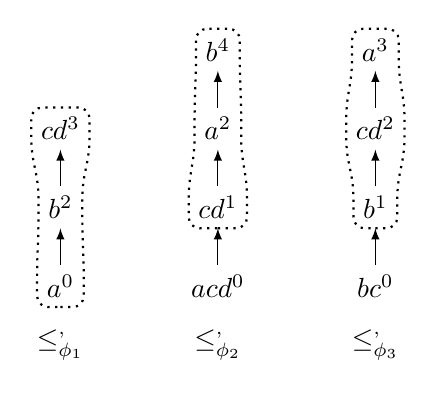
\begin{tikzpicture}
			\node at (0,-0.75){$\le^{\hamming,\:\agg}_{\phi_{1}}$};
			\node at (0,0)(a){$a^{0}$};
			\node at (0,1)(b){$b^{2}$};
			\node at (0,2)(cd){$cd^{3}$};
			\path[-latex](a)edge(b)(b)edge(cd);
			\draw[thick,dotted,rounded corners=4]
				(a.south)--
				(a.south east)--
				(a.north east)--
				(b.south east)--
				(b.north east)--
				(cd.south east)--
				(cd.north east)--
				(cd.north)--
				(cd.north west)--
				(cd.south west)--
				(b.north west)--
				(b.south west)--
				(a.north west)--
				(a.south west)--
				(a.south);

			\node at (2,-0.75){$\le^{\hamming,\:\agg}_{\phi_{2}}$};
			\node at (2,0)(acd){$acd^{0}$};
			\node at (2,1)(cd){$cd^{1}$};
			\node at (2,2)(a){$a^{2}$};
			\node at (2,3)(b){$b^{4}$};
			\path[-latex](acd)edge(cd)(cd)edge(a)(a)edge(b);
			\draw[thick,dotted,rounded corners=4]
				(cd.south)--
				(cd.south east)--
				(cd.north east)--
				(a.south east)--
				(a.north east)--
				(b.south east)--
				(b.north east)--
				(b.north)--
				(b.north west)--
				(b.south west)--
				(a.north west)--
				(a.south west)--
				(cd.north west)--
				(cd.south west)--
				(cd.south);

			\node at (4,-0.75){$\le^{\hamming,\:\agg}_{\phi_{3}}$};
			\node at (4,0)(bc){$bc^{0}$};
			\node at (4,1)(b){$b^{1}$};
			\node at (4,2)(cd){$cd^{2}$};
			\node at (4,3)(a){$a^{3}$};
			\path[-latex](bc)edge(b)(b)edge(cd)(cd)edge(a);
			\draw[thick,dotted,rounded corners=4]
				(b.south)--
				(b.south east)--
				(b.north east)--
				(cd.south east)--
				(cd.north east)--
				(a.south east)--
				(a.north east)--
				(a.north)--
				(a.north west)--
				(a.south west)--
				(cd.north west)--
				(cd.south west)--
				(b.north west)--
				(b.south west)--
				(b.south);
		\end{tikzpicture}			
	\end{minipage}
	\caption{
		Preorders generated using Hamming distances
		and an aggregation function $\agg$
		for the profile $\P=(\phi_i)_{1\le i \le 3}$.
		A majority cycle between $a$, $b$ and $cd$
		means that there is no weak Condorcet winner 
		with respect to $\P$ and $\mu$,
		for $[\mu]=\{a,b,cd\}$.
		The fact that none of the models of $\mu$ is 
		in the top choices of more than two agents in 
		$\P$ means that there is no majority-supported 
		outcome	with respect to $\P$ and $\mu$ outcome either.
	}
	\label{fig:5-condorcet-majr-empty}
\end{figure}

\begin{xmpl}{Weak Condorcet winners do not always exist}{5-condorcet-majr-empty}
	For the set of atoms $\Atoms=\{a,b,c,d\}$,
	consider a profile $\P=(\phi_i)_{1\le i \le 3}$,
	with $[\phi_{1}]=\{a\}$, $[\phi_{2}]=\{acd\}$ and $[\phi_{3}]=\{bc\}$,
	and a constraint $\mu$,
	with $[\mu]=\{a,b,cd\}$.
	The Hamming distances from each of the formulas in $\P$ to 
	each of the models of $\mu$, 
	together with the preorders $\le^{\hamming,\:\agg}_{\phi_{i}}$
	on the models of $\mu$,	for $i\in\{1,2,3\}$,
	are depicted in Figure \ref{fig:5-condorcet-majr-empty}.

	Note that there is no weak Condorcet winner with respect to $\P$ and $\mu$. 
	For instance, the support of $a$ over $b$ is $\supp^{\hamming,\:\agg}_{\mu}(a,b)=\{1,2\}$,
	while the support of $b$ over $a$ is $\supp^{\hamming,\:\agg}_{\mu}(b,a)=\{3\}$,
	which means that $a$ beats $b$ in a head to head election.
	However, $\supp^{\hamming,\:\agg}_{\mu}(a,cd)=\{1\}$ and $\supp^{\hamming,\:\agg}_{\mu}(cd,a)=\{2,3\}$,
	which means that $a$ loses to $cd$ in a head to head contest.
	The same holds for all other pairs of models of $\mu$.
	Likewise, there is no majority-supported outcome
	with respect to $\P$ and $\mu$,
	since none of the models of $\mu$ is in the top choices of more 
	than two of the agents in $\P$.
\end{xmpl}

Example \ref{ex:5-condorcet-majr-empty} shows that 
the postulates just introduced are best understood
by looking at what they expect of the preorders describing the profile.
To make this connection more precise, we present a set of 
properties meant to apply to an $\L^n$-assignment $\as$ on interpretations
that represents an $\L^{n}$-merging operator.
To make sense of the following properties, 
recall from Section \ref{sec:2-choice-functions} that a weak Condorcet winner
with respect to a preference profile and a set of alternatives is an alternative that
gets at least as much support as every other alternative in the set.
The following properties are meant to apply for any 
set $N=\{1,\dots, n\}$ of agents, $\L$-profile $\P=(\phi_i)_{1\le i \le n}$,
interpretations $w_1$ and $w_2$
and sets of interpretations $\W$, $\W_1$, $\W_2$:

\begin{description}
	\item[($\oom{\NOND}$)] There is no agent $i$ such that $\le_{\P}=\le_{\phi_i}$,
		for any profile $\P=(\phi_i)_{1\le i \le n}$.	
	\item[($\oom{\WPRT}$)] If $w_{1}\le_{\phi_i}w_2$, for all $i\in N$, then $w_1 \le_{\P} w_2$.
	\item[($\oom{\SPRT}$)] If $w_{1}\le_{\phi_i}w_2$, for all $i\in N$, 
	and there exists $j\in N$ such that $w_1<_{\phi_j}w_2$, then $w_1 <_{\P} w_2$.
	\item[($\oom{\CSOV}$)] There exists a profile $\P$ such that $w_1\le_{\P}w_2$,
	for any $w_1\in\W_1$ and $w_2\in\W_2$.
	\item[($\oom{\COND}$)] If $w$ is a weak Condorcet winner with respect to $(\le_{\phi_i})_{1\le i\le n}$ and $\W$, 
		then $w\le_\P w'$, for any $w'\in\W$.
	\item[($\oom{\MAJR}$)] If $w_1\le_{\phi_i}w_2$ for a majority of $i\in N$,
		then $w_1\le_{\P}w_2$.
\end{description}

An $\L$-assignment $\as$ on interpretations 
is \emph{non-dictatorial}, \emph{weak} and \emph{strong} Pareto efficient, 
\emph{Condorcet consistent} and \emph{majority consistent} if it satisfies 
properties $\oom{\NOND}$, $\oom{\WPRT}$, $\oom{\SPRT}$, $\oom{\COND}$ and $\oom{\MAJR}$,
respectively.
The properties just introduced map neatly onto the postulates presented earlier.
Since these postulates were tailored specifically to capture solution concepts
from voting theory, this comes as no surprise.

\begin{thm}{}{5-repr-evenhandedness}
	If $\me$ is an $\L^{n}$-merging operator that satisfies postulates $\ppm{0-1}$ and $\ppm{3}$
	and $\as$ is a total $\L^n$-assignment on interpretations that represents it,
	then the following equivalences hold:
	\begin{description}
		\item[(1)] $\me$ satisfies postulate $\ppm{\NOND}$ if and only if $\as$ satisfies property $\oom{\NOND}$.
		\item[(2)] $\me$ satisfies postulate $\ppm{\WPRT}$ if and only if $\as$ satisfies property $\oom{\WPRT}$.
		\item[(3)] $\me$ satisfies postulate $\ppm{\SPRT}$ if and only if $\as$ satisfies property $\oom{\SPRT}$.
		\item[(4)] $\me$ satisfies postulate $\ppm{\CSOV}$ if and only if $\as$ satisfies property $\oom{\CSOV}$.
		\item[(5)] $\me$ satisfies postulate $\ppm{\COND}$ if and only if $\as$ satisfies property $\oom{\COND}$.
		\item[(6)] $\me$ satisfies postulate $\ppm{\MAJR}$ if and only if $\as$ satisfies property $\oom{\MAJR}$.
	\end{description}
\end{thm}
\begin{prf*}{}{}%
	For a comment on the role of postulates $\ppm{0-1}$ and $\ppm{3}$, 
	see the comment at the beginning of the proof for Theorem \ref{thm:5-repr-insensitivity-syntax}.

	For Equivalence (1), we have that the existence of an agent $i$ 
	such that $\me_{\mu}(\P)=\me_{\mu}(\phi_{i})$,
	for any profile $\P=(\phi_i)_{1\le i \le n}$ and constraint $\mu$,
	is equivalent to the fact that 
	$w_1 \le_{\P}w_2$ if and only if $w_1 \le_{\phi_{i}}w_2$, for any interpretations $w_1$ and $w_2$,
	i.e., to the fact that $\le_{\P} = \le_{\phi_{i}}$.

	For Equivalence (2), suppose first that $\me$ satisfies postulate $\ppm{\WPRT}$ 
	and assume that $\as$ does not satisfy property $\oom{\WPRT}$.
	This means that there exist interpretations $w_1$ and $w_2$
	such that $w_1 \le_{\phi_{i}}$, for $i\in N$, and $w_2 \le_{\P}w_1$. 
	Taking the constraint $\px_{1,2}$ yields a contradiction with postulate $\ppm{\WPRT}$.
	Conversely, suppose $\as$ satisfies property $\oom{\WPRT}$ and $\me$ does not satisfy
	postulate $\ppm{\WPRT}$. This implies that there exists 
	$w_1\in[\me_{\mu}(\phi_{1})\land\dots\land \me_{\mu}(\phi_{n})]$
	such that $w_1\notin[\me_{\mu}(\P)]$.
	The latter conclusion implies,
	by postulates $\ppm{0}$ and $\ppm{1}$ and the assumption that 
	$\le_{\P}$ is total,
	that there exists an interpretation $w_2\in[\me_{\mu}(\P)]$
	such that $w_2 <_{\P}w_1$. 
	The former conclusion, however, implies that $w_1 \le_{\phi_{i}} w_2$, 
	for any $i\in N$,
	which, together with property $\oom{\WPRT}$, implies that $w_1 \le_{\P} w_2$.
	We have thus arrived at a contradiction.

	For Equivalence (3), suppose first that $\me$ satisfies postulate $\ppm{\SPRT}$ 
	and assume that $\as$ does not satisfy property $\oom{\SPRT}$.
	This means that there exist interpretations $w_1$ and $w_2$
	such that $w_1 \le_{\phi_{i}} w_2$, for $i\in N$, $w_1 <_{j}w_2$,
	for some $j\in N$ and, furthermore, that $w_2 \le_{\P} w_1$.
	This means that 
	$\me_{\px_{1,2}}(\phi_{1})\land\dots\land \me_{\px_{1,2}}(\phi_{n})$
	is consistent, which, by postulate $\ppm{\SPRT}$, implies that 
	$w_2\in[\me_{\px_{1,2}}(\phi_{j})]$.
	But this is a contradiction. 
	Conversely, suppose $\as$ satisfies property $\oom{\SPRT}$ and $\me$ does not satisfy
	postulate $\ppm{\SPRT}$. This implies that there exists an interpretation 
	$w_1\in[\me_{\mu}(\P)]$ such that $w_1\notin[\me_{\mu}(\phi_{1})\land\dots\land \me_{\mu}(\phi_{n})]$.
	The latter conclusion,
	together with postulates $\ppm{0}$, $\ppm{1}$ and the assumption that $\as$ is total,
	implies that there exists $j\in N$ such that 
	$w_1\notin[\me_{\mu}(\phi_{j})]$.
	The assumption that $\me_{\mu}(\phi_{1})\land\dots\land \me_{\mu}(\phi_{n})$
	is consistent implies that there exists $w_2\in[\me_{\mu}(\phi_{1})\land\dots\land \me_{\mu}(\phi_{n})]$.
	Putting the last two facts together implies that 
	$w_2\le_{\phi_i}w_1$, for every $i\in N$, and $w_2<_{\phi_{j}}w_1$,
	which, by property $\oom{\SPRT}$, yields that $w_2<_{\P}w_1$.
	But this contradicts the fact that $w_1\in[\me_{\mu}(\P)]$.

	For Equivalence (4), the statement is trivially true if $\mu_1\land\mu_2$ is inconsistent,
	hence we only look at the case when $\mu_1\land\mu_2$ is consistent.
	For one direction, suppose $\me$ satisfies postulate $\ppm{\CSOV}$:
	then, for any sets $\W_1$ and $\W_2$ of interpretations, take 
	the $\L$-proxies of $\W_1\cup\W_2$ and $\W_1$,
	i.e., two propositional formulas $\px_{\W_1\cup\W_2}$ and $\px_{\W_1}$ such that 
	$[\px_{\W_1\cup\W_2}]=\W_1\cup\W_2$ and $[\px_{\W_1}]=\W_1$.
	Using postulate $\ppm{\CSOV}$, we have that there exists a profile $\P$ 
	such that $\me_{\px_{\W_1\cup\W_2}}(\P)\land\px_{\W_1}\equiv \px_{\W_1\cup\W_2}\land\px_{\W_1}$,
	which implies that $[\me_{\px_{\W_1\cup\W_2}}(\P)]=\W_1$.
	This, in turn, implies that $\min_{\le_{\P}}[\px_{\W_1\cup\W_2}]=\W_1$,
	from which the conclusion follows.
	Conversely, we take $\W_1=[\mu_1\land\mu_2]$ and $\W_2=[\mu_1]$.

	For Equivalence (5), we remark that $w_1 \le^{\me}_{\P}w_2$
	is equivalent to $w_1\in[\me_{\px_{1,2}}(\P)]$, 
	which is equivalent to the fact that $w_1\in\min_{\le_{\P}}[\px_{1,2}]$,
	or $w_1{\le_{\P}}w_2$,
	for any total preorder $\le_{\P}$ used to represent $\me$.
	This implies that an interpretation $w^{\ast}$ being a weak Condorcet winner
	with respect to $(\le_{\phi_i})_{1\le i \le n}$ and $\mu$ is equivalent 
	to $w^{\ast}$ being a weak Condorcet winner with respect to the preference
	profile $\PP=(\le_{\phi_{i}})_{1\le i \le n}$ and $[\mu]$.
	If $\me$ is an $\L^{n}$-merging operator that satisfies postulate $\ppm{\COND}$,
	then a weak Condorcet winner $w^{\ast}$ with respect to $\PP$ and a set of interpretations 
	$\W$ will be a model of $\me_{\px_{\W}}(\P)$, and this implies that 
	$w^{\ast}\in\min_{\le_{\P}}[\px_{\W}]$,
	i.e., that $w^{\ast} \le_{\P} w$, for any interpretation $w\in[\W]$.
	Conversely, a weak Condorcet winner $w^{\ast}$ with respect to $\P$ and $\mu$
	is a weak Condorcet winner with respect to 
	$(\le_{\phi_i})_{1\le i \le n}$ and $[\mu]$ and, by property $\oom{\COND}$, it holds that 
	$w^{\ast}\le_{\P}w$, for any $w\in[\mu]$,
	which implies that $w^{\ast}\in\min_{\le_{\P}}[\mu]$,
	or $w^{\ast}\in[\me_{\mu}(\P)]$.

	For Equivalence (6) we use the same observation as above to argue that 
	$w^{\ast}$ being a majority-supported outcome with respect to $\P$ and $\mu$
	is equivalent to $w^{\ast}$ being a majority-supported outcome with respect 
	to $(\le_{\phi_i})_{1\le i \le n}$ and $[\mu]$, which then yields the conclusion.
\end{prf*}

Theorem \ref{thm:5-repr-evenhandedness} makes it clear what an $\L$-assignment $\as$ on interpretations
needs to look like if a merging operator $\me$ represented by it 
is to satisfy the postulates introduced in this section.
The immediate next question, however, is whether existing distance-based 
merging operators actually manage to select majority-supported outcomes, when they exist,
or weak Condorcet winner, when they exist, or whether they are non-dictatorial or resolvable.
For some of these properties there exists a useful shortcut,
since it turns out that they follow directly from postulate $\ppm{0-8}$.

\begin{prp}{}{5-nond-csov-prt}
	If $\me$ is an $\L^{n}$-merging operator that satisfies postulates $\ppm{0-8}$,
	then $\me$ also satisfies postulates $\ppm{\NOND}$, $\ppm{\CSOV}$, $\ppm{\WPRT}$ and $\ppm{\SPRT}$.
\end{prp}
\begin{prf*}{}{}%
	For postulate $\ppm{\NOND}$,
	suppose agent 1, with beliefs $\phi_1$, is a dictator for the merging operator $\me$. 
	Choose a formula $\phi_2$ such that $\phi_1 \land \phi_2$ is inconsistent 
	and a constraint $\mu = \phi_1 \lor \phi_2$.
	Since agent 1 is a dictator, we have that $\me_{\mu}(\phi_1, \phi_2)\equiv \me_{\mu}(\phi_1)$.
	Since $\mu \land \phi_1 $ is consistent, by postulate $\ppm{2}$ 
	it follows that $\me_{\mu}(\phi_1) \equiv \phi_1\land \mu \equiv \phi_1$. 
	At the same time we have that $\me_\mu(\phi_1,\phi_2) \land \phi_1$ is consistent, 
	and thus, by postulate $\ppm{4}$, 
	it holds that $\me_{\mu}(\phi_1,\phi_2) \land \phi_2$ is consistent as well. 
	We then have a contradiction with the fact that $\phi_1 \land \phi_2$ is inconsistent.

	For postulate $\ppm{\CSOV}$,
	if $\mu_1\land\mu_2$ is inconsistent, the conclusion is immediate.
	If $\mu_1\land\mu_2$ is consistent,
	take a profile $\P = (\phi)$,
	where $\phi=\mu_1\land\mu_2$.
	Clearly, $\phi \land \mu_1$ is consistent, hence by postulate $\ppm{2}$ 
	it follows that $\me_{\mu}(\P) \equiv \phi\land\mu_1\equiv\mu_1\land\mu_2$.

	Postulates $\ppm{\WPRT}$ and $\ppm{\SPRT}$ follow directly from postulates $\ppm{5}$ and $\ppm{6}$.
\end{prf*}

In the case of postulate $\ppm{\MAJR}$, the situation turns out to be different:
the presence of postulate $\ppm{2}$ actually precludes any merging operator 
from satisfying $\ppm{\MAJR}$.

\begin{prp}{}{5-majr}
	If $\me$ is an $\L^{n}$-merging operator that satisfies postulate $\ppm{2}$, 
	then $\me$ does not satisfy postulate $\ppm{\MAJR}$.
\end{prp}
\begin{prf*}{}{}%
	Take a profile $\P=(\phi_i)_{1\le i \le 3}$,
	with $[\phi_{1}]=[\phi_2]=\{\emptyset,a\}$
	and $[\phi_{3}]=\{\emptyset\}$, 
	and a constraint $\mu$ with $[\mu]=\{\emptyset,a\}$.
	Postulate $\ppm{2}$ implies that 
	$[\me_{\mu}(\P)]=[\phi_1\land\phi_2\land\phi_3\land\mu]=\{\emptyset\}$.
	Thus, even though $a$ is a top choice of two out of the three agents,
	$a$ does not make the list of winning interpretations.
\end{prf*}

The idea behind Proposition \ref{prop:5-majr} is that, under postulate $\ppm{2}$,
any agent has veto power over an interpretation $w$: by not including $w$ 
in its top choices, i.e., by not making $w$ a model of its submitted opinion, 
the agent makes sure that $w$ is not part of the result:
and this will happen even if $w$ is supported by a majority of the agents. 
Incidentally, postulate $\ppm{2}$ precludes the possibility that anything along the lines
of a \emph{plurality-supported outcome} will be guaranteed to be in the result. 

We now have all the pieces of information we need to 
determine where the main distance-based operators 
stand in relation to the postulates introduced in this section.

\begin{table}\centering
	\begin{tabular}{ccccccc}
		\toprule
						 & $[\phi_{1-3}]$ & $[\phi_{4-5}]$ & $[\phi_{6}]$ & $[\phi_{7}]$ &&\\
		$\dd_{\hamming}$ & $3\cdot\{a\}$     & $2\cdot\{bc\}$ & $\{b\}$ & $\{acd\}$ & $\dd_{\hamming}^{\ssum}(\P,\bullet)$ & $\dd_{\hamming}^{\leximax}(\P,\bullet)$\\
																 \midrule
			$a$          &     $3\cdot 0$     &   $2\cdot 3$        & $2$ & $2$ & $10$ & $(3,3,2,2,0,0,0)$   \\
			$b$          &     $3\cdot 1$     &   $2\cdot 1$        & $0$ & $4$ & $\mathbf{9}$  & $(4,1,1,1,1,1,0)$   \\
			$cd$          &    $3\cdot 2$     &   $2\cdot 2$        & $3$ & $1$ & $14$ & $\mathbf{(3,2,2,2,2,2,1)}$   \\
			\bottomrule
	\end{tabular}	
	\caption{
		Outcome $a$ is the only weak Condorcet winner 
		with respect to	the profile $\P=(\phi_i)_{1\le i \le 7}$ 
		and $\mu$, where $[\mu]=\{a,b,cd\}$,
		but $a$ is selected by neither $\me^{\hamming,\:\ssum}$
		nor by $\me^{\hamming,\:\leximax}$.
	}
	\label{tab:5-hsum-hlmax-not-condorcet}
\end{table}

\begin{prp}{}{5-dist-ops-evenhandedness}
	If $\agg$ is either the $\ssum$, $\leximax$ or $\leximin$
	aggregation function, then the following statements hold:
	\begin{description}
		\item[(1)] postulates $\ppm{\NOND}$, $\ppm{\WPRT}$, $\ppr{\SPRT}$ and $\ppm{\CSOV}$
		are satisfied by all operators $\me^{\hamming,\:\agg}$ and $\me^{\drastic,\:\agg}$;
		\item[(2)] postulate $\ppm{\COND}$ is satisfied by operators $\me^{\drastic,\:\agg}$,
			but by neither of the operators $\me^{\hamming,\:\agg}$;
		\item[(3)] postulate $\ppm{\MAJR}$ is satisfied by neither of the operators $\me^{\drastic,\:\agg}$
			and $\me^{\hamming,\:\agg}$.
	\end{description}
\end{prp}
\begin{prf*}{}{}%
	Since the operators $\me^{\hamming,\:\agg}$ 
	and $\me^{\drastic,\:\agg}$, 
	for $\agg\in\{\ssum,\leximax,\leximin\}$, 
	satisfy postulates $\ppm{0-8}$, then,
	by Proposition \ref{prop:5-nond-csov-prt}, they 
	also satisfy postulates $\ppm{\NOND}$, $\ppm{\WPRT}$, $\ppr{\SPRT}$, $\ppm{\CSOV}$,
	and by Proposition \ref{prop:5-majr} they do not satisfy 
	postulate $\ppm{\MAJR}$.
	This shows that Statements (1) and (3) hold.

	For Statement (2) and operators $\me^{\drastic,\:\agg}$ recall first that 
	all three operators considered here are equivalent,
	so proving the claim for $\me^{\drastic,\:\ssum}$ will suffice. 
	Note, as well, that $\dd_{\drastic}^{\ssum}(\P,w)$ essentially 
	counts the number of agents in $N$,
	who have $w$ as their model, for any interpretation $w$,
	and $\me^{\drastic,\:\ssum}$ selects the interpretations in $[\mu]$
	that occur most often as models of agents in $N$.
	We have, then, that if $w^{\ast}$ is a weak Condorcet winner with respect 
	to $\phi$ and $\mu$, then $\supp^{\drastic,\:\ssum}_{\mu}(w^{\ast},w)\ge\supp^{\drastic,\:\ssum}(w,w^{\ast})$,
	for any interpretation $w\in[\mu]$.
	This means that $w^{\ast}$ occurs as a model of $\phi_{i}$ for at least as many 
	agents $i\in N$ than any other interpretation $w\in[\mu]$,
	which, as per the previous observation, implies that $w^{\ast}\in[\me^{\drastic,\:\ssum}_{\mu}(\P)]$.	 

	For Statement (2) and operators $\me^{\hamming,\:\ssum}$ and $\me^{\hamming,\:\leximax}$, 
	take the profile $\P=(\phi_i)_{1\le i \le 7}$,
	with $[\phi_{1}]=[\phi_{2}]=[\phi_{3}]=\{a\}$,
	$[\phi_{4}]=[\phi_{5}]=\{bc\}$,
	$[\phi_{6}]=\{b\}$,
	$[\phi_{7}]=\{acd\}$,
	and a constraint $\mu$ such that 
	$[\mu]=\{a,b,cd\}$.
	The Hamming distances from $\phi_{i}$, for $1\le i\le 7$,
	to every model of $\mu$,
	together with the aggregated distances for 
	the $\ssum$ and $\leximax$ aggregation function, 
	are depicted in Table \ref{tab:5-hsum-hlmax-not-condorcet}.

	Note that $a$ is the only weak Condorcet winner with respect to 
	$\P$ and $\mu$, since the size of its support over $b$ and $cd$
	is $4$ in both cases. 
	In other words, $[\COND_{\mu}(\P)]=\{a\}$.
	However, $a$ is selected by neither $\me^{\hamming,\:\ssum}$
	nor $\me^{\hamming,\:\leximax}$, since $[\me^{\hamming,\:\ssum}_{\mu}(\P)]=\{b\}$
	and $[\me^{\hamming,\:\leximax}_{\mu}(\P)]=\{cd\}$.

	For Statement (2) and operator $\me^{\hamming,\:\leximin}$,
	a simpler counterexample will suffice. 
	Take the profile $\P=(\phi_i)_{1\le i \le 3}$,
	with $[\phi_{1}]=[\phi_{2}]=\{\emptyset\}$ and $[\phi_{3}]=\{ab\}$,
	and a constraint $\mu$ with $[\mu]=\{a,ab\}$.
	We have that 
	$\dd_{\hamming}^{\leximin}(\P,a)=(1,1,1)$
	and
	$\dd_{\hamming}^{\leximin}(\P,ab)=(0,2,2)$,
	which means that $[\me^{\hamming,\:\leximin}_{\mu}(\P)]=\{ab\}$.
	However, $a$ is the only weak Condorcet winner 
	(and even the majority supported outcome)
	with respect to $\P$ and $\mu$.
\end{prf*}
























\section{Responsiveness}\label{sec:5-responsiveness}
This section proposes an assortment of properties 
meant to ensure that changes in the profile 
produce an intuitive, and expected, change of the outcome,
i.e., that the merging operation is responsive to 
the structure of the profile.
Since these properties involve expanding the set $N=\{1,\dots,n\}$ 
of agents in the profile
%  and the set $\Atoms$ of atoms, 
we need to make sure that there is a stock of agents 
% and atoms 
on hand if needed to supplement the profile 
% and $\Atoms$ 
with new elements.
We assume, therefore, that the set of agents $N$
who supply formulas to the merging operator 
% and $\Atoms$ are 
is part of some larger subsets,
whose elements can be invoked upon request.
% Adding atoms to $\Atoms$ is akin to the idea  adding a candidate to an election.
That being said, we can introduce the following postulates,
intended to hold for any profile
$\P=(\phi_i)_{1\le i \le n}$, 
and constraints $\mu$, $\mu_1$, $\mu_2$:
% and atoms $p$ and $q$:

\begin{description}
	\item[($\ppm{\MONO}$)] $\me_{\mu}(\P + \phi_{n+1}) \land \me_{\mu}(\phi'_{n+1})\models\me_{\mu}(\P+\phi'_{n+1})$.
 
	\item[($\ppm{\PART}$)] If $\me_\mu(\P) \land \phi_{n+1}$ is consistent, 
		then $\me_\mu(\P) \land \phi_{n+1} \models \me_{\mu}(\P+\phi_{n+1})$. 

	\item[($\ppm{\RSYM}$)] If $\me_\mu(\P)$ is complete and $\mu$ has more than one model, 
		then $\me_\mu(\phi_1,\dots,\phi_n) \nvDash\me_{\mu}(\lnot\phi_1,\dots,\lnot\phi_n)$.

	\item[($\ppm{\RSVB}$)] If $\me_{\mu_1}(\P)\land\mu_2$ is consistent, 
		there is $\phi_{n+1}$ such that $\me_{\mu_1}(\P+\phi_{n+1})\equiv \me_{\mu_1}(\P)\land \mu_2$.

	% \item[($\ppm{\INDC}$)] If $p\in\Atoms$ and $q\notin\Atoms$, 
	% 	then $\me_\mu(\phi_1,\dots,\phi_n) \equiv \me_{\mu}(\phi_1\land(p\leftrightarrow q),\dots,\phi_n\land(p\leftrightarrow q))$. 

	% \item[($\ppm{\CONS}$)] $\me_{\mu}(\P_1) \land \dots \land \me_{\mu}(\P_n) \models \me_\mu(\P_1+\dots+\P_n)$.

	% \item[($\ppm{\HOMG}$)] $\me_\mu(\P) \equiv \me_{\mu}(\P+\dots+\P)$.

	% \item[($\ppm{\SLFA}$)] $\me_{\mu}(\P +\me_\mu(\P)) \equiv \me_\mu(\P)$.
\end{description}

Postulate $\ppm{\MONO}$, where `$\MONO$' stands for \emph{monotonicity},
says that if $\phi_{n+1}$ agrees with the profile $\P+\phi_{n+1}$ 
to a certain extent when the constraint is $\mu$,
then this agreement is carried over when merging the formulas in the profile $\P+\phi'_{n+1}$.
Intuitively, the profile $\P+\phi'_{n+1}$ can be thought of as being obtained from 
the profile $\P+\phi_{n+1}$ by replacing $\phi_{n+1}$ with $\phi'_{n+1}$:
it is as if agent $n+1$ considers its options, 
changes its mind and submits $\phi'_{n+1}$ instead of $\phi_{n+1}$.
Postulate $\ppm{\MONO}$ then says that if this change of mind
(i.e., after submitting $\phi'_{n+1}$)
is in line with the 
result obtained previously
(i.e., when submitting $\phi_{n+1}$), then the originally agreed upon result 
should not be changed. 
In other words, if the agent maintains its support 
for a raft of issues that were already included 
in the final result, then these issues are still endorsed
by the merging process
when the agent submits a formula that expresses as much, if not more, 
support for these issues.
In this, postulate $\ppm{\MONO}$ attempts to recreate the monotonicity property 
found in voting theory:
a voting system is monotone if the winning alternative in an election cannot be 
turned into a non-winner by one voter moving this alternative up in its ranking, 
while keeping the rest of the ranking fixed.
The intuition behind our formalization stems from seeing the models of 
$\me_\mu(\P)$ as the winners in the election where the models of $\mu$ 
are candidates and the formulas in $\P$ are the voters,
and will come out more clearly when modeled 
as a property for assignments on interpretations,
to come shortly.
% Thus, if any candidates elected by the profile $\P_1+ \P_2$ are also elected by the profile $\P_3$ alone, 
% then monotonicity would require that the same  candidates should also be elected when we replace $\P_2$ with $\P_3$ in $\P_1 + \P_2$.
% The idea, to put it succinctly, is that a winner stays a winner, if its position is only increased in the votes. 
Note that postulate $\ppm{\MONO}$ as put forward here is slightly 
different from the way it was originally presented \cite{HaretPW16}.
The change is made in order to bring the postulate closer to the monotonicity
property as featured in social choice. Though arguable whether the present formulation
achieves this completely, it is certainly an interesting property to consider.

Postulate $\ppm{\PART}$, where `$\PART$' stands for \emph{participation},
refers to a phenomenon that in voting is linked to the \textit{no-show paradox}.
A voting rule is vulnerable to this type of paradox
if it is possible to change the winner from candidate $c_i$ to candidate $c_j$ 
by adding a vote in which candidate $c_i$ is strictly preferred to candidate $c_j$.
In a merging scenario, we prevent this by adding a formula $\phi$ to a given profile $\P$ and
requiring that $\me_{\mu}(\P+\phi)$ should not be `worse' than $\me_\mu(\P)$ with respect to $\phi$.

Postulate $\ppm{\RSYM}$, where `$\RSYM$' stands for \emph{reversal symmetry},
harkens back to an eponymous property in voting.
A voting rule satisfies reversal symmetry if the 
winner (assumed to be unique) of an election does not stay a winner
if all votes are reversed.
In a merging scenario, we interpret the condition of having a unique winner 
as the outcome of merging 
being a complete formula (i.e., a formula with exactly one model), 
and we take reversing the vote to mean that every formula 
is replaced with its negation.
% Notice that we require the outcome to be a complete formula to reflect the requirement 
% of a unique winner in the voting setting.

Postulate $\ppm{\RSVB}$, where `$\RSVB$' stands for \emph{resolvability},
says that the output of merging can be refined up to an arbitrary degree 
by adding just one formula to $\P$.
In a voting scenario resolvability 
requires that any winner can be made 
the unique winner by adding a single vote \cite{Tideman06},
and postulate $\ppm{\RSVB}$ models this intuition. 


% Postulate $\ppm{\INDC}$ concerns \emph{independence of clones}.
% In voting theory two candidates are clones if they are ranked next to each other, and in the same pattern, in all votes.
% A voting system is independent of clones if a non-winning candidate cannot be made a winner by adding clones to the election. 
% In a merging scenario we think of a clone as a fresh variable $q$ that mirrors an existing variable $p$,
% in the sense that agents uniformly consider them as equivalent, i.e., can adopt $p\leftrightarrow q$ as part of the belief. 
% Postulate $\ppm{\INDC}$ requires that the merging result does not change when adding a clone to a profile. 

% Postulate $\ppm{\CONS}$ concerns \emph{consistency},
% which in a voting scenario requires that if an election is arbitrarily divided into sub-elections 
% and there is a candidate $c$ that is a winner in all of the them, then $c$ is also a winner in the original election.
% In a merging scenario, we formalize this by splitting the merging task across different profiles 
% ($\P_1$, \dots, $\P_n$), which can be thought of as parts of a larger profile ($\P_1+\dots+\P_n$). 
% Postulate $\ppm{\CONS}$ then requires that any outcomes universally accepted across the subprofiles
% are also accepted in the profile obtained by concatenating them.

% Postulate $\ppm{\HOMG}$ concerns \emph{homogeneity},
% which in a voting system requires that the result cannot be changed by duplicating each vote a number of times. 
% In a merging scenario this translates as postulate $\ppm{\HOMG}$, 
% saying that the outcome of merging does not change if the profile is expanded by multiple copies of itself. 

% Postulate $\ppm{\SLFA}$ concerns \emph{self agreement},
% and requires that the merging outcome stays the same if $\P$ is added back to the profile and the merging 
% process is run again.

With the postulates in place, we want to switch now to the semantic
view, and see how the postulates are represented at the level off
an $\L$-assignment $\as$ on interpretations.
Thus, given such an assignment, 
consider the following properties,
expected to hold for any $\L$-profile $\P=(\phi_i)_{1\le i \le n}$,
propositional formulas $\phi_{n+1}$, $\phi'_{n+1}$,
sets $\W_1$ and $\W_2$ of interpretations
and interpretations $w_1$ and $w_2$:

\begin{description}
	\item[($\oom{\MONO}$)] If $w_1\le_{\P_1+\phi_{n+1}}w_2$ and $w_1\le_{\phi'_{n+1}}w_2$, then $w_1\le_{\P+\phi'_{n+1}}w_2$.
	\item[($\oom{\PART}$)] If $w_1 \le_{\P}w_2$ and $w_1\in[\phi_{n+1}]$, then $w_1 \le_{\P+\phi_{n+1}}w_2$. 
	\item[($\oom{\RSYM}$)] If $w_1 <_{(\phi_i)_{1\le i \le n}}w_2$, then $w_2<_{(\lnot\phi_i)_{1\le i \le n}}w_1$. 
	\item[($\oom{\RSVB}$)] If $w_1 \le_{\P}w_2$, for every interpretation $w_1\in\W_1$ and $w_2\in\W_2$,
		then there exists a formula $\phi_{n+1}$ such that $w_1<_{\P+\phi_{n+1}}w_2$, 
		for every interpretation $w_1\in\W_1$ and $w_2\in\W_2$.
\end{description}

\begin{thm}{}{5-repr-responsiveness}
	If $\me$ is an $\L^{n}$-merging operator satisfying postulates $\ppm{0-1}$ and $\ppm{3}$,
	and $\as$ is a total $\L^n$-assignment on interpretations that represents it,
	then the following equivalences hold:
	\begin{description}
		\item[(1)] $\me$ satisfies postulate $\ppm{\MONO}$ if and only if $\as$ satisfies property $\oom{\MONO}$.
		\item[(2)] $\me$ satisfies postulate $\ppm{\PART}$ if and only if $\as$ satisfies property $\oom{\PART}$.
		\item[(3)] $\me$ satisfies postulate $\ppm{\RSYM}$ if and only if $\as$ satisfies property $\oom{\RSYM}$.
		\item[(4)] $\me$ satisfies postulate $\ppm{\RSVB}$ if and only if $\as$ satisfies property $\oom{\RSVB}$.
	\end{description}
\end{thm}
\begin{prf*}{}{}%
	For Equivalence (1), suppose first that $\me$ satisfies postulate $\ppm{\MONO}$
	and take interpretations $w_1$ and $w_2$ such that 
	$w_1 \le_{\P+\phi_{n+1}}w_2$ and $w_1 \le_{\phi'_{n+1}}w_2$.
	This implies that $w_1\in\min_{\le_{\P+\phi_{n+1}}}[\px_{1,2}]$ and $w_1\in\min_{\le_{\phi'_{n+1}}}[\px_{1,2}]$,
	i.e., that $w_1\in[\me_{\px_{1,2}}(\P+\phi_{n+1})\land \me_{\px_{1,2}}(\phi'_{n+1})]$.
	Using postulate $\ppm{\MONO}$, we conclude that $w_1\in[\me_{\px_{1,2}}(\P+\phi'_{n+1})]$.
	From this it follows that $w_1\le_{\P+\phi'_{n+1}}w_2$.
	Conversely, suppose $\as$ satisfies property $\oom{\MONO}$ and 
	$\me_{\mu}(\P+\phi_{n+1})\land \me_{\mu}(\phi'_{n+1})$ is consistent.
	The latter fact implies that there exists an interpretation 
	$w_1\in[\me_{\mu}(\P+\phi_{n+1})\land \me_{\mu}(\phi'_{n+1})]$.
	Taking an arbitrary interpretation $w_2\in[\mu]$ and applying property $\oom{\MONO}$, 
	we conclude that 
	$w_1 \le_{\P+\phi'_{n+1}}w_2$, which implies that $w_1\in[\me_{\mu}(\P+\phi'_{n+1})]$.

	For Equivalence (2), suppose $\me$ satisfies postulate $\ppm{\PART}$
	and take two interpretations $w_1$ and $w_2$ such that $w_1 \le_{\P} w_2$.
	We then obtain that $w_1\in[\me_{\px_{1,2}}(\P)\land\phi_{n+1}]$, 
	which, by postulate $\ppm{\PART}$, implies that $w_1\in[\me_{\px_{1,2}}(\P+\phi_{n+1})]$
	and hence $w_1 \le_{\P+\phi_{n+1}}w_2$.
	Conversely, if $\as$ satisfies property $\oom{\PART}$, 
	then for any $w_1\in[\me_{\mu}(\P)\land\phi_{n+1}]$ and 
	interpretation $w_2\in[\mu]$, it follows that $w_1 \le_{\P+\phi_{n+1}}w_2$,
	which implies the conclusion.

	For Equivalence (3), suppose $\me$ satisfies postulate $\ppm{\RSYM}$
	and take two distinct interpretations $w_1$ and $w_2$ such that $w_1 <_{(\phi_i)_{1\le i \le n}} w_2$.
	This implies that $[\me_{\px_{1,2}}(\phi_1,\dots,\phi_n)]=\{w_1\}$, i.e., that $\me_{\px_{1,2}}(\phi_1,\dots,\phi_n)$
	is complete. Applying postulate $\ppm{\RSYM}$, it follows that $[\me_{\px_{1,2}}(\lnot\phi_1,\dots,\lnot\phi_n)]=\{w_2\}$,
	showing that property $\oom{\RSYM}$ is satisfied.
	Conversely, if $\as$ satisfies property $\oom{\RSYM}$ and $[\me_{\mu}(\phi_1,\dots,\phi_n)]=\{w_1\}$,
	then $w_1<_{(\phi_i)_{1\le i \le n}}w_2$, for any other interpretation $w_2\in[\mu]$, which must exist as
	per the assumption of postulate $\ppm{\RSYM}$. Applying property $\oom{\RSYM}$ results in 
	$w_2<_{(\lnot\phi_i)_{1\le i \le n}}w_1$, which delivers the conclusion.	

	For Equivalence (4), suppose $\me$ satisfies postulate $\ppm{\RSVB}$
	and take sets of interpretations $\W_1$ and $\W_2$
	such that $w_1 \le_{\P}w_2$, for any $w_1\in\W_1$ and $w_2\in\W_2$.
	It follows that $\W_1\subseteq\min_{\le_{\P}}(\W_1\cup\W_2)$
	and hence that $[\me_{\px_{\W_1\cup\W_2}}(\P)\land \px_{\W_1}]=\W_1$.
	Postulate $\ppm{\RSVB}$ implies that there exists a formula 
	$\phi_{n+1}$ such that $\me_{\px_{\W_1\cup\W_2}}(\P+\phi_{n+1})\equiv\me_{\px_{\W_1,\W_2}}(\P)\land\px_{\W_1}$,
	from which it follows that $[\me_{\px_{\W_1\cup\W_2}}(\P+\phi_{n+1})]=\W_1$,
	and hence $w_1<_{\P+\phi_{n+1}}w_2$,
	for any $w_1\in\W_1$ and $w_2\in\W_2$.
	Conversely, suppose $\as$ satisfies property $\oom{\RSYM}$
	and take formulas $\mu_1$ and $\mu_2$ such that $\me_{\mu_1}(\P)\land\mu_2$
	is consistent.
	This implies that $w_1 \le_{\P}w_2$, for every $w_1\in\min_{\le_{\P}}[\mu_1]\cap[\mu_2]$
	and $w_2\in[\mu_1]$ and hence, by property $\oom{\RSVB}$,
	that there exists a formula $\phi_{n+1}$ such that 
	$w_1 <_{\P+\phi_{n+1}}w_2$, for every $w_1\in\min_{\le_{\P}}[\mu_1]\cap[\mu_2]$
	and $w_2\in[\mu_1]$.
	From this it follows that $\me_{\mu_1}(\P+\phi_{n+1})\equiv \me_{\mu_1}(\P)\land \mu_2$
\end{prf*}

\begin{prp}{}{5-part-rsvb}
	If $\me$ is an $\L^{n}$-merging operator that satisfies postulates $\ppm{0}$ and $\ppm{1}$,
	then the following statements hold:
	\begin{description}
		\item[($1$)] if $\me$ satisfies postulates $\ppm{2}$ and $\ppm{5}$, 
			then $\me$ satisfies postulate $\ppm{\PART}$.
		\item[($2$)] if $\me$ satisfies postulates $\ppm{2}$, $\ppm{5}$ and $\ppm{6}$ 
			then $\me$ satisfies postulate $\ppm{\RSVB}$.
	\end{description}
\end{prp}
\begin{prf*}{}{}%
	For Statement (1), take $w\in[\me_{\mu}(\P)\land\phi_{n+1}]$.
	By postulate $\ppm{0}$ it follows that $w\in[\mu]$.
	Since $w\in[\phi_{n+1}\land\mu]$, then by postulate $\ppm{2}$ 
	we can conclude that $w\in[\me_{\mu}(\phi_{n+1})]$
	and thus that $w\in[\me_{\mu}(\P)\land\me_{\mu}(\phi_{n+1})]$.
	Using postulate $\ppm{5}$ it follows that $w\in[\me_{\mu}(\P+\phi_{n+1})]$.

	For Statement (2), take $\phi_{n+1}\equiv \me_{\mu_1}(\P)\land\mu_2$.
	Both postulates $\ppm{0}$ and $\ppm{1}$ we have that 
	$(\me_{\mu_1}(\P)\land\mu_2)\land\mu_1\equiv\me_{\mu_1}(\P)\land\mu_2$,
	Thus, using postulate $\ppm{2}$, we have that 
	$\me_{\mu_1}(\me_{\mu_1}(\P)\land\mu_2)\equiv \me_{\mu_1}(\P)\land\mu_2$.
	This shows, among other things, that
	$\me_{\mu_1}(\P)\land \me_{\mu_1}(\me_{\mu_1}(\P)\land\mu_2)$ is consistent,
	which,
	by postulates $\ppm{5}$ and $\ppm{6}$ implies that
	$\me_{\mu_1}(\P)\land \me_{\mu_1}(\me_{\mu_1}(\P)\land\mu_2)\equiv \me_{\mu_1}(\P+(\me_{\mu_1}(\P)\land\mu_2))$.
	Using the previously derived equivalences,
	we can conclude that 
	$\me_{\mu_1}(\P)\land \me_{\mu_1}(\me_{\mu_1}(\P)\land\mu_2)\equiv \me_{\mu_1}(\P)\land\mu_2$.
\end{prf*}

Before laying down the full picture of how existing merging operators 
fare with respect to the postulates in this section,
a quick observation on the reversal symmetry postulate $\ppm{\RSYM}$
will help make things clearer. Reflection on postulate $\ppm{\RSYM}$,
and even more so on its semantic counterpart, property $\oom{\RSYM}$,
shows that the demands it places on an assignment are considerable:
in particular, property $\oom{\RSYM}$ requires that 
replacing all formulas in an $\L$-profile $\P$ with their negation 
should reverse all strict comparisons in the preorder 
corresponding to the negated profile.
When coupled with the observation that negating the formulas 
in an $\L$-profile may create a profile equivalent to the original one,
this leads to the conclusion that the only feasible 
preorder that can represent such a situation is one 
in which all interpretations are on the same level.

\begin{lem}{}{5-rsym}
	If $\me$ is an $\L^{n}$-merging operator that satisfies 
	postulates $\ppm{0-1}$, $\ppm{3}$ and $\ppm{\RSYM}$, then 
	$\me_{\top}(\phi,\lnot\phi)\equiv\top$,
	for any propositional formula $\phi$.
\end{lem}
\begin{prf*}{}{}%
	We know, by Theorem \ref{thm:3-merging-repr}, that $\me$
	is represented by a total, syntax insensitive and m-faithful 
	$\L^n$-assignment $\as$ on interpretations.
	By Theorem \ref{thm:5-repr-responsiveness},
	we can also conclude that $\as$ satisfies property $\oom{\RSYM}$.
	Suppose, now, that there exists a propositional formula $\phi$
	such that $\me_{\top}(\P)\not\equiv\top$,
	where $\P$ is the $\L$-profile $\P=(\phi,\lnot\phi)$.
	This implies that there exist interpretations $w_1$ and $w_2$
	such that $w_1<_{\P}w_2$.
	By property $\oom{\RSYM}$, we conclude that $w_2<_{\P'}w_1$,
	where $\P'$ is the $\L$-profile $\P'=(\lnot\phi,\lnot(\lnot\phi))$.
	It is easy to see, however, that $\P$ and $\P'$ are equivalent profiles
	and hence, by postulate $\ppm{3}$,
	that $\me_{\mu}(\P)\equiv \me_{\mu}(\P')$,
	for any propositional formula $\mu$.
	But this implies that $\le_{\P}=\le_{\P'}$,
	which contradicts the conclusions derived previously.
\end{prf*}

With all these results in hand, we can now have a full picture
of how the main merging operators stand up 
against the responsiveness properties 
put forward in this section.

\begin{table}\centering
	\begin{tabular}{cccccc}
		\toprule
		 & $\P=(\phi_1)$ & $(\phi_2)$ &&&\\
		 & $\{\emptyset,a\}$ & $\{abc\}$ & $\dd_{\hamming}^{\ssum}(\P+\phi_2,\bullet)$ & $\dd_{\hamming}^{\leximax}(\P+\phi_2,\bullet)$ & $\dd_{\hamming}^{\leximin}(\P+\phi_2,\bullet)$\\\midrule
		$\emptyset$ & $0$ & $3$ & $3$ & $(3,0)$ & $(0,3)$\\
		$abc$       & $2$ & $0$ & $\mathbf{2}$ & $\mathbf{(2,0)}$ & $\mathbf{(0,2)}$\\
		\bottomrule
	\end{tabular}
	\caption{
		Hamming distances from $\P=(\phi_1)$ and $\phi_2$ to each model of $\mu$,
		with $[\phi_{1}]=\{\emptyset,a\}$, $[\phi_2]=\{abc\}$ and $[\mu]=\{\emptyset,abc\}$,
		together with the aggregated distances using the $\ssum$, $\leximax$ and $\leximin$
		aggregation functions.
	}
	\label{tab:5-mono-1}
	vspace{1.5em}

	\begin{tabular}{cccccc}
		\toprule
		 & $\P=(\phi_1)$ & $(\phi'_2)$ &&&\\
		 & $\{\emptyset,a\}$ & $\{ab\}$ & $\dd_{\hamming}^{\ssum}(\P+\phi'_2,\bullet)$ & $\dd_{\hamming}^{\leximax}(\P+\phi'_2,\bullet)$ & $\dd_{\hamming}^{\leximin}(\P+\phi'_2,\bullet)$\\\midrule
		$\emptyset$ & $0$ & $2$ & $\mathbf{2}$ & $\mathbf{(2,0)}$ & $\mathbf{(0,2)}$\\
		$abc$       & $2$ & $1$ & $3$ & $(2,1)$ & $(1,2)$\\
		\bottomrule
	\end{tabular}
	\caption{
		Hamming distances from $\P=(\phi_1)$ and $\phi_2$ to each model of $\mu$,
		with $[\phi_{1}]=\{\emptyset,a\}$ as above, 
		$[\phi_2]=\{abc\}$ and $[\mu]=\{\emptyset,abc\}$,
		together with the aggregated distances using the $\ssum$, $\leximax$ and $\leximin$
		aggregation functions.
	}
	\label{tab:5-mono-2}
\end{table}

\begin{table}\centering
	\begin{tabular}{cccccc}
		\toprule
														 & 
		$\P$ 											 &  
		$\phi_{n+1}$ 									 & 
		$\phi'_{n+1}$ 									 & 
		$\dd_{\drastic}^{\ssum}(\P+\phi_{n+1},\bullet)$  & 
		$\dd_{\drastic}^{\ssum}(\P+\phi'_{n+1},\bullet)$ \\
				 										 \midrule
		$w_1$   & $k+1$ & $0$ & $0$ & $k+1$ & $k+1$\\
		$w_2$   & $k$   & $1$ & $0$ & $k+1$ & $k$\\
		\bottomrule
	\end{tabular}
	\caption{
		Drastic distances from $\P$, $\phi_{n+1}$ and $\phi'_{n+1}$ to $w_1$ and $w_2$,
		together with the aggregated distances using the $\ssum$ aggregation functions,
		for a stereotypical case that does not satisfy property $\oom{\MONO}$:
		outcome $w_1$ is winning after adding $\phi_{n+1}$ to $\P$,
		but it loses out to $w_2$ when agent $n+1$ submits a formula 
		that weakens the support for $w_1$.
	}
	\label{tab:5-mono-3}
\end{table}

\begin{prp}{}{5-dist-ops-responsiveness}
	If $\agg$ is either the $\ssum$, $\leximax$ or $\leximin$ aggregation function,
	then the following statements hold:
	\begin{description}
		\item [($1$)] merging operators $\me^{\hamming,\:\agg}$	and $\me^{\drastic,\:\agg}$
			all satisfy postulates $\ppm{\PART}$ and $\ppm{\RSVB}$;
		\item[($2$)] merging operators $\me^{\hamming,\:\agg}$ do not satisfy postulate $\ppm{\RSYM}$,
			but operators $\me^{\drastic,\:\agg}$ satisfy it;
		\item[($3$)] neither of the merging operators $\me^{\hamming,\:\agg}$ and $\me^{\drastic,\:\agg}$
			satisfies postulate $\ppm{\MONO}$;
		% \item[($4$)] neither of the merging operators $\me^{\hamming,\:\agg}$ and $\me^{\drastic,\:\agg}$
		% 	satisfies postulate $\ppm{\INDC}$.
	\end{description}
\end{prp}
\begin{prf*}{}{}%
	Statement (1) follows from Corollary \ref{cor:3-merging-d-agg-induced-operator},
	showing that all the operators considered here satisfy postulate $\ppm{0-8}$
	and Proposition \ref{prop:5-part-rsvb}, showing that these postulates guarantee 
	satisfaction of postulates $\ppm{\PART}$ and $\ppm{\RSVB}$.

	For Statement (2) and operators $\me^{\hamming,\:\agg}$,
	take the set of atoms $\Atoms=\{a,b\}$ and a profile $\P=(\phi_1,\phi_2)$,
	with $[\phi_{1}]=\{\emptyset,b,ab\}$ and $[\phi_{2}]=\{a\}$.
	Notice that $\me^{\hamming,\:\agg}_{\top}(\P)\not\equiv\top$,
	for all of the aggregation functions considered and thus,
	by Lemma \ref{lem:5-rsym}, the merging operators do not 
	satisfy postulate $\ppm{\RSYM}$.

	For Statement (2) and operators $\me^{\drastic,\:\agg}$,
	recall that operators $\me^{\drastic,\:\agg}$ are equivalent,
	for all aggregation functions considered here,
	and that the aggregated distance $\dd^{\agg}(\P,w)$ from an $\L$-profile $\P$
	to an interpretation $w$ essentially keeps track of the number of 
	formulas in $\P$ that have $w$ as their model;
	obviously, if we replace the formulas in $\P$ with their negation, then this number 
	is reversed. More precisely, if $\P'$ is the profile obtained by 
	replacing every formula in $\P$ with its negation, then 
	$\dd_{\drastic}^{\agg}(\P',w)=n-\dd_{\drastic}^{\agg}(\P,w)$, 
	where $n$ is the number of agents 
	in the profile. This implies that if $w_1<^{\drastic,\:\agg}_{\P}w_2$,
	then $w_2<^{\drastic,\:\agg}_{\P'}w_1$,
	for any interpretations $w_1$ and $w_2$,
	which shows that $\as^{\drastic,\:\agg}$ satisfies property $\oom{\RSYM}$
	and, by Theorem \ref{thm:5-repr-responsiveness},
	postulate $\ppm{\RSYM}$ as well.

	For Statement (3) and the operators $\me^{\hamming,\:\agg}$, 
	take the alphabet $\Atoms=\{a,b,c\}$,
	the $\L$-profile $\P=(\phi_1)$,
	with $[\phi_{1}]=\{\emptyset,a\}$, 
	the propositional formulas $\phi_{2}$ and $\phi'_{2}$
	with $[\phi_2]=\{abc\}$ and $[\phi'_2]=\{ab\}$,
	and a constraint $\mu$ with $[\mu]=\{\emptyset,abc\}$.
	The Hamming distances from $\P+\phi_2$ and $\P+\phi'_2$
	to each model of $\mu$, 
	together with the aggregated distances according to the 
	$\ssum$, $\leximax$ and $\leximin$ aggregation functions 
	are shown in Tables \ref{tab:5-mono-1} and \ref{tab:5-mono-2},
	respectively.
	We have that $[\me^{\hamming,\:\agg}_{\mu}(\P+\phi_2)]=\{abc\}$,
	for all of the aggregation functions considered here,
	and thus $abc<^{\hamming,\:\agg}_{P+\phi_2}\emptyset$.
	At the same time, we also have that 
	$abc<^{\hamming,\:\agg}_{\phi'_{2}}\emptyset$,
	but $\emptyset<^{\hamming,\:\agg}_{\P+\phi'_{2}}abc$.

	For Statement (3) and the operators $\me^{\drastic,\:\agg}$,
	recall first that operators defined using the aggregation 
	functions considered here are all equivalent,
	so we make the argument only for $\me^{\drastic,\:\ssum}$.
	Take, now, the alphabet $\Atoms=\{a,b\}$,
	the $\L$-profile $\P=(\phi_1)$,
	with $[\phi_{1}]=\{a\}$, 
	the propositional formulas $\phi_{2}$ and $\phi'_{2}$
	with $[\phi_2]=\{\emptyset\}$ and $[\phi'_2]=\{\emptyset,a\}$,
	and a constraint $\mu$ with $[\mu]=\{\emptyset,a\}$.
	We obtain that $\emptyset\approx^{\drastic,\:\ssum}_{\P+\phi_2} a$,
	$\emptyset\approx^{\drastic,\:\ssum}_{\phi'_2} a$
	but $a<^{\drastic,\:\ssum}_{\P+\phi'_2} \emptyset$,
	which constitutes a counterexample to property $\oom{\MONO}$:
	an edge case, to be sure, but a counterexample nonetheless,
	the general form of which is depicted in Table \ref{tab:5-mono-3}.
\end{prf*}
















\section{Strategyproofness}\label{sec:5-strategyproofness}
In this section we look at issues related to the manipulability 
and strategyproofness of merging procedures.
Issues of strategic reasoning cannot be avoided
if, as we have argued, merging is to be used as a 
framework for collective decision making.
A significant concern in any deliberation scenario is that the agents 
involved may have an incentive to misrepresent their positions, 
and thus manipulate the aggregation result, 
if doing so can bring them an advantage.
Hence, an understanding of the potential 
for manipulation of any aggregation procedure is a 
prerequisite to its successful 
deployment in any real world context.
That merging operators are apt to be manipulated 
is illustrated by a quick example.

\begin{table}\centering
\begin{tabular}{cccccccc}
	\toprule
					  &
	$[\phi_1]$        &
	$[\truth{\phi}_2]$        &
	$[\manip{\phi}_2]$        &
	$[\phi_3]$        &
	$[\phi_4]$        &
					  &
					  \\

	$\dd_\hamming$    & 
	$\{ab,abc\}$      & 
	$\{ab, ac, abc\}$ &
	$\{a\}$           & 
	$\{b\}$           & 
	$\{c\}$           &  
	$\dd_{\hamming}^{\ssum}(\truth{\P},\bullet)$ & 
	$\dd_{\hamming}^{\ssum}(\manip{\P},\bullet)$ \\\midrule

	$ab$              &
	$0$               &
	$0$               & 
	$1$               & 
	$1$               & 
	$3$       & 
	$4$       & 
	$5$               \\

	$ac$              &
	$1$               &
	$0$               & 
	$1$               & 
	$3$               & 
	$1$       & 
	$5$       & 
	$6$               \\

	$bc$              &
	$1$               &
	$1$               & 
	$3$               & 
	$1$               & 
	$1$       & 
	$4$       & 
	$6$               \\
	\bottomrule
	\end{tabular}
	\caption{
		Academy member $2$, whose truthful
		position is expressed by $\truth{\phi}_{2}$,
		can obtain a better result by submitting 
		$\manip{\phi}_{2}$.
	}
	\label{tab:5-manip-motivation}
\end{table}

\begin{xmpl}{}{5-manip-motivation}
	Recall the example of the four Academy members
	who have to agree on two nominees for the 
	\emph{Best Director} category, 
	out of three possible directors:
	Alma Har'el ($a$), Bong Joon Ho ($b$) and C\'eline Sciamma ($c$).
	The opinions of the Academy members are 
	$\phi_1 = a\land b$,
	$\phi_2 = a\land (b\lor c)$,
	$\phi_3 = \lnot a\land b \land \lnot c$.
	and
	$\phi_4 = \lnot a \land\lnot b\land c$,
	and the constraint is 
	$\mu=(a\land b\land \lnot c)\lor(a\land\lnot b\land c)\lor(\lnot a\land b\land c)$.
	Suppose, now, that merging is done with the operator $\me^{\hamming,\:\ssum}$.
	We saw in Example \ref{ex:3-merging-distance-ops}
	that $[\me^{\hamming,\:\ssum}_\mu(\P)]=\{ab,bc\}$,
	for $\P=(\phi_1,\phi_2,\phi_3,\phi_4)$,
	i.e., the result is to nominate either Alma Har'el and Bong Joon Ho,
	or Bong Joon Ho and C\'eline Sciamma.
	The existence of two possible lineups indicates that the result suggested 
	by the operator $\me^{\hamming,\:\ssum}$ is not decisive,
	but is something like a tie between two equally acceptable outcomes.
	Note, however, that both outcomes agree on $b$, such that 
	$b$ seems like a safe bet for whatever the final result turns out to be.

	Switching our focus to Academy member $2$, whose preferences are 
	given by $\phi_2 = a\land (b\lor c)$, we see that they also vacillate 
	between a few options, i.e., $ab$, $ac$, $abc$,
	but throughout all of them $a$ occurs consistently. 
	We may assume, therefore, that Academy member $2$ would prefer 
	an outcome that guarantees that $a$ will be part of it to
	an outcome that does not.

	Suppose, now, that Academy member $2$ decides to act strategically
	and, instead of submitting their true position,
	which we will henceforth denote by $\truth{\phi}_{2}=\phi_{2}$,
	submits the formula $\manip{\phi}_{2}=a\land\lnot b\land\lnot c$.
	If we write $\manip{\P}$ for the profile $\manip{\P}=(\phi_{1},\manip{\phi}_{2},\phi_3,\phi_4)$,
	then we obtain that $[\me^{\hamming,\:\ssum}_{\mu}(\manip{\P})]=\{ab\}$,
	with the details of this computation spelled out in Table \ref{tab:5-manip-motivation}.
	This is an outcome that is certainly more appealing to Academy member $2$,
	since it contains the atom $a$, which figures among all of 
	Academy member $2$'s most preferred outcomes.
\end{xmpl}

In Example \ref{ex:5-manip-motivation} we see that one of the 
agents in the profile has an incentive to misrepresent its 
true position, since by doing so it can pull the merging result
closer to its true opinion.
Our purpose in this section will be to formalize the reasoning 
involved in this type of strategic thinking:
we will need a way to quantify what it means for a given result to count 
as better for an agent than a different result,
and analyze the extent to which the primary merging operators 
are vulnerable to manipulation.

\subsubsection{Acceptance notions}
As we see in Example \ref{ex:5-manip-motivation},
merging operators may output multiple interpretations,
all of which can be seen as winning outcomes.
In decision terms, this translates as inconclusiveness with respect to the final verdict.
Thus, the set of winning outcomes produced by a merging operator 
is not always expected to be the final step in a reasoning process: 
without further means, such a set of interpretations 
does not give a direct answer to which atoms, i.e., issues,
are to be ultimately accepted.
One can view the winning set as a ``tie'' 
between all the interpretations in the set. 
If the decision procedure needs to be explicit about every issue under consideration, 
then a further reasoning mechanism is required, amounting to a method of breaking ties.
To this end, we employ well established acceptance notions 
from the field of knowledge representation and reasoning: 
skeptical and credulous consequences \cite{StrasserA19}.

An \emph{acceptance function $\acc$} is a function 
$\acc\colon\L\rightarrow 2^{\Atoms}$
that maps propositional formulas to sets of atoms in $\P$.
We say that \emph{$\acc(\phi)$ are the accepted atoms of $\phi$}.
For a formula $\phi$, we define the following acceptance notions:
\begin{align*}
\skept(\phi) = \bigcap_{w \in [\phi]}w, && \cred(\phi) = \bigcup_{w\in [\phi]}w.
\end{align*}

For a formula $\phi$, 
an atom is \emph{skeptically accepted} if it is in $\skept(\phi)$,
i.e., if it is true in all models of $\phi$,
and \emph{credulously accepted} 
if it is in $\cred(\phi)$, i.e., if it is true in at least one model of $\phi$.
We will follow established convention in writing the skeptical and credulously accepted
atoms as words with the atoms as letters.
% \footnote{We note that the notions of \emph{skeptical} (cautious) and \emph{credulous} (brave) consequences are not uniformly used throughout the literature. 
% 	For instance, skeptical consequences may be defined as those consequences that follow (e.g., by classical  logic) from all formulas in a set of formulas, and skeptical acceptance may refer to membership of an object in all sets of a given set of sets. We make use of the latter interpretation.}
Skeptical acceptance is equivalent to atom-wise logical entailment, 
and credulous acceptance indicates support of an atom in at least one model. 

\begin{xmpl}{Acceptance notions}{5-acceptance-notions}
	In Example \ref{ex:5-manip-motivation}, we obtain that 
	$[\me^{\hamming,\:\ssum}_{\mu}(\truth{\P})]=\{ab,bc\}$.
	Thus, it holds that 
	$\skept(\me^{\hamming,\:\ssum}_{\mu}(\truth{\P}))=b$ 
	and $\cred(\me^{\hamming,\:\ssum}_{\mu}(\truth{\P}))=abc$. 
\end{xmpl}

The acceptance notions introduced here focus on positive literals.
Thus, we say that $p\in\skept(\phi)$ if the atom $p$ is in every model of $\phi$,
but we do not treat acceptance of negative literals in a similar fashion,
i.e., we are not explicit about atoms that are in none of the models of a formula,
and that can thus be thought of as uniformly rejected.
This asymmetry is not unusual in a social choice context,
where rejection of a candidate is often assimilated to non-acceptance, 
but would be worth looking at 
in a more extensive treatment of acceptance notions. 

It turns out that there is a duality relation between the 
indices and aggregation operators defined via skeptical and credulous acceptance
that we will want to exploit.
Recall that the \emph{dual $\dual{\phi}$ of a formula $\phi$} is obtained
by replacing every literal in $\phi$ with its negation.
If $\P=(\phi_i)_{1\le i \le n}$ is an $\L$-profile, 
then \emph{the dual $\dual{\P}$ of $\P$} is the profile 
defined as $\dual{\P}=(\dual{\phi}_i)_{1\le i \le n}$.
If $w$ is an interpretation, 
\emph{the dual $\dual{w}$ of $w$} is the complement of $w$.
If $\W$ is a set of interpretations, 
\emph{the dual $\dual{\W}$ of $\W$} is the set of interpretations defined as
$\dual{\W}=\set{\dual{w}\mid w\in\W}$.
For a propositional formula $\phi$ we have that 
$\dual{[\phi]}=\mods{\dual{\phi}}$. 
% Interestingly, a duality also holds with respect to merging operators
% and the acceptance notions.

\begin{prp}{}{5-duals-accepted-atoms}
	If $\P$ is a propositional profile, 
	$\mu$ is a constraint, 
	$\dd\in\set{\dd_\hamming, \dd_\drastic}$ is a distance function, 
	and $\agg\in\set{\ssum,\leximax,\leximin}$ is an aggregation function,
	then it holds that 
	$\dual{\skept(\me_\mu^{\dd,\:\agg}(\P))}\equiv\cred(\me^{\dd,\:\agg}_{\dual{\mu}}(\dual{\P}))$.
\end{prp}
\begin{prf*}{}{}%
	It is straightforward to see that $\dd(w_1,w_2) = \dd(\dual{w_1},\dual{w_2})$,
	for any two interpretations $w_1$ and $w_2$ and 
	distance function $\dd\in\{\dd_{\drastic},\dd_{\hamming}\}$.
	Using this, we can conclude that 
	$\dual{\me^{\dd,\:\agg}_{\mu}(\P)}\equiv \me^{\dd,\:\agg}_{\dual{\mu}}(\dual{\P})$.
	Next, we have that for an atom $p$, 
	it holds that $p\notin\skept(\me^{\dd,\:\agg}_{\mu}(\P))$ if and only if 
	there exists an interpretation $w\in\mods{\me^{\dd,\:\agg}_{\mu}(\P)}$ such that $p\notin w$.
	Using the previous observation,
	this is equivalent to $p\in\dual{w}$, for some interpretation 
	$\dual{w}\in[\me^{\dd,\:\agg}_{\dual{\mu}}(\dual{\P})]$,
	which is in turn equivalent to $p\in\cred(\me^{\dd,\:\agg}_{\dual{\mu}}(\dual{\P}))$.
\end{prf*}

Proposition~\ref{prop:5-duals-accepted-atoms} builds on an interesting symmetry 
exhibited by the merging operators we work with:
the result of merging a profile $\P$ under a constraint $\mu$ 
and the result of merging $\dual{\P}$ under constraint $\dual{\mu}$ turn out
to be themselves duals of each other. This allows us, once we have found some 
instance related to the skeptical index,
to automatically adapt it to the credulous index. 

\begin{xmpl}{Merging and duals}{5-duals-main-notions}
	For the set of atoms $\Atoms=\set{a,b}$, 
	take a profile $\P=(\phi_1,\phi_2)$, with
	$\phi_1 = {a\rightarrow b}$, $\phi_2=\lnot a$ and $\mu= a$.
	We obtain $\mods{\me_\mu^{\hamming,\:\ssum}(\P)}=\{ab\}$, 
	and $\skept(\me_\mu^{\hamming,\:\ssum}(\P))=ab$.
	Taking the duals, we have $\dual{\phi_1}=\lnot a\rightarrow\lnot b$,
	$\dual{\phi_2}=a$ and $\dual{\mu}=\lnot a$.
	Notice that $\mods{\phi_1}=\set{\emptyset,b,ab}$
	and $\mods{\dual{\phi_1}}=\set{ab,a,\emptyset}=\set{\dual{\emptyset},\dual{b},\dual{ab}}=\dual{\mods{\phi_1}}$,
	i.e., the models of the dual of $\phi_1$ are the duals of the models of $\phi_1$.
	We obtain that $[\me^{\hamming,\:\ssum}_{\dual{\mu}}(\dual{\P})]=\set{\emptyset}$,
	which is the same as $\mods{\dual{\me_\mu^{\hamming,\:\ssum}(\P)}}$ (this equality also holds more generally).
	Lastly, $\dual{\skept(\me_\mu^{\hamming,\:\ssum}(\P))}=\cred(\me^{\hamming,\:\ssum}_{\dual{\mu}}{\dual(\P)})$.
\end{xmpl}

Manipulation occurs when an agent, called \emph{the strategic agent},
can influence the merging result in its favor by submitting a formula different from its truthful one. 
In the following we will typically represent the agent's truthful position by a formula $\truth{\phi}$, 
and the formula with which it manipulates as $\manip{\phi}$.
We represent the strategic agent's contribution by appending 
its reported formula to a pre-existing profile $\P$,
with $\truth{\P}=\P+\truth{\phi}$  
and $\manip{\P} = \P+\manip{\phi}$ 
being the truthful and manipulated profiles, respectively.
Intuitively, this is as if the strategic agent joins the aggregation process 
\emph{after} everyone else has submitted their positions.
This is merely a notational choice, meant to improve readability, and no generality is lost in this way: 
since all operators we will look at in this section satisfy the anonymity postulate $\ppm{\ANON}$,
as presented in Section \ref{sec:5-syntax},
the result never depends on the order of the formulas in the profile. 



\subsubsection{Constructive and destructive manipulation with respect to an atom}
One of the most basic forms of manipulation is one in which
the strategic agent has a specific atom $p$ that it targets for acceptance: 
the strategic agent may want to see $p$ obtain accepted (or rejected) in the final result.
This sets up the stage for the notions we will introduce now
and which we call,
along the lines of similar concepts from the field of social choice \cite{ConitzerW2016},
\emph{constructive} and \emph{destructive} manipulation.
A profile $\P$, 
constraint $\mu$,
distance $\dd$, 
aggregation function $\agg$ and acceptance notion $\acc$
are assumed in most definitions,
but, in the interest of concision,
are explicitly referred to only under pain of ambiguity.
Unless otherwise stated, $\dd$ ranges over $\{\dd_\drastic,\dd_\hamming\}$ 
and $\agg$ over $\{\ssum,\leximax\}$.

The strategic agent \emph{constructively $\acc$-manipulates $\P$ with respect to $p$ using $\manip{\phi}$} 
if $p\notin\acc(\me_\mu(\P+\truth{\phi}))$ and $p\in\acc(\me_\mu(\P+\manip{\phi}))$,
and \emph{destructively $\acc$-manipulates $\P$ with respect to $p$ using $\manip{\phi}$} 
if $p\in\acc(\me_\mu(\P+\truth{\phi}))$ and $p\notin\acc(\me_\mu(\P+\manip{\phi}))$.
Intuitively, an agent constructively $\acc$-manipulates with respect to $p$ if it can make
$p$ be in the accepted atoms of the aggregation result by submitting $\manip{\phi}$ instead of $\truth{\phi}$;
similarly, an agent destructively manipulates with respect to $p$ 
if it can kick $p$ out of the accepted atoms of the result.
We say that an operator $\me$ is \emph{$\acc$-strategyproof}
if there is no profile $\P$, constraint $\mu$, atom $p$ and formulas $\truth{\phi}$ and $\manip{\phi}$ s.t.\  
the strategic agent, having $\truth{\phi}$ as its truthful position,
$\acc$-manipulates $\P$, either constructively or destructively,
with respect to $p$ using $\manip{\phi}$. 

We first note that,
if $\truth{\phi}$ is the strategic agent's truthful position,
any instance of constructive manipulation with respect to $p$ using $\manip{\phi}$
is also an instance of destructive manipulation with respect to $p$, obtained by swapping
$\truth{\phi}$ and $\manip{\phi}$ as the truthful and manipulating formulas, respectively.
Next, our results regarding duality 
(see Proposition \ref{prop:5-duals-accepted-atoms}) imply the following duality for manipulation. 

\begin{prp}{}{5-manipulation-con-des-acceptance-duality}
	A strategic agent constructively (or destructively) 
	$\skept$-manipulates $\P$ with respect to $p$ if and only if
	it destructively (or, respectively, constructively) $\cred$-manipulates $\dual{\P}$ 
	with respect to $p$ using $\dual{\manip{\phi}}$, 
	with $\dual{\truth{\phi}}$ as its truthful position and $\dual{\mu}$ as the constraint.
\end{prp}
\begin{prf*}{}{}%
	Assume an instance of constructive $\skept$-manipulation with respect to $p$.
	If $p\notin\skept(\me^{\dd,\:\agg}_{\mu}(\P+\truth{\phi}))$, 
	then $p\in\dual{\skept(\me^{\dd,\:\agg}_{\mu}(\P+\truth{\phi}))}$.
	Thus, by Proposition~\ref{prop:5-duals-accepted-atoms},
	it holds that $p\in\cred(\me^{\dd,\:\agg}_{\dual{\mu}}(\dual{P}+\dual{\truth{\phi}}))$.
	Similarly, we get that if $p\in\skept(\me^{\dd,\:\agg}_{\dual{\mu}}({\P+\manip{\phi}}))$,
	then $p\notin\cred(\me^{\dd,\:\agg}_{\dual{\mu}}(\dual{P}+\dual{\manip{\phi}}))$.
	We have obtained, in this way, an instance of destructive $\cred$-manipulation with respect to $p$.
	
	The proof going from an instance of destructive $\skept$-manipulation to an instance of 
	constructive $\skept$-manipulation with respect to $p$ is entirely analogous.
\end{prf*}

In other words, an instance of constructive $\skept$-manipulation 
has a direct counterpart, via the duals,
in an instance of destructive $\cred$-manipulation, 
and likewise for destructive $\skept$-manipulation and constructive $\cred$-manipulation.
This simplifies our study as we can focus on only one acceptance notion, with results for 
the other notion following by Proposition~\ref{prop:5-manipulation-con-des-acceptance-duality}.

\begin{xmpl}{Constructive $\skept$-manipulation to destructive $\cred$-manipulation}{5-constructive-skept-translates-into-destructive-cred}
	In Example \ref{ex:5-manip-motivation}, Academy member $2$
	constructively $\skept$-manipulates the profile $\P=(\phi_1,\phi_3,\phi_4)$
	with respect to the atom $a$, 
	relative to the operator $\me^{\hamming,\:\ssum}$ and constraint 
	$\mu=(a\land b\land \lnot c)\lor (a\land\lnot b\land c)\lor(\lnot a\land b\land c)$, 
	in that $a\notin\skept(\me^{\hamming,\:\ssum}_{\mu}(\truth{\P}))$ 
	but $a\in\skept(\me^{\hamming,\:\ssum}_{\mu}(\manip{\P}))$.
	Consider, now, a merging scenario where every formula is replaced by its dual.
	In this setting, the truthful position of Academy member $2$ 
	is $\dual{\truth{\phi}_2}$:
	we obtain that $[\dual{\truth{\phi}_2}]=\{b,c,bc\}$,
	the constraint is $\dual{\mu}$,
	with $[\dual{\mu}]=\{a,b,c\}$, 
	and the profile is $\dual{\P}$.
	We obtain that $[\me^{\hamming,\:\ssum}_{\dual{\mu}}{\dual(\truth{\P})}]=\{a,c\}$,
	and $a\in\cred(\me^{\hamming,\:\ssum}_{\dual{\mu}}{\dual(\truth{\P})})$.
	However, if Academy member $2$ now submits $\dual{\manip{\phi}_2}$, we obtain that 
	$[\me^{\hamming,\:\ssum}_{\dual{\mu}}(\dual{\P}+\dual{\manip{\phi}_2})]=\{c\}$, 
	with $a\notin\cred(\me^{\hamming,\:\ssum}_{\dual{\mu}}(\dual{\P}+\dual{\manip{\phi}_2}))$.
	Hence, if Academy member $2$'s truthful position is $\dual{\truth{\phi}_2}$,
	then it destructively $\cred$-manipulates $\dual{\P}$ with respect to $a$ using $\dual{\manip{\phi}_2}$.	
\end{xmpl}

Examples \ref{ex:5-manip-motivation} and
\ref{ex:5-constructive-skept-translates-into-destructive-cred} 
already show that the merging operator 
$\me^{\hamming,\:\ssum}$ is constructively $\skept$-manipulable 
(and destructively $\cred$-manipulable).
Indeed, Theorem \ref{thm:5-constructive-destructive-atom-manipulation}
shows that this extends to all operators introduced so far.
Recall that a formula is complete if it has exactly one model.

\begin{thm}{}{5-constructive-destructive-atom-manipulation}
	For any $n\in\mathbb{N}$
	and atom $p\in\Atoms$,
	there exists a profile 
	$\P=(\phi_i)_{1\le i \le n}$ and formulas $\truth{\phi}$, $\manip{\phi}$ 
	such that the strategic agent 
	constructively (and destructively, respectively) 
	$\acc$-manipulates $\P$ with respect to $p$ using $\manip{\phi}$,
	even if $\mu=\top$ and all $\phi_i$, for $i\in\{1,\dots,n\}$, 
	as well as $\truth{\phi}$ and $\manip{\phi}$, are complete.
	The instances of manipulation occur relative to all 
	operators $\me^{\dd,\:\agg}$, for 
	$\dd\in\{\dd_{\drastic},\dd_{\hamming}\}$
	and $\agg\in\set{\ssum,\leximax,\leximin}$.
\end{thm}
\begin{prf*}{}{}%
	Without loss of generality, we can assume the target atom $p$ is $a$.
	We only showcase the constructive $\skept$-manipulation instances, 
	as corresponding $\cred$-manipulation instances can be 
	obtained using Proposition~\ref{prop:5-manipulation-con-des-acceptance-duality}
	and a destructive manipulation instance can be obtained from a constructive manipulation instance
	by swapping $\truth{\phi}$ and $\manip{\phi}$ 
	as the truthful and manipulating base, respectively, of the strategic agent.
	We assume, throughout, that $\mu=\top$.
	
	The following argument applies to operators 
	$\me^{\dd,\:\agg}$, for $\dd\in\{\dd_{\drastic},\dd_{\hamming}\}$
	and $\agg\in\set{\ssum,\leximax,\leximin}$.
	To obtain constructive $\skept$-manipulation, 
	we take $\truth{\phi}=\bigwedge_{p\in\P}\lnot p$. 
	Thus, $[\truth{\phi}]=\{\emptyset\}$
	and $\skept(\truth{\phi})=\emptyset$. 
	We then do a case analysis depending on whether $n$ is odd or even.
	In both cases, the agent manipulates using
	$\manip{\phi}=a\land\bigwedge_{p\in\P,p\neq a}\lnot p$, with $[\manip{\phi}]=\{a\}$.
	Each operator is analyzed in turn.
	
	\emph{Case 1}.
	If $n$ is even, we write $n=2k$, for $k\in\mathbb{N}$.
	For the operators $\me^{\dd,\:\agg}$, 
	for $\dd\in\set{\dd_{\drastic},\dd_{\hamming}}$ and $\agg\in\set{\ssum,\leximax,\leximin}$ 
	we take the profile $\P=(\phi_1,\dots,\phi_{2k})$ 
	such that $\mods{\phi_1}=\dots=\mods{\phi_k}=\set{\emptyset}$ and 
	$\mods{\phi_{k+1}}=\dots=\mods{\phi_{2k}}=\set{a}$. 
	Notice that all bases are complete.
	
	For the operator $\me^{\hamming,\:\ssum}$,
	note that in the truthful profile $\truth{\P}=\P+\truth{\phi}$ we have 
	$\dd_{\hamming}^\ssum(\truth{\P},\emptyset)=k$ and 
	$\dd_{\hamming}^\ssum(\truth{\P},a)=k+1$,
	while for any other interpretation $w$ we get that 
	$\dd_{\hamming}^\ssum(\truth{\P},w)=(\sum_{i=1}^{2k}\delta_i)+\truth{\delta}$,
	where $\delta_i=\dd_{\hamming}^\ssum(\phi_i,w)$ 
	and $\truth{\delta}=\dd_{\hamming}^\ssum(\truth{\phi},w)$.
	It is straightforward to see that $\delta_i\geq 1$, 
	for any $i\in\set{1,\dots,2k}$ and that $\truth{\delta}\geq 1$ as well.
	Thus, $\emptyset <^{\hamming,\:\ssum}_{\P+\truth{\phi}} a$ 
	and $\emptyset <^{\hamming,\:\ssum}_{\P+\truth{\phi}} w$ for any other interpretation $w$,
	i.e., $[\me^{\hamming,\:\ssum}_{\top}(\truth{\P})]=\{\emptyset\}$.
	In the manipulated profile $\manip{\P}=\P+\manip{\phi}$ we get that
	$\dd_{\hamming}^\ssum(\P+\manip{\phi},\emptyset)=k+1$ 
	and $\dd_{\hamming}^\ssum(\P+\manip{\phi},a)=k$,
	while for any other interpretation $w$ we get that 
	$\dd_{\hamming}^\ssum(\truth{\P},w)=(\sum_{i=1}^{2k}\delta_i)+\manip{\delta}$,
	where $\manip{\delta}=\dd_{\hamming}^\ssum(\manip{\phi},w)$.
	It is straightforward to see that $\manip{\delta}\geq 1$ and
	thus $a <^{\hamming,\:\ssum}_{\manip{\P}} \emptyset$ and 
	$a <^{\hamming,\:\ssum}_{\manip{\P}} w$ for any other interpretation $w$,
	i.e., $[\me^{\hamming,\:\ssum}_{\top}(\manip{\P})]=\{a\}$.
	Since $a\notin\skept(\me^{\hamming,\:\ssum}_{\top}(\truth{\P}))$ 
	but $a\in\skept(\me^{\hamming,\:\ssum}_{\top}(\manip{\P}))$, 
	this counts as an instance of constructive manipulation.

	For the operator $\me^{\hamming,\:\leximax}$ 
	we reason analogously as for $\me^{\hamming,\:\ssum}$, 
	and using the same profile $\P$.
	Notice that the following equality holds:
	$$
		\dd_{\hamming}^\leximax(\truth{\P},\emptyset)=(~\underbrace{1,\dots,1}_{k~\text{times}}~,\underbrace{0,\dots,0}_{(k+1)~\text{times}}),
	$$ 
	and:
	$$
		\dd_{\hamming}^\leximax(\truth{\P},a)=(\underbrace{1,\dots,1}_{(k+1)~\text{times}},~\underbrace{0,\dots,0}_{k~\text{times}}~),
	$$
	while:
	$$
		\dd_{\hamming}^\leximax(\truth{\P},w)=\leximax(\delta_1,\dots,\delta_{2k},\truth{\delta}),
	$$ 
	for any other interpretation $w$.
	It follows then that $[\me^{\hamming,\:\leximax}_{\top}(\truth{\P})]=\{\emptyset\}$, 
	and then that $[\me^{\hamming,\:\leximax}_{\top}(\manip{\P})]=\set{a}$.
	The argument works for the operator $\me^{\hamming,\:\leximin}$
	as well and is entirely similar.

	For the operators $\me^{\drastic,\:\agg}$
	the argument for $\me^{\hamming,\:\ssum}$ works here unchanged, since the argument 
	does not rely on the fact that any of the numbers in the vector of distances are greater than $1$.
	
	\emph{Case 2}.
	If $n$ is odd, we write $n=2k+1$, for $k\in\mathbb{N}$.
	For the operators $\me^{\dd,\:\agg}$, 
	for $\dd\in\{\dd_{\drastic},\dd_{\hamming}\}$ and $\agg\in\set{\ssum,\leximax}$ 
	we take the profile $\P=(\phi_1,\dots,\phi_{2k+1})$ 
	such that $\mods{\phi_1}=\dots=\mods{\phi_k}=\set{\emptyset}$ and $\mods{\phi_{k+1}}=\dots=\mods{\phi_{2k+1}}=\set{a}$. 
	Notice that all bases are complete.
	Calculation of the scores for the interpretations, while not completely analogous to the previous case,
	is sufficiently similar to yield the conclusion.
\end{prf*}

Theorem~\ref{thm:5-constructive-destructive-atom-manipulation} 
suggests that the situation with respect to constructive and destructive 
manipulation is acute, for two reasons. Firstly, restrictions on the size of 
the profile or on the specificity of the formulas (e.g., requiring that all formulas are complete), 
which ensure strategyproofness in other contexts~\cite{EveraereKM07},
turn out not to have any effect in this case. 
Second, instances of manipulation exist for \emph{any} size of the profile $\P$: this is
best understood by consulting Example \ref{ex:5-total-atom-manipulation} below.

\begin{table}\centering
	\scalebox{0.85}{
		\begin{tabular}{ccccccccccc}
			\toprule
			& $\mods{\phi_1}$ & $\mods{\phi_2}$ & $\mods{\phi_3}$ & $\mods{\phi_4}$ & $[\truth{\phi}]$ & $[\manip{\phi}]$ &&&&\\
			& $\set{\emptyset}$ & $\set{\emptyset}$ & $\{a\}$ & $\{a\}$ & $\{\emptyset\}$ & $\{a\}$ & $\dd_{\hamming}^\ssum(\truth{\P},\bullet)$ & $\dd_{\hamming}^\leximax(\truth{\P},\bullet)$ & $\dd_{\hamming}^\ssum(\manip{\P},\bullet)$ & $\dd_{\hamming}^\leximax(\manip{\P},\bullet)$\\\midrule
			$\emptyset$ & $0$ & $0$ & $1$ & $1$ & $0$ & $1$ & $2$ & $(1,1,0,0,0)$ & $3$ & $(1,1,1,0,0)$\\ 
			$a$ & $1$ & $1$ & $0$ & $0$ & $1$ & $0$ & $3$ & $(1,1,1,0,0)$ & $2$ & $(1,1,0,0,0)$\\ 
			$b$ & $1$ & $1$ & $2$ & $2$ & $1$ & $2$ & $7$ & $(2,2,1,1,1)$ & $8$ & $(2,2,2,1,1)$\\
			\dots & \dots & \dots & \dots & \dots & \dots & \dots & \dots & \dots & \dots & \dots\\\bottomrule
		\end{tabular}
		}
		\caption{
			Constructive $\skept$-manipulation of a profile 
			$\P=(\phi_i)_{1\le i \le 4}$ with respect to the atom $a$,
			relative to the operators $\me^{\hamming,\:\ssum}$
			and $\me^{\hamming,\:\leximax}$.		
		}
		\label{tab:5-total-atom-manipulation}
\end{table}

\begin{xmpl}{Manipulation with respect to an atom}{5-total-atom-manipulation}
	To constructively $\skept$-manipulate a profile 
	$\P=(\phi_i)_{1\le i \le 4}$ with respect to the atom $a$,
	relative to the constraint $\mu=\top$ and $\agg\in\set{\ssum,\leximax}$,
	take $\phi_i$, for $i\in\{1,2,3,4\}$, 
	$\truth{\phi}$ and $\manip{\phi}$ as in Table~\ref{tab:5-total-atom-manipulation}.
	It is straightforward to see that $\mods{\me^{\dd,\:\agg}_{\mu}(\truth{\P})}=\set{\emptyset}$
	and $\mods{\me^{\dd,\:\agg}_{\mu}(\manip{\P})}=\set{a}$, for $d\in\set{\dd_\drastic,\dd_\hamming}$
	and $\agg\in\set{\ssum,\leximax}$.
	Table \ref{tab:5-total-atom-manipulation} shows results for $\dd_\hamming$,
	but the reasoning for $\dd_\drastic$ is entirely similar. 
	This example easily generalizes to any even $n$.
	If $n$ is odd, which we can write as $n=2p+1$, for $p\in\mathbb{N}$, 
	we can take $\mods{\phi_1}=\dots=\mods{\phi_p}=\set{\emptyset}$,
	$\mods{\phi_{p+1}}=\dots=\mods{\phi_n}=\set{a}$, and $\truth{\phi}$, $\manip{\phi}$ as above.
\end{xmpl}

If possible for an agent to constructively or destructively manipulate, 
it is appropriate to ask \emph{how} it can do it: are intricate formulas needed to achieve the goal,
or can a `simple' formula work just as well? 
In Example \ref{ex:5-total-atom-manipulation} the strategic agent manipulates using complete formulas, 
suggesting that the answer lies with the second option.
Indeed we can show that, if manipulation is possible at all, then it can be done with a complete formula.
Before presenting the main result, however, 
we introduce some helping lemmas.

The first lemma says that if an interpretation $w_1$ is considered better than $w_2$
by a formula $\phi$,
then $w_1$ is considered better than $w_2$ also by the formula $\phi_{\ast}$,
where $\phi_{\ast}$ is a complete formula whose model is the model of $\phi$
closest to $w_1$ among all the models of $\phi$.

\begin{table}\centering
	\begin{tabular}{m{2.5em} ccc >{\centering}m{4em} c >{\raggedright}m{4em} m{4em}}
		\toprule
		&\multicolumn{3}{c}{$[\phi]$} &&\qquad\qquad& $[\phi_\ast]$ &  \\
		& $v_1$ & \dots & $v_m$ & $\dd(\phi,\bullet)$ && $v_\ast$ & $\dd(\phi_\ast,\bullet)$\\\midrule
		$w_1$ & $\delta_{1,1}$ & \dots & $\delta_{m,1}$ & $\delta_{\min,1}$ & & $\delta_{\min,1}$ & $\delta_{\min,1}$\\
		$w_2$ & $\delta_{1,2}$ & \dots & $\delta_{m,2}$ & $\delta_{\min,2}$ & & $\delta_{\min,2}+\epsilon$ & $\delta_{\min,2}+\epsilon$\\\bottomrule
	\end{tabular}
	\caption{
		Replacing $\phi$ with $\phi_\ast$, 
		where $[\phi_\ast]=\set{v_\ast}$ and $v_\ast$ is the model of $\phi$ closest to $w_1$,
		preserves the order between $w_1$ and $w_2$,
		i.e., if $w_1$ is as good as $w_2$ relative to $\phi$,
		then $w_1$ is also as good as $w_2$ relative to $\phi_{\ast}$.
	}
	\label{tab:5-replacing-base-with-complete-base}
\end{table}

\begin{lem}{}{5-replacing-base-with-complete-base}
	If $\phi$ is a formula, 
	$\dd\in\set{\dd_\hamming,\dd_\drastic}$, 
	$w_1$ and $w_2$ are two interpretations
	and $\phi_\ast$ is a complete formula whose model $v_\ast$ is such that 
	$v_\ast\in[\phi]$ and $\dd(v_\ast,w_1)=\min(\dd(v,w_1))_{v\in[\phi]}$,
	then it holds that:
	\begin{itemize}
		\item[($i$)] if $w_1<^\dd_\phi w_2$, then $w_1<^\dd_{\phi_\ast}w_2$;
		\item[($ii$)] if $w_1\approx^\dd_\phi w_2$, then $w_1\le^\dd_{\phi_\ast}w_2$.
	\end{itemize}	
\end{lem}
\begin{prf*}{}{}%
	We write $[\phi]=\{v_1,\dots,v_m\}$ 
	and $\dd(v_j,w_k)=\delta_{j,k}$, for $k\in\set{1,2}$, $j\in\set{1,\dots,m}$.
	Additionally, we write $\delta_{\min,k}=\min(\delta_{1,k},\dots,\delta_{m,k})$, for $k\in\set{1,2}$.
	Table~\ref{tab:5-replacing-base-with-complete-base} illustrates these notions.
	By definition, we have that $\dd(\phi,w_k)=\delta_{\min,k}$, for $k\in\set{1,2}$.
	
	We start with Claim ($i$): 
	by assumption, it holds that $\delta_{\min,1}<\delta_{\min,2}$.
	We take now an interpretation $v_\ast\in[\phi]$ 
	that is closest to $w_1$ among the models of $\phi$,
	i.e., $\dd(v_\ast,w_1)=\min(\dd(v,w_1))_{v\in[\phi]}$,
	and a formula $\phi_\ast$ such that $[\phi_\ast]=\{v_\ast\}$.
	There might be more than one interpretation that is equidistant to $w_1$ and fits this description,
	in which case we pick one at random.
	Switching our attention to the preorder 
	$\le^{\dd}_{\phi_\ast}$,
	we have, by definition, that
	$\dd(\phi_\ast,w_1)=\min(\dd(v,w_1))_{v\in[\phi_{\ast}]}$,
	which implies that $\dd(\phi_\ast,w_1)=\delta_{\ast,1}=\delta_{\min,1}$.
	At the same time, it holds that 
	$\dd(\phi_\ast,w_2)=\delta_{\ast,2}=\delta_{\min,2}+\epsilon$, for some $\epsilon\geq 0$.
	The latter claim is just a rewriting of the fact that $\delta_{\ast, 2}\geq\delta_{\min,2}$, 
	and it follows from the fact that $\delta_{\min,2}=\min(\delta_{1,2},\dots,\delta_{\ast,2},\dots,\delta_{m,2})$.
	Since, by assumption, $\delta_{\min,1}<\delta_{\min,2}$,
	then it also holds that $\delta_{\min,1}<\delta_{\min,2}+\epsilon$,
	and hence $\dd(\phi_\ast,w_1)<\dd(\phi_\ast,w_2)$.
	For Claim ($ii$), our assumption is equivalent to the fact $\delta_{\min,1}=\delta_{\min,2}$,
	from which it follows that $\delta_{\min,1}\leq\delta_{\min,2}+\epsilon$
	and hence $\dd(\phi_\ast,w_1)\leq \dd(\phi_\ast,w_2)$.

	Note that $\epsilon$, here, denotes a positive real number, and should not be confused with the proxy $\px_\W$
	of some set of interpretations $\W$: even though the symbols are similar, they are nonetheless different,
	and the entities they refer to are definitely different.
\end{prf*}

\begin{table}\centering
	\begin{tabular}{m{2.5em} >{\raggedright}m{3em} c >{\raggedright}m{6em} >{\raggedright}m{6em} l}
		\toprule
		&	       &       $[\phi]$     & $[\phi_\ast]$ &  &			 \\
		& $\P$       & $\{v_1,\dots,v_m\}$ & $\{v_\ast\}$   & $\dd^{\ssum}(\P+\phi,\bullet)$ & $\dd^{\ssum}(\P+\phi_\ast,\bullet)$\\\midrule
		$w_1$ & $\beta_1$ &  $\delta_{\min,1}$     & $\delta_{\min,1}$     &     $\beta_1+\delta_{\min,1}$   & $\beta_1+\delta_{\min,1}$\\
		$w_2$ & $\beta_2$ &  $\delta_{\min,2}$  & $\delta_{\min,2}+\epsilon$ & $\beta_2+\delta_{\min,2}$  & $\beta_2+\delta_{\min,2}+\epsilon$\\
		\bottomrule
	\end{tabular}
	\caption{
		Replacing $\phi$ with $\phi_\ast$ in the profile $\P+\phi$, 
		where $[\phi_\ast]=\{v_\ast\}$ and $v_\ast$ 
		is the model of $\phi$ closest to $w_1$,
		preserves the order between $w_1$ and $w_2$,
		i.e., if $w_1$ is as good as $w_2$ relative to the profile $\P+\phi$,
		then $w_1$ is also as good as $w_2$ relative to 
		the profle $\P+\phi_{\ast}$.
		}
	\label{tab:5-replacing-base-in-profile-with-complete-base}
\end{table}		

For the next step, we want to recreate the conclusion of 
Lemma \ref{lem:5-replacing-base-with-complete-base}
in the presence of an aggregation function,
i.e., we want to show that order between two interpretations 
$w_1$ and $w_2$ relative to a profile $\P+\phi$ is preserved 
when replacing $\phi$ with a carefully selected complete formula $\phi_{\ast}$:
as for Lemma \ref{lem:5-replacing-base-with-complete-base}, 
the formula $\phi_{\ast}$ is a formula based on $\phi$ that maximizes the support 
for $w_1$, i.e., whose model is a model of $\phi$ that is closest to
$w_1$ according to the distance function used.

\begin{lem}{}{5-replacing-base-in-profile-with-complete-base}
	If $\P$ is an $\L$-profile, 
	$\phi$ is a propositional formula, 
	$\dd\in\{\dd_\hamming,\dd_\drastic\}$ is a distance function,
	$\agg\in\{\ssum,\leximax,\leximin\}$ is an aggregation function,
	$w_1$ and $w_2$ are two interpretations and
	$\phi_\ast$ is a complete formula whose model $v_\ast$ is such that 
	$v_\ast\in[\phi]$ and $\dd(v_\ast,w_1)=\min(d(v,w_1))_{v\in[\phi]}$,
	then it holds that:
	\begin{itemize}
		\item[($i$)] if $w_1<^{\dd,\:\agg}_{\P+\phi}w_2$, then $w_1<^{\dd,\:\agg}_{\P+\phi_\ast}w_2$;
		\item[($ii$)] if $w_1\approx^{\dd,\:\agg}_{\P+\phi}w_2$, then $w_1\leq^{\dd,\:\agg}_{\P+\phi_\ast}w_2$;
	\end{itemize}	
\end{lem}
\begin{prf*}{}{}%
	We first show the claim for the $\ssum$ aggregation function, 
	as it provides a nice illustration of the main ideas.
	For this, we write $\dd^\ssum(\P,w_k)=\beta_k$, for $k\in\{1,2\}$.
	Assuming that $[\phi]=\{v_1,\dots,v_m\}$, we write
	$\min(\dd(v,w_k))_{v\in[\phi]}=\delta_{\min,k}$, for $k\in\set{1,2}$ 
	Table \ref{tab:5-replacing-base-in-profile-with-complete-base} provides an 
	illustration of the main notions used here.
	By definition, $\dd(\phi,w_k)=\delta_{\min,k}$, for $k\in\set{1,2}$.
	We take now an interpretation $v_\ast\in[\phi]$ that is closest 
	to $w_1$ among the models of $\phi$,
	i.e., $\dd(v_\ast,w_1)=\min(\dd(v,w_1))_{v\in[\phi]}$,
	and a base $\phi_\ast$ such that $[\phi_\ast]=\{v_\ast\}$.
	We now have that $\dd(\phi_\ast,w_1)=\delta_{\ast,1}=\delta_{\min,1}$,
	while $\dd(\phi_\ast,w_2)=\delta_{\ast,2}=\delta_{\min,2}+\epsilon$, 
	for some $\epsilon\geq 0$
	where the quanitites used here are defined as in 
	Lemma~\ref{lem:5-replacing-base-with-complete-base}.
	We obtain that $\dd^\ssum(\P+\phi,w_1)=\beta_1+\delta_{\min,1}$ and
	$\dd^\ssum(\P+\phi,w_2)=\beta_2+\delta_{\min,2}$.
	Additionally, we have that
	$\dd^\ssum(\P+\phi_\ast,w_1)=\beta_1+\delta_{\min,1}$ and 
	$\dd^\ssum(\P+\phi_\ast,w_2)=\beta_2+\delta_{\min,2}+\epsilon$.
	If $\beta_1+\delta_{\min,1}< \beta_2+\delta_{\min,2}$, as per the assumption of Claim ($i$),
	then $\beta_1+\delta_{\min,1}< \beta_2+\delta_{\min,2}+\epsilon$
	and hence $\dd^\ssum(\P+\phi_\ast,w_1)<\dd^\ssum(\P+\phi_\ast,w_2)$.
	If $\beta_1+\delta_{\min,1} = \beta_2+\delta_{\min,2}$, as per the assumption of Claim ($ii$),
	then $\beta_1+\delta_{\min,1}\leq\beta_2+\delta_{\min,2}+\epsilon$
	and hence $\dd^\ssum(\P+\phi_\ast,w_1)\leq\dd^\ssum (\P+\phi_\ast,w_2)$.
		
	For the $\leximax$ aggregation function, 
	the argument has to be adapted to the output for each aggregation function, but is
	otherwise entirely similar. 
	The integers $\beta_1$ and $\beta_2$ 
	(i.e., the distances from $\P$ to $w_1$ and $w_2$) 
	must be replaced with tuples of integers 
	$B_1=(\beta_{1,1},\beta_{2,1},\dots)$ and 
	$B_2=(\beta_{1,2},\beta_{2,2},\dots)$. 
	For Claim ($i$) we then have, by assumption, that 
	$\leximax(\beta_{1,1},\beta_{2,1},\dots,\delta_{\min,1})<_{\lex} \leximax(\beta_{1,2},\beta_{2,2},\dots,\delta_{\min,2})$.
	Since $\delta_{\ast,2}\leq\delta_{\ast,2}+\epsilon$ 
	and $\leximax$ satisfies the monotonicity property $\ooa{3}$ of aggregation functions,
	presented in Section \ref{sec:2-distances}, 
	we obtain that 
	$\leximax(\beta_{1,1},\beta_{2,1},\dots,\delta_{\ast,1})<_{\lex}\leximax(\beta_{1,2},\beta_{2,2},\dots,\delta_{\ast,2}+\epsilon)$
	and thus $\dd^\leximax(\P+\phi_\ast,w_1)\leq\dd^\leximax(\P+\phi_\ast,w_2)$. 
	The argument for Claim ($ii$) is entirely similar, 
	and the proof for the $\leximin$ aggregation function follows analogously.
\end{prf*}

We can now use Lemma \ref{lem:5-replacing-base-in-profile-with-complete-base}
to show that if manipulation with respect to an atom is possible,
then it is possible to manipulate using a complete base.

\begin{thm}{}{5-manipulation-con-des-complete}
	If the strategic agent constructively, or destructively,
	$\acc$-manipulates $\P$ with respect to $p$ using $\manip{\phi}$, 
	for $\acc\in\{\skept,\cred\}$,
	then there exists a complete formula $\manip{\phi}_\ast$ such that
	$\manip{\phi}_\ast\models\manip{\phi}$ and the agent constructively, or destructively,
	$\skept$-manipulates $\P$ with respect to $p$ using $\manip{\phi}_\ast$.
\end{thm}
\begin{prf*}{}{}%
	We prove the claim for constructive $\skept$-manipulation first. 
	The fact that the strategic agent $\skept$-manipulates $\P$ 
	using $\manip{\phi}$ implies that there 
	exist interpretations 
	$w_1,\ldots,w_l$ in $[\mu]$ such that $p\in\skept(\set{w_1, \ldots, w_l})$, and 
	$[\me^{\dd,\:\agg}_{\mu}(\P+\manip{\phi})]=\{w_1\dots,w_l\}$.
	We pick one of the interpretations in 
	$[\me^{\dd,\:\agg}_{\mu}(\P+\manip{\phi})]$, say $w_1$.
	Take, now, $v_\ast\in[\manip{\phi}]$ such that $\dd(v_\ast,w_1)=\min(\dd(v,w_1))_{v\in[\manip{\phi}]}$,
	i.e., a model of $\manip{\phi}$ that is closest to $w_1$. 
	The claim now is that we can constructively $\skept$-manipulate 
	$\P$ with $\manip{\phi}_\ast$, where $[\manip{\phi}_\ast]=\{v_\ast\}$.
	This follows by observing that $w_1\le^{\dd,\:\agg}_{\P+\manip{\phi}}w_i$, 
	for all $w_i\in[\mu]$ and thus,
	by Lemma \ref{lem:5-replacing-base-in-profile-with-complete-base}, 
	it follows that $w_1\le^{\dd,\:\agg}_{\P+\manip{\phi}_\ast}w_i$,
	for all $w_i\in[\mu]$.
	Thus, $w_1$ stays part of the aggregation result. 
	Additionally, if $w_1<^{\dd,\:\agg}_{\P+\manip{\phi}}w_i$, 
	for some $w_i\in[\mu]$, 
	then, again by Lemma \ref{lem:5-replacing-base-in-profile-with-complete-base}, 
	it follows that $w_1<^{\dd,\:\agg}_{\P+\manip{\phi}_\ast}w_i$.
	In summary, by replacing $\manip{\phi}$ with $\manip{\phi}_\ast$, 
	$w_1$ and possibly some other interpretations in 
	$\{w_1,\dots,w_l\}$ remain winning, and no new winning interpretations are added.
	Another way of putting this is that 
	$[\me^{\dd,\:\agg}_{\mu}(\P+\manip{\phi}_\ast)]\subseteq[\me^{\dd,\:\agg}_{\mu}(\P+\manip{\phi})]$.
	Since $p\in\skept(\me^{\dd,\:\agg}_{\mu}(\P+\manip{\phi}))$, 
	we get that $p\in\skept(\me^{\dd,\:\agg}_{\mu}(\P+\manip{\phi}_\ast))$ as well.
	
	For destructive $\skept$-manipulation, 
	we get that there exists an interpretation 
	$w_1\in\mods{\me^{\dd,\:\agg}_{\mu}(\P+\manip{\phi})}$
	such that $p\notin w_1$. We pick, as before, a model $v_\ast$ of 
	$\phi$ that is closest to $w_1$ among the models of $\phi$, 
	i.e., $\dd(v_\ast,w_1)=\min(\dd(v,w_1))_{v\in[\manip{\phi}]}$.
	Using Lemma~\ref{lem:5-replacing-base-in-profile-with-complete-base}, 
	we again obtain that $w_1\in[\me^{\dd,\:\agg}_{\mu}(\P+\manip{\phi}_\ast)]$.
	This guarantees that $p\notin\skept(\me^{\dd,\:\agg}_{\mu}(\P+\manip{\phi}_\ast))$.
	
	The case for constructive, or destructive, $\cred$-manipulation follows 
	by applying Proposition \ref{prop:5-manipulation-con-des-acceptance-duality}.
\end{prf*}

The intuition driving the proof for $\skept$-manipulation in Theorem \ref{thm:5-manipulation-con-des-complete}
is that
if manipulation is possible with $\manip{\phi}$,
then we pick a model of $\manip{\phi}$ that is closest to one of the models of 
$\mu$ crucial for the success of manipulation.
In the case of destructive $\skept$-manipulation, this would be an interpretation $v_\ast$
that ends up being in 
$[\me_\mu^{\dd,\:\agg}(\P+\manip{\phi})]$ and is such that $p\notin v_\ast$:
$v_\ast$ must exist, under the assumption that 
$\manip{\phi}$ successfully achieves destructive $\skept$-manipulation.
We can then replace $\manip{\phi}$ with 
$\manip{\phi}_\ast$, where $\mods{\manip{\phi}_\ast}=\set{v_\ast}$ and still achieve
destructive $\skept$-manipulation.

There is one thing that mitigates the acuteness of the manipulation results.
Note that we have not assumed so far that the strategic agent needs to have $p$ among its accepted atoms, i.e., 
we do not require the agent to actually \emph{believe} 
$p$ in order to constructively/destructively manipulate with respect to it.
Seeing the merging process as aggregating agents' \emph{reported} beliefs,
comes into play, as it allows for agents to participate with formulas that can reflect a richer cognitive
structure (e.g., the effects of bribery, or influence, motivating an agent to alter its reported beliefs).
Thus, here we operate under the assumption that $p$ (its acceptance, or otherwise) figures for the agent 
as a goal, regardless of whether it is actually part of its beliefs.
Manipulation furthering the truthful beliefs of the strategic agent 
will be touched on shortly.

Can an agent influence the acceptance of an atom it does not, strictly speaking, believe?
The answer, in general, is yes:
a strategic agent can constructively $\skept$-manipulate 
with respect to an atom $p$ even though 
$p$ is not among the skeptical beliefs of the agent itself. 
And, in fact, we are able to show that, 
when $\mu=\top$ and all formulas are complete, 
$\skept$-manipulation is possible only under this assumption.

\begin{prp}{}{5-manipulation-possible-only-under-dichotomy}
	If the strategic agent constructively 
	$\skept$-manipulates $\P$ with respect to an atom $p$, 
	relative to the constraint $\mu=\top$ 
	and operator $\me^{\hamming,\:\ssum}$, 
	when all formulas are complete,
	then $p\notin\skept(\truth{\phi})$.
\end{prp}
\begin{prf*}{}{}%
	The operator $\me^{\hamming,\:\ssum}$, 
	for complete bases and $\mu=\top$ acts as a majority operator.
	In other words:
	if an atom $p$ is accepted by a majority of the agents, then $p$ is in the result;
	if $p$ is not accepted by a majority of the agents, then $p$ is not in the result;
	and if there is equality with respect to acceptance of $p$, 
	then the result features a model that contains $p$
	and a model that does not.
	This being said, if an agent can constructively 
	$\skept$-manipulate with respect to atom $p$, 
	then this means, by definition,
	that $p$ is not in $\skept(\me^{\hamming,\:\ssum}_\mu(\truth{\phi}))$, 
	but that $p\in\skept(\me^{\hamming,\:\ssum}_\mu(\manip{\phi}))$. 
	This implies that the strategic agent's
	influence over the result consists in inducing a majority for $p$: 
	the result (with the base of the strategic agent) goes
	from being undecided with respect to $p$ 
	(and hence $p$ not being skeptically accepted in the result) 
	when the strategic agent
	is honest, to being in favor of $p$ when the strategic agent 
	submits a base different from its truthful on.
	In this, the strategic agent is the decisive agent who tips 
	the balance in favor of $p$: but this can only happen if $p$ is not 
	in $\skept(\truth{\phi})$ to begin with.
\end{prf*}


Proposition \ref{prop:5-manipulation-possible-only-under-dichotomy} 
can be seen as a positive result,
one way of reading it being that if the strategic agent 
already accepts $p$, i.e., $p\in\skept(\truth{\phi})$, then if it cannot impose $p$ by 
submitting $\truth{\phi}$ itself, for the given parameters, 
then there is no other way of doing it. As such, this is the closest we can come to a 
strategyproofness result for constructive and destructive manipulation with respect to an atom.




\subsubsection{Manipulation with respect to a dissatisfaction index}
Constructive and destructive manipulation deals with the question 
of whether an agent can affect the acceptance of an atom in the aggregated outcome, 
regardless of the beliefs of the agent. 
In this section we look at the case when the agent improves 
the outcome with respect to its true belief.
% where improvement is measured using the skeptical and credulous satisfaction indices $i_\acc$,
% for $\acc\in\{\skept,\cred\}$. 
To make sense of this notion of improvement,
we need to be able to measure an 
agent's satisfaction with respect 
to the result of a merging operator.
To this end we introduce a set of 
dissatisfaction indices that build on the acceptance notions. 
A \emph{dissatisfaction index $i$} 
is a function $i\colon\L \times \L \rightarrow \mathbb{N}^+$
that maps a pair of formulas to a non-negative integer \cite{EveraereKM07}. 
If $\phi_1$ and $\phi_2$ are two propositional formulas 
and $\acc$ is an acceptance notion, 
\emph{the dissatisfaction index $i_\acc$} is defined as:
$$
	i_\acc(\phi_1,\phi_2) = \dd_{\hamming}(\acc(\phi_1),\acc(\phi_2)), 
$$
i.e., as the number of atoms on which $\acc(\phi_1)$ and $\acc(\phi_2)$ differ.
For the two acceptance notions introduced above, this gives us the 
dissatisfaction indices $\iskept$ and $\icred$.

\begin{xmpl}{Dissatisfaction indices}{5-satisfaction-indices}
	For Academy member $2$ in Example \ref{ex:5-manip-motivation},
	we have that their truthful opinion is given by $[\truth{\phi}_{2}]=\{a,ab,ac\}$.
	Hence their skeptically accepted atoms are $\skept(\truth{\phi}_{2})=a$.
	The result of merging when Academy member $2$ submits its truthful opinion
	is $[\me^{\hamming,\:\ssum}_{\mu}(\truth{\P})]=\{ab,bc\}$,
	with the skeptically accepted atoms of this result being 
	$\skept(\me^{\hamming,\:\ssum}_{\mu}(\truth{\P}))=b$.
	Thus, according to the skeptical dissatisfaction index, we have that 
	$\iskept(\truth{\phi}_2, \me^{\hamming,\:\ssum}_{\mu}(\truth{\P}))=\dd_{\hamming}(a,b)=2$,
	giving Academy member $2$'s level of satisfaction with the truthful 
	result of merging.
\end{xmpl}

For arbitrary formulas the numeric results given by the indices $\iskept$ and $\icred$
are generally not directly correlated, in that each may be higher or lower than the other.

A strategic agent whose truthful beliefs are $\truth{\phi}$
\emph{manipulates $\P$ with respect to $i_\acc$ using $\manip{\phi}$}
if it holds that $i_\acc(\truth{\phi}, \me_\mu(\P+\manip{\phi})) < i_\acc(\truth{\phi}, \me_\mu(\P+\truth{\phi}))$.
In other words, the strategic agent manipulates with respect to 
$i_{\acc}$ if it can improve its dissatisfaction index 
by submitting $\manip{\phi}$ instead of $\truth{\phi}$.
We say that an operator $\me$ is \emph{strategyproof with respect to a dissatisfaction index $i_\acc$} if 
there is no profile $\P$, constraint $\mu$ and formulas $\truth{\phi}$ and $\manip{\phi}$ such that 
the strategic agent, having $\truth{\phi}$ as its truthful position, 
manipulates $\P$ with respect to $i_\acc$ using $\manip{\phi}$.

Our definition of manipulability based on satisfaction indices is inspired by previous work on 
manipulation of propositional merging operators \cite{EveraereKM07}
but differs from it in an important respect:
we measure the distance between the \emph{accepted} atoms of the manipulating agent 
and the result, rather than between the sets of models themselves.

\begin{xmpl}{Manipulation with respect to a dissatisfaction index}{5-manipulation-wrt-index}
	We have seen, in Example \ref{ex:5-satisfaction-indices},
	that for the setting in Example \ref{ex:5-manip-motivation},
	we obtain that 
	$\iskept(\truth{\phi}_2, \me^{\hamming,\:\ssum}_{\mu}(\truth{\P}))=\dd_{\hamming}(a,b)=2$.
	In other words, the dissatisfaction of Academy member $2$ and 
	the result of merging when Academy member $2$ submits their
	true opinions, according to the skeptical dissatisfaction index, is $2$.
	We have also seen, in Example \ref{ex:5-manip-motivation},
	that by changing its reported opinion to $\manip{\phi}_2$,
	Academy member $2$ is able to change the result to 
	$[\me^{\hamming,\:\ssum}_{\mu}(\manip{\P}))]=\{ab\}$.
	It holds, then, that $\skept(\me^{\hamming,\:\ssum}_{\mu}(\manip{\P})))=ab$,
	and hence 
	$\iskept(\truth{\phi}_2, \me^{\hamming,\:\ssum}_{\mu}(\manip{\P}))=\dd_{\hamming}(a,ab)=1$.
	Thus, by submitting a position different from its truthful one,
	Academy member $2$ is able to bring the 
	(skeptically accepted atoms of) 
	the merging result closer to its own position.
\end{xmpl}
 
Example \ref{ex:5-manipulation-wrt-index} shows that manipulation is possible in the general case 
for the merging operator $\me^{\hamming,\:\ssum}$ and the skeptical index. 
What is, now, the full picture with respect to manipulability?

As for constructive and destructive manipulation, we first note that
there is a duality between the skeptical dissatisfaction notion and 
the credulous one,
given by the identity 
$\iskept(\phi_1,\phi_2)=\icred(\dual{\phi_1},\dual{\phi_2})$.
Intuitively, the identity holds because an atom $p$ being in the 
symmetric difference of the skeptical consequences is equivalent
to there being a model of one of the formulas not 
containing $p$, with the dual having $p$ in at least one model. 
This identity allows us to turn a manipulation instance with 
respect to $\iskept$ into a manipulation instance with respect to $\icred$
simply by replacing every formula involved with its dual.

For the operators $\me^{\dd,\:\leximax}$ and $\me^{\dd,\:\leximin}$ 
index manipulation turns out to be, 
like atom manipulation,
unavoidable. 
This stays so even under heavy restrictions 
(i.e., complete formulas and $\mu=\top$), and for any size $n\geq 2$ of the profile.

\begin{thm}{}{manipulation-leximax}
	For $d\in\set{\dd_\drastic,\dd_\hamming}$, $\agg\in\set{\leximax,\leximin}$
	and any $n\geq 2$ there exists a profile $\P=(\phi_1,\dots,\phi_n)$ and formulas
	$\truth{\phi}$ and $\manip{\phi}$ such that the strategic agent 
	manipulates $\P$ with respect to $i_\acc$,
	even if $\mu=\top$ and all formulas $\phi_i$, 
	for $i\in\set{1,\dots,n}$, as well as $\truth{\phi}$ and $\manip{\phi}$, are complete.
\end{thm}
\begin{prf*}{}{}%
	We showcase here instances of manipulation with respect 
	to $i_\skept$ for a profile $\P=(\phi_1,\dots,\phi_n)$ 
	of size $n\geq 2$. Instances of manipulation with respect to 
	$i_\cred$ are obtained by taking the duals of 
	all formulas involved in the instances of manipulation with respect to $i_\skept$.
	We assume that $\mu=\top$.
	
	For the operator $\me^{\hamming,\:\leximax}$,
	take $\mods{\phi_i}=\set{a}$, 
	for $i\in\set{1,\dots,n}$, 
	$\mods{\truth{\phi}}=\set{\emptyset}$ 
	and $\mods{\manip{\phi}}=\set{b}$.
	We obtain that 
	$\mods{\me^{\hamming,\:\leximax}_{\mu}(\P+\truth{\phi})}=\set{a}$ and 
	$\mods{\me^{\hamming,\:\leximax}_{\mu}(\P+\manip{\phi})}=\set{\emptyset,ab}$.
	Hence, $\iskept(\truth{\phi}, \me^{\hamming,\:\leximax}_{\mu}(\P+\truth{\phi})) = \dd_{\hamming}(\emptyset,a)=1$,
	while $\iskept(\truth{\phi}, \me^{\hamming,\:\leximax}_{\mu}(\P+\manip{\phi})) = \dd_{\hamming}(\emptyset,\emptyset)=0$.
		
	For the operator $\me^{\hamming,\:\leximin}$,
	take $\mods{\phi_1}=\set{a}$, $[\phi_i]=\{b\}$,
	for $i>1$,
	$\mods{\truth{\phi}}=\{b\}$ 
	and $\mods{\manip{\phi}}=\{\emptyset,ab\}$.
	We obtain that 
	$\mods{\me^{\hamming,\:\leximin}_{\mu}(\P+\truth{\phi})}=\{a\}$ and 
	$\mods{\me^{\hamming,\:\leximin}_{\mu}(\P+\manip{\phi})}=\{\emptyset,a,ab\}$.

	For the operator $\me^{\drastic,\:\leximax}$
	we make a distinction according to whether $n$ is odd or even.
	If $n=2k$,
	take $\mods{\phi_1}=\dots=\mods{\phi_k}=\set{\emptyset}$, 
	$\mods{\phi_{k+1}}=\dots=\mods{\phi_{2k}}=\set{a}$,
	$\mods{\truth{\phi}}=\set{ab}$ and $\mods{\manip{\phi}}=\set{a}$.
	We get that $\mods{\me^{\drastic,\:\leximax}_{\mu}(\P+\truth{\phi})}=\set{\emptyset, a}$ 
	and $\mods{\me^{\drastic,\:\leximax}_{\mu}(\P+\manip{\phi})}=\set{a}$.
	If $n=2k+1$,
	take $\mods{\phi_1}=\dots=\mods{\phi_k}=\set{\emptyset}$, 
	$\mods{\phi_{k+1}}=\dots=\mods{\phi_{2k}}=\set{a}$,
	$\mods{\phi_{2k+1}}=\set{b}$,
	$\mods{\truth{\phi}}=\set{ab}$ and $\mods{\manip{\phi}}=\set{a}$.
	We get that $\mods{\me^{\drastic,\:\leximax}_{\mu}(\P+\truth{\phi})}=\set{\emptyset, a}$ 
	and $\mods{\me^{\drastic,\:\leximax}_{\mu}(\P+\manip{\phi})}=\set{a}$.
	Operators constructed with other aggregation functions are equivalent if 
	the distance function is the drastic distance.
\end{prf*}

The story is different for the operator $\me^{\hamming,\:\ssum}$: 
as seen in Proposition \ref{prop:5-manipulation-possible-only-under-dichotomy}, 
constructive manipulation for skeptical acceptance, 
complete profiles, and $\mu=\top$ can usher an atom $p$ into the result 
only if the agent does not believe $p$.
In other words, the result can be changed with respect to $p$, 
but it is worth noting that the skeptical index does not increase
by doing so. It turns out that this holds in general 
for the operator $\me^{\hamming,\:\ssum}$ when the constraint is $\top$ 
i.e., this operator is strategyproof with respect to a dissatisfaction 
index $i_\acc$, for $\acc\in\{\skept,\cred\}$.

\begin{thm}{}{5-strategyproof-hamming-sum}
	If all formulas in the profile, as well as $\truth{\phi}$ and $\manip{\phi}$, are complete and $\mu=\top$,
	then the operator $\me^{\hamming,\:\ssum}$ is strategyproof with respect to $\iskept$ and $\icred$.
\end{thm}
\begin{prf*}{}{}%
	For complete profiles and $\mu=\top$, 
	the operator $\me^{\hamming,\:\ssum}$ returns models 
	$v$ that reflect majority opinion,
	i.e., if an atom $p$ is true in a majority of formulas, 
	$p$ is in $v$; if $p$ is false in a majority of formulas, then $p$ is not in $v$; and if 
	there is no majority (half of the formulas have $p$ in their model), 
	then the result contains both a $v$ with $p$ and a $v'$ without $p$ in them. 
	A strategic agent cannot increase its index: 
	adding something to its model can make this skeptically accepted, 
	but this is not in the agent's belief. 
	The reasoning for the other cases is similar.
\end{prf*}

The restrictions on $\me^{\hamming,\:\ssum}$ in Theorem \ref{thm:5-strategyproof-hamming-sum} 
are essential: weakening any of them results in the operator being manipulable.

\begin{prp}{}{5-manipulation-index-hamming-sum}
	If it is does not hold that $\mu=\top$ and all formulas in $\P$, 
	as well as the truthful position of the strategic agent, are complete,
	then $\me^{\hamming,\:\ssum}$ is manipulable with respect to $i_\acc$.
\end{prp}
\begin{prf*}{}{}%
	We showcase, again, only instances of manipulation with respect to $i_\skept$ 
	for the operator $\me^{\hamming,\:\ssum}$,
	as instances of manipulation with respect to $i_\cred$ are obtained by taking the duals.
	In the following we exhibit instances of manipulation in three cases,
	obtained by weakening the conditions of Theorem \ref{thm:5-strategyproof-hamming-sum}.
	
	\emph{Case 1.}
	Suppose $\mu=\top$ and every base except $\truth{\phi}$ is required to be complete.
	Then we can find instances of manipulation for every profile of size $n\geq 1$.
	Take $\mods{\truth{\phi}}=\set{a,b}$.
	
	For $n=1$, take a profile $\P=(\phi_1)$, with $\mods{\phi_1}=\set{a}$. 
	For $n\geq 2$ and $n=2k$ take a profile $\P=(\phi_1,\dots,\phi_{2k})$
	where $\mods{\phi_1}=\dots=\mods{\phi_k}=\set{\emptyset}$ and $\mods{\phi_{k+1}}=\dots=\mods{\phi_{2k}}=\set{a}$.
	For $n\geq 2$ and $n=2k+1$ take a profile $\P=(\phi_1,\dots,\phi_{2k})$
	where $\mods{\phi_1}=\dots=\mods{\phi_k}=\set{\emptyset}$ and $\mods{\phi_{k+1}}=\dots=\mods{\phi_{2k+1}}=\set{a}$.
	In all cases, the profile $\P$ is manipulable with respect to $i_\skept$
	using $\mods{\manip{\phi}}=\set{\emptyset}$.
	
	\emph{Case 2.}
	Suppose, now, that $\truth{\phi}$, $\manip{\phi}$ and every base in $\P$ is required to be complete,
	except one. Then we can still find instances of manipulation with respect to $i_\skept$.
	For $n=2$, take $\P=(\phi_1,\phi_2)$,
	with $\mods{\phi_1}=\set{a}$, $\mods{\phi_1}=\set{a,b}$, 
	$\mods{\truth{\phi}}=\set{\emptyset}$ and $\mods{\manip{\phi}}=\set{b}$.
	
	\emph{Case 3}.
	If every base in $\P$ is complete, 
	as well as $\truth{\phi}$ and $\manip{\phi}$, but we are allowed to choose $\mu$, then
	examples of manipulation are readily available.
	If $\mods{\mu}=\set{a,bc}$, then we can take $\P=(\phi_1)$,
	with $\mods{\phi_1}=\set{\emptyset}$, $\mods{\truth{\phi}}=\set{\emptyset}$ and $\mods{\manip{\phi}}=\set{b}$.
	For a profile of size $n\geq 1$, 
	taking $\mods{\phi_1}=\set{a}$ and $\mods{\phi_2}=\dots=\mods{\phi_n}=\set{\emptyset}$,
	with $\truth{\phi}$ and $\manip{\phi}$ as before also 
	results in an instance of manipulation with respect to $i_\skept$.
\end{prf*}




\subsubsection{Influence of one agent over the outcome}
Up to now we have looked at whether the strategic agent can modify the merging result to its advantage.
But it is useful to take a step back and ask whether the strategic agent can modify the result in the first place,
i.e., whether it matters if the strategic agent takes part in the merging process at all and, if yes,
how exactly it can influence it.
Given a profile $\P$, an operator $\me$, a constraint $\mu$ and a formula $\phi$,
we say that $\me_{\mu}(\P)$ is \emph{the intermediary result}, 
and $\me_{\mu}(\P+\phi)$ is \emph{the final result}.

There are, \emph{a priori}, two ways in which the agent can change the intermediary result: 
one is by removing interpretations from $[\me_\mu(\P)]$,
i.e., by turning winning interpretations into non-winning interpretations;
the other is by adding interpretations to $[\me_\mu(\P)]$, i.e., 
by turning non-winning interpretations into winners. 
If $w$ is an interpretation,
we say that the strategic agent \emph{demotes $w$ from $\me_\mu(\P)$ using $\phi$} if 
$w\in[\me_\mu(\P)]$ and $w\notin[\me_\mu(\P+\phi)]$,
and that it \emph{promotes $w$ with respect to $\me_\mu(\P)$ using $\phi$}
if $w\notin[\me_\mu(\P)]$ and $w\in[\me_\mu(\P+\phi)]$.

It turns out that for a significant proportion of the operators we are working with 
the strategic agent can demote any number of interpretations from the intermediary result,
using an easy strategy: focus on the wanted interpretations,
and submit a formula with those interpretations as models; the unwanted interpretations thus receive 
a penalty that renders them non-winning in the final result.

\begin{prp}{}{5-demoting-W}
	If $\P$ is a profile, 
	$\mu$ is a constraint,
	$d\in\set{\dd_\hamming,\dd_\drastic}$, 
	$\agg\in\set{\ssum,\leximax,\leximin}$ 
	and $\W\subset\mods{\me_\mu^{\dd,\:\agg}(\P)}$ is a set of interpretations,
	then a strategic agent can demote all interpretations 
	in $\mods{\me_\mu^{\dd,\:\agg}(\P)}\setminus\W$ from $\me_\mu^{\dd,\:\agg}(\P)$ 
	by submitting $\phi_\W$ with $\mods{\phi_\W}=\W$.
\end{prp}
\begin{prf*}{}{}%
	The result can be shown using postulates $\ppm{0-8}$.
	It also follows directly using the resolvability postulate 
	$\ppm{\RSVB}$ from Section \ref{sec:5-responsiveness},
	which the operators considered here have been shown,
	in Proposition \ref{prop:5-dist-ops-responsiveness}, to satisfy.
\end{prf*}

On the other hand, promoting interpretations is more difficult: the strategic agent's ability to
promote an interpretation $w$ depends on the margin by which $w$ loses out to the winning interpretations.
We will show this here for the operator $\me^{\hamming,\:\ssum}$,
after a detour through a couple of intermediate results.
The first generalizes, in a way, the triangle inequality to the distances 
between a formula and two interpretations.

\begin{lem}{}{5-triangle-inequality-with-sets}
	If $\phi$ is a base and $w_1$ and $w_2$ are interpretations,
	then $\dd_\hamming(\phi,w_1)\le\dd_\hamming(\phi,w_2)+\dd_\hamming(w_1,w_2)$.
\end{lem}
\begin{prf*}{}{}%
	Suppose $v_i$ is the model of $\phi$ at minimal Hamming distance to $w_1$
	of all models of $\phi$, 
	i.e., $\dd_\hamming(\phi,w_1)=\dd_{\hamming}(v_i,w_1)$, for $v_i\in[\phi]$,
	and $v_j$ is the model of $\phi$ at minimal Hamming distance to $w_2$
	of all models of $\phi$, 
	i.e., $\dd_\hamming(\phi,w_2)=\dd_{\hamming}(v_j,w_1)$, for $v_j\in[\phi]$.
	By the regular triangle inequality we have that:
	$$
		\dd_{\hamming}(w_1,v_j)\le\dd_{\hamming}(w_1,w_2)+\dd_{\hamming}(w_2,v_j).
	$$
	Since $\dd_{\hamming}(w_1,v_j) = \dd_{\hamming}(v_j,w_1)$,
	and $\dd_{\hamming}(v_i,w_1)\le\dd_{\hamming}(v_j,w_1)$,
	the inequality just derived delivers the conclusion.
\end{prf*}

The following lemma uses this fact to determine what it takes for 
an interpretation to overtake another interpretation 
in the $(\hamming,\:\ssum)$-induced preorder.

\begin{table}\centering
	\begin{tabular}{clclcl}
		\toprule
		& $\P$ && $\phi$ &&$\dd_\hamming^\ssum(\P+\phi,\bullet)$\\\midrule
		$w_1$ & $\beta+\epsilon_1$ && $\gamma_1$ && $\beta+\gamma_1+\epsilon_1$\\
		$w_2$ & $\beta$ && $\gamma_2$ && $\beta+\gamma_2$\\ 
		\bottomrule
	\end{tabular}
	\caption{
		Reversing the order between $w_1$ and $w_2$ by adding $\phi$ to $\P$ is possible only if $\epsilon_1\le \delta_{1,2}$.
	}
	\label{tab:reversing-two-interpretations-1}				
	\begin{tabular}{clclcl}
		\toprule
		& $\P$ && $\set{w_1}$ &&$\dd_\hamming^\ssum(\P+\phi,\bullet)$\\\midrule
		$w_1$ & $\beta+\epsilon_1$ && $0$ && $\beta+\epsilon_1$\\
		$w_2$ & $\beta$ && $\delta_{1,2}$ && $\beta+\delta_{1,2}$\\ 
		\bottomrule
	\end{tabular}
	\caption{
		Reversing the order between $w_1$ and $w_2$ by adding 
		$\phi$ to $\P$, with $\mods{\phi}=\set{w_1}$, is possible if $\epsilon_1\le \delta_{1,2}$.
	}
	\label{tab:reversing-two-interpretations-2}				
\end{table}

\begin{lem}{}{5-reversing-interpretations}
	If $w_1$ and $w_2$ are two interpretations such that $w_2<^{\hamming,\:\ssum}_\P w_1$,
	then there exists a base $\phi$ such that $w_1\le^{\hamming,\:\ssum}_{\P+\phi}w_2$
	iff $\dd_\hamming^\ssum(\P,w_1)-\dd_\hamming^\ssum(\P,w_2)\le \dd_{\hamming}(w_1,w_2)$.
\end{lem}
\begin{prf*}{}{}%		
	(``$\Rightarrow$'') 
	We write $\dd_\hamming^{\hamming,\:\ssum}(\P,w_2)=\beta$,
	$\dd_\hamming^\ssum(\P,w_1)=\beta+\epsilon_1$,
	with $\epsilon_1>0$.
	$\dd_\hamming(\phi,w_1)=\gamma_1$
	and $\dd_\hamming(\phi,w_2)=\gamma_2$.
	This fits with the earlier naming convention, 
	as $w_2$ is a winning interpretation in a direct contest with $w_1$
	(i.e., if $\mods{\mu}=\set{w_1,w_2}$).
	See Table~\ref{tab:reversing-two-interpretations-1} for a nicer picture of this situation.
	We have $w_1\le^{\hamming,\:\ssum}_{\P+\phi}w_2$ if and only if:
	\begin{equation}\label{eq:reversing-1}
	\beta+\gamma_1+\epsilon_1\le \beta+\gamma_2.
	\end{equation}
	By Lemma \ref{lem:5-triangle-inequality-with-sets} we have that:
	\begin{equation}\label{eq:reversing-2}
	\gamma_2\leq\gamma_1+\delta_{1,2}.
	\end{equation}
	Chaining inequalities~\ref{eq:reversing-1} and~\ref{eq:reversing-2} we obtain that
	$\beta+\gamma_1+\epsilon_1\le\beta+\gamma_1+\delta_{1,2}$.
	Simplifying, it follows that $\epsilon_1\le\delta_{1,2}$.
		
	(``$\Leftarrow$'')
	Take $\phi$ such that $\mods{\phi}=\set{w_1}$.
	Then we have that $\dd_\hamming(\phi,w_1)=0$ and $\dd_\hamming(\phi,w_1)=\delta_{1,2}$.
	This implies that $\dd_\hamming^\ssum(\P+\phi,w_1)=\beta+\epsilon_1$
	and $\dd_\hamming^\ssum(\P+\phi,w_1)=\beta+\delta_{1,2}$.
	Since $\epsilon_1\leq\delta_{1,2}$, it follows that $w_1\le^{\hamming,\:\ssum}_{\P+\phi}w_2$.
\end{prf*}

Intuitively, $\dd_\hamming^\ssum(\P,w)-\dd_\hamming^\ssum(\P,w_i)$ is the margin by which $w$ loses out to a 
winning interpretation $w_i$ in $\le^{\dd,\:\ssum}_{\P}$. 
Proposition \ref{prop:5-promoting-w} then tells us that the strategic agent can reverse
the order between $w$ and $w_i$ if and only if this margin
is less than the Hamming distance between $w$ and $w_i$.
In general, the amount of support the strategic agent can give to $w$ relative to $w_i$ is at most 
$\dd_\hamming(w,w_i)$ and thus, if $w$ is trailing $w_i$ by more than this amount,
there is nothing the strategic agent can do for it.
The main result follows now immediately.

\begin{prp}{}{5-promoting-w}
	If $w$ is an interpretation such that $w\in[\mu]$ and $w\notin\mods{\me^{\hamming,\:\ssum}_{\mu}(\P)}$,
	then the strategic agent can promote $w$ with respect to $\me^{\hamming,\:\ssum}_{\mu}(\P)$ iff
	$\dd_\hamming^\ssum(\P,w)-\dd_\hamming^\ssum(\P,w_i)\le \dd_\hamming(w,w_i)$, 
	for every $w_i\in\mods{\me^{\hamming,\:\ssum}_{\mu}(\P)}$.
\end{prp}
\begin{prf*}{}{}%
	The claim follows from Lemma \ref{lem:5-reversing-interpretations}, 
	as the agent has to reverse the order between $w$
	and every model of $\me^{\hamming,\:\ssum}_{\mu}(\P)$.
\end{prf*}

Using this result we also note that, if possible for an agent to promote an interpretation $w$, then 
it can do so using a complete formula.

\begin{crl}{}{5-promoting-best-strategy}
	If the strategic agent can promote an interpretation $w$ with respect to $\me_\mu^{\dd,\:\agg}(\P)$,
	then it can do so with a formula $\phi_w$ such that $\mods{\phi_w}=\set{w}$.
\end{crl}
 
This result is similar in spirit to Theorem \ref{thm:5-manipulation-con-des-complete}, 
and suggests something like a 
best strategy if the goal is to promote $w$: 
the strategic agent can always submit a formula $\phi_w$ with $w$ as the sole model,
since if $w$ can be promoted to the final result then $\phi_w$ 
is guaranteed to do it; otherwise, it does not matter what the agent submits.

\begin{table}
	\centering
	\begin{tabular}{cclcccll}
		\toprule
		& \quad\quad&$\P$ & $\set{w_1,w_2}$ & $\set{w_4}$ &\quad\quad\quad& $\dd_\hamming^\ssum(\P+\phi,\bullet)$ & $\dd_\hamming^\ssum(\P+\phi',\bullet)$\\\midrule
		$w_1$ && $\beta$ & $0$ & $\delta_{4,1}$ && $\beta$ & $\beta+\delta_{4,1}$\\
		$w_2$ && $\beta$ & $0$ & $\delta_{4,2}$ && $\beta$ & $\beta+\delta_{4,2}$\\
		$w_3$ && $\beta$ & $\delta_{\ast,3}$ & $\delta_{4,3}$ && $\beta+\delta_{\ast,3}$ & $\beta+\delta_{4,3}$\\
		$w_4$ && $\beta+\epsilon_4$ & $\delta_{\ast,4}$ & $0$ && $\beta+\delta_{\ast,4}+\epsilon_4$& $\beta+\epsilon_4$\\
		\bottomrule
	\end{tabular}
	\caption{
		The agent penalizes $w_3$ by not including it in the models of its reported formula,
		and can only promote $w_4$ if the margin $\epsilon_4$ by which it trails the other interpretations
		is sufficiently small.
		}
	\label{tab:5-kicking-out-a-model-hamming-sum}
\end{table}

\begin{xmpl}{Refining the intermediary result}{refining-the-intermediary-result}
	Suppose $[\mu]=\set{w_1,w_2,w_3,w_4}$, $\mods{\me^{\dd,\:\ssum}_{\mu}(\P)}=\set{w_1,w_2,w_3}$,
	for $\dd\in\set{\dd_\hamming,\dd_\drastic}$.
	The strategic agent submits $\phi$ with $[\phi]=\set{w_1,w_2}$. 
	We write 
	$\dd_\hamming(\P,w_1)=\dd_\hamming(\P,w_2)=\dd_\hamming(\P,w_3)=\beta$,
	$\dd_\hamming(\P,w_4)=\beta+\epsilon_4$ and
	$\delta_{\ast,3} = \min(\delta_{1,3},\delta_{2,3})$,
	$\delta_{\ast,4} = \min(\delta_{1,4},\delta_{2,4})$ 
	for the distance from $\phi$ to $w_3$ and $w_4$, respectively.	
	Table~\ref{tab:5-kicking-out-a-model-hamming-sum} offers an illustration.
	Notice now that $\mods{\me^{\hamming,\:\ssum}_{\mu}(\P+\phi)}=\set{w_1,w_2}$,
	i.e., the strategic agent demotes $w_3$ from $\me^{\dd,\:\ssum}_{\mu}(\P)$.
	To promote $w_4$ to the final result, the obvious strategy is for the strategic agent to 
	submit $\phi'$, with $\mods{\phi'}=\set{w_4}$. 
	In this case, promoting $w_4$ is successful only if 
	$\epsilon_4\le\delta_{i,4}$, where $\delta_{i,4}=\dd_\hamming(w_i,w_4)$, for $i\in\set{1,2,3}$
	(again, see Table~\ref{tab:5-kicking-out-a-model-hamming-sum}).
	The same argument applies to the drastic distance $\dd_\drastic$, the only difference being
	that $\delta_{\ast,3} = \delta_{\ast,4} = \delta_{i,4}=1$, for $i\in\set{1,2,3}$.
\end{xmpl}

% With respect to atoms, an analogous question regarding the influence of an agent 
% asks under what conditions a specific atom can be made part of the final result.
% The idea here turns out to be that no single agent can overturn majorities 
% with respect to skeptical acceptances of the formulas in the complete profile and $\mu \equiv \top$: 
% if more than half of the agents skeptically accept $a$, then no strategic agent can alter this. 
% This is the same fact that underwrites strategyproofness of $\me^{\hamming,\:\ssum}$.
% For non-complete profiles strategyproofness is lost, but a related result can be shown. 

% For a profile $\P$, define agents' support for acceptances as 
% $\credsupp_P(a) = |\{\phi\in\P \mid a \in \cred(\phi)\}|$ and 
% $\skeptsupp_P(a) = |\{\phi\in\P \mid a \in \skept(\phi)\}|$. 
% By generalizing a result 
% from \cite{DelobelleHKMRW16}, we show that neither a majority of skeptical support nor a majority of credulous non-support can be altered, for aggregation under $\me^{\hamming,\:\ssum}_{\top}$.

% \begin{prp}{}{cred-skept-maj-hamming-sum}
% 	Let $\P = (\phi_1,\ldots,\phi_{n-1})$ be a profile, 
% 	$X = \{x \mid \skeptsupp_P(x) > \frac{n}{2}\}$, and 
% 	$Y = \{x \mid \credsupp_P(x) < \frac{n}{2}\}$. 
% 	For any formula $\phi_n$ and $M=\me^{\hamming,\:\ssum}_{\top}(\P+ \phi_n)$, it holds that
% 	$X \subseteq \skept(M)$, and 
% 	$ Y \subseteq (\P \setminus \cred(M))$.
% \end{prp}

 
% A similar result does not hold for operator $\me^{\dd_\hamming,\aggmax}{\top}$, i.e., when using $\aggmax$ instead of $\ssum$. 
% Thus, for  $\aggmax$ majorities may be overturned, as illustrated in the next example. 
% \begin{xmpl}
% 	Take 
% 	$[\phi_1] = \{b\}$, $[\phi_2]= \{c\}$, and $[\truth{\phi}_3] = \{abc\}$. With $\me^{\dd_\hamming,\aggmax}{\top}$ the result is $\{bc\}$. 
% 	When agent 3 reports $[\manip{\phi}_3] = \{ab\}$ instead, the result is $\{\emptyset,a,b,bc,abc\}$. 
% 	Thus, agent 3 can obtain $a$ to be true in a model of the output, 
% 	even if less than half of the agents have $a$ in some model of their formula 
% 	(in fact only agent 3 accepts $a$ credulously). 
% \end{xmpl}
























\section{Proportionality}\label{sec:5-proportionality}
In this section we study proportionality in the context of merging.
Proportionality is one of the central 
fairness notions studied in social choice theory 
\cite{Black58,Dummett84,Monroe95},
arising whenever a collective decision should reflect the amount of support in favor of a set of issues. 
Thus, notions of proportionality are key when it is 
desirable that preferences of larger groups have more influence on the outcome, 
while preferences of smaller groups are not neglected.
The idea of proportional representation shows up in many application scenarios:
it is a key ingredient of parliamentary elections
\cite{BalinskiY82}
and, more generally, of multiwinner voting, 
i.e., the task of electing a committee of multiple candidates \cite{FaliszewskiSST17},
of which we have already had a taste in Section \ref{sec:2-choice-functions}
in the context of ABC social choice functions.
That proportionality issues are relevant to merging 
can be readily illustrated using our old friends, the Academy members 
trying to come up with a list of nominees for the category of \emph{Best Director}.

\begin{table}\centering
	\scalebox{0.9}{
	\begin{tabular}{cccccc}
		\toprule
		 & $[\phi_i]$, for $1\le i \le 4$ & $[\phi_5]$ &&&\\
		$\dd_{\hamming}$ & $4\cdot a_1a_2a_3a_4a_5$ & $b_1b_2b_3b_4b_5$ & $\dd^\ssum_\hamming(\P,\bullet)$ & $\dd^\leximax_\hamming(\P,\bullet)$ & $\dd^\leximin_\hamming(\P,\bullet)$\\
		\midrule
		$a_1a_2a_3a_4a_5$ & $4\cdot 0$ & $10$ & $\mathbf{10}$ & $(10,0,0,0,0)$ & $\mathbf{(0,0,0,0,10)}$\\
		$a_1a_2a_3a_4b_1$ & $4\cdot 2$ & $8$  &  $16$ & $(8,2,2,2,2)$ & $(2,2,2,2,8)$\\
		$a_1a_2a_3b_1b_2$ &	$4\cdot 4$ & $6$  &  $22$ & $\mathbf{(6,4,4,4,4)}$ & $(4,4,4,4,6)$\\
		$a_1a_2b_1b_2b_3$ & $4\cdot 6$ & $4$  &  $28$ & $(6,6,6,6,4)$ & $(4,6,6,6,6)$\\
		$a_1b_1b_2b_3b_4$ & $4\cdot 8$ & $2$  &  $34$ & $(8,8,8,8,2)$ & $(2,8,8,8,8)$\\
		$b_1b_2b_3b_4b_5$ & $4\cdot 10$ & $0$  &  $40$ & $(10,10,10,10,0)$ & $(0,10,10,10,10)$\\
		\dots&\\
		\bottomrule				
	\end{tabular}
	}
	\caption{
		Hamming distances from each formula in the profile $\P=(\phi_i)_{1\le i \le 5}$
		to a representative sample of intepretations of size $5$,
		together with the aggregated distances according to the $\ssum$, $\leximax$
		and $\leximin$ aggregation functions.
		The optimal outcomes are those that minimize overall distance.
		None of these methods picks out the proportional outcomes,
		e.g., $a_1a_2a_3a_4b_1$.	
	}
	\label{tab:5-proportionality-motivation}
\end{table}

\begin{xmpl}{$\#$OscarsSoUnrepresentative}{5-proportionality-motivation}
	To make the proportionality issues more apparent, 
	we slightly alter the scenario of Example \ref{ex:1-merging-motivation}: 
	suppose the list of nominees has to contain five directors, and there 
	are now ten names being circulated.
	There are five Academy members whose opinions
	are divided along two distinct and opposing camps:
	the first four members support five of the names,
	while the remaining member supports the other four names.

	We model this as a merging task where the set of atoms is $A\cup B$,
	with $A=\{a_1,a_2,a_3,a_4,a_5\}$ and $B=\{b_1,b_2,b_3,b_4,b_5\}$.
	The profile is $\P=(\phi_i)_{1\le i \le 5}$,
	with $[\phi_1]=[\phi_2]=[\phi_3]=[\phi_4]=\{a_1a_2a_3a_4a_5\}$
	and $[\phi_5]=\{b_1b_2b_3b_4b_5\}$.
	The constraint $\mu$ is a propositional formula 
	such that $[\mu]=\{a_1a_2a_3a_4a_5,a_1a_2a_3a_4b_1,\dots\}$,
	i.e., a propositional formula that encodes
	the cardinality requirement on the output and 
	whose models make exactly five atoms true.
	Both the formula $\mu$ and its set of models are too large 
	to write here in full, but an illustration of the relevant scores 
	for the main operators is offered in Table \ref{tab:5-proportionality-motivation}. 

	We obtain that
	$[\me^{\hamming,\:\ssum}_{\mu}(\P)]=\{a_1a_2a_3a_4a_5\}$,
	$[\me^{\hamming,\:\leximax}_{\mu}(\P)]=\{a_1a_2a_3b_1b_2\}$
	and 
	$[\me^{\hamming,\:\leximin}_{\mu}(\P)]=\{a_1a_2a_3a_4a_5\}$.
	Note that the operator $\me^{\hamming,\:\ssum}$ selects the outcome 
	that is supported by the majority of the members of the profile,
	while the operator $\me^{\hamming,\:\leximax}$ attempts to steer 
	a middle ground between the two groups, selecting an outcome
	that has, roughly, the same number of names from each camp.
	The operator $\me^{\hamming,\:\leximin}$ tries to improve
	the situation of the best off agent,
	which in this case corresponds to the result of operator 
	$\me^{\hamming,\:\ssum}$.
	However, it can be argued that a proportional outcome would 
	reflect the composition of the profile 
	and select four atoms from $A$ and one from $B$.
\end{xmpl}

The situation presented in Example \ref{ex:5-proportionality-motivation}
dovetails with the observation made at the end of Section \ref{sec:3-merging},
according to which the operator $\me^{\hamming,\:\ssum}$ has majoritarian tendencies,
$\me^{\hamming,\:\leximax}$ is egalitarian and $\me^{\hamming,\:\leximin}$ is elitist.
Proportional outcomes, as seen in Example \ref{ex:5-proportionality-motivation}, 
can fall in between these extremes,
and the existing merging operators can fail 
to pick them out.
Our aim is to find a compromise between the majoritarian, egalitarian
and elitist merging operators
by formalizing proportionality postulates and proposing 
concrete merging operators that deliver proportional results.

\subsubsection{Satisfaction-based merging operators}
In defining proportional belief merging operators
we rely on the Proportional Approval Voting ($\pav$) rule
for multiwinner elections, 
presented in Section \ref{sec:2-choice-functions}
and known to satisfy particularly strong proportionality requirements
\cite{AzizBCEFW17}.
Since the $\pav$ rules is based on maximizing overall satisfaction,
we introduce an alternative way of representing merging operators, 
based on satisfaction.
The key to doing so is a \emph{satisfaction measure $\sat$},
which is a function $\sat\colon\U\times\U\rightarrow\mathbb{R}$
quantifying the amount of satisfaction $\sat(v,w)$ of interpretation $v$ with interpretation $w$.
If $v$ and $w$ are interpretations, we write $\sat(v,w)$ for the satisfaction of $v$ with $w$.
Using a satisfaction measure $\sat$,
we build our way towards full-fledged merging operators in the familiar manner.
We first lift the satisfaction notion
to the \emph{satisfaction $\sat(\phi,w)$ of a formula $\phi$ with $w$}, defined as:
$$
\sat(\phi,w)=\max(\sat(v,w))_{v\in[\phi]}.
$$
The second ingredient is an aggregation function $\agg$ used to obtain 
the collective satisfaction of a profile $\P$ with an interpretation $w$.
In this section we will use the $\ssum$ aggregation function exclusively,
so it becomes unnecessary to make $\agg$ an explicit parameter in 
the notation.
Thus, if $\P=(\phi_i)_{1\le i \le n}$ is an $\L$-profile and $w$
is an interpretation,
the \emph{collective satisfaction $\sat(\P,w)$ of a profile $\P$ with $w$} is defined as
$$
\sat^\ssum(\P,w)=\sum_{\phi\in\P}\sat(\phi,w).
$$
As already mentioned, we will write simply $\sat(\P,w)$ instead of $\sat^\ssum(\P,w)$.
Using the satisfaction indices 
we can order interpretations according to their 
satisfaction with respect to $\phi$ and $\P$.
Thus, the \emph{$\sat$-induced rankings $\ge^{\sat}_{\phi}$} and $\ge^{\sat}_{\P}$
are defined, respectively, as:
\begin{align*}
w_1\ge^{\sat}_{\phi}w_2&~\text{if}~\sat(\phi,w_1)\ge\sat(\phi,w_2),\\
w_1\ge^{\sat}_{\P}w_2&~\text{if}~\sat(\P,w_1)\ge\sat(\P,w_2).
\end{align*}
Finally, if $\sat$ is a satisfaction measure,
the \emph{$\sat$-induced merging operator $\me^\sat$} is defined,
for any $\L$-profile $\P=(\phi_i)_{1\le i \le n}$
and propositional formula $\mu$, as a propositional formula $\me^\sat_\mu(\P)$ 
such that:
$$
	\mods{\me^\sat_\mu(\P)}\defeq\max_{\ge_{\P}}[\mu].
$$
In other words, $\me^\sat_\mu(\P)$ is a formula whose 
models are exactly the models of $\mu$ that maximize
overall  satisfaction of $\P$.

Note that we can convert a distance-based merging operator $\me^{\dd,\:\ssum}{}$
into an equivalent satisfaction-based operator by inverting the pseudo distance $\dd$, 
i.e., by defining a satisfaction measure $\sat$ as $\sat(v,w)=m-\dd(v,w)$, for any interpretations $v$ and $w$
(recall that $m$ is the number of atoms in $\Atoms$). 
The resulting satisfaction-based operator is such that $\me^\sat_\mu(\P)\equiv\me^{\dd,\:\ssum}{\mu}(\P)$,
for any profile $\P$ and $\mu$.
Note, also, that since $\dd$ is a distance and thus symmetric 
(i.e., $\dd(v,w)=\dd(w,v)$, for any interpretations
$v$ and $w$), the satisfaction measure $\sat$ defined on the basis of it is also symmetric. 
This being said, we do not require satisfaction measures to be symmetric in general. 
Consequently, satisfaction-based operators as defined here form a more general class than 
distance-based operators $\me^{\dd,\:\ssum}$, where $\dd$ is a distance.
It is worth mentioning that the satisfaction-based 
approach we propose here is not a mere stylistic variant
of the distance-based view; 
it also encourages a different viewpoint on merging, where the goal is to find
an outcome making agents happy, subject to fairness norms. 
Scenarios where this viewpoint is warranted 
occur most of all in social choice settings,
and a key strength of merging is its ability to accommodate them.

The concrete satisfaction measures we propose are defined, 
for any interpretations $v$ and $w$,
as follows:
\begin{figure}[h]\centering
	\begin{tabular}{crcl}
		\ldelim\{{3}{4.5em}[\scriptsize approval-based]& 
		$\sat_\av(v,w)$ &$\defeq$& $|v\cap w|$,\\
		&$\sat_\pav(v,w)$ &$\defeq$& $h(|v\cap w|)$,\\
		&$\sat_\bpav(v,w)$ &$\defeq$& $2h(|v\cap w|) - h(|w|)$,\\
		\ldelim\{{2}{6em}[\scriptsize binary sat.-based] 
		&$\sat_\hhamming(v,w)$ &$\defeq$& $h(m-\dd_\hamming(v,w))$,\\
		&$\sat_\hdrastic(v,w)$ &$\defeq$& $h(m-\dd_\drastic(v,w))$.
	\end{tabular}
	% \caption{Proposed satisfaction measures.}
	\label{tab:5-sat-measures}
\end{figure}

% in Figure \ref{tab:5-sat-measures}, and 
The satisfaction measures are divided into two groups 
and, predictably, generate two groups of operators.
The \emph{approval-based} operators, consisting of
the \emph{$\av$ operator $\me^{\av}$},
the \emph{$\pav$ operator $\me^{\pav}$}
and the \emph{bounded $\pav$ operator $\me^{\bpav}$},
%We collectively refer to these operators as \emph{approval-based operators},
mimic the behavior of an ABC voting rule, as described in Section \ref{sec:2-choice-functions},
in that they compute satisfaction of $v$ with $w$ based on how many atoms $v$ and $w$ have in common,
similarly to how satisfaction of an approval ballot $A_i$ with a potential committee $w$ 
is based on how many approved candidates in $A_i$ find themselves in $w$.
Note that, while an ABC voting rule is defined only for committees of fixed size,
the merging operators we propose select among interpretations of any size.
Nonetheless, it is straightforward to see that if the allowed outcomes 
(here, models of the constraint $\mu$) 
are restricted to a given size, then the operators $\me^{\pav}$ and $\me^{\bpav}$
are equivalent and extend
% , in the sense described in Section~\ref{sec:abc-elections},
the $\pav$ voting rule.

The operator $\me^{\av}$ is put forward 
as a benchmark approval-based operator, based on a satisfaction measure that simply counts 
the atoms $v$ and $w$ have in common:
in particular, $\me^{\av}$ does not incorporate any proportionality ideas.
Consequently, as shown in Proposition~\ref{prop:5-av-does-not-extend-pav},
the $\me^{\av}$ operator 
does not extend $\pav$
and does not meet any of the proportionality requirements we expect.

\begin{prp}{}{5-av-does-not-extend-pav}
	The approval-based merging operator $\me^{\av}$ does not extend $\pav$.
\end{prp}
\begin{prf*}{}{}%
	For the set of atoms $A\cup B$, 
	$\P$ and $\mu$ as in Example \ref{ex:5-proportionality-motivation},
	it holds that $\mods{\me^{\av}_{\mu}(\P)}=\set{a_1a_2a_3a_4a_5}$,
	whereas the $\pav$ outcome in the corresponding ABC election
	selects interpretations that make exactly four atoms from $A$
	and one from $B$ true. 
\end{prf*}
 
The $\me^{\pav}$ operator refines $\me^{\av}$ 
by using the harmonic function $h$,
which is known to behave well with respect 
to proportionality requirements \cite{AzizBCEFW17}.
% in order to compute satisfaction.
Intuitively, the harmonic function 
%used by these operators 
reflects the ``diminishing returns'' of added satisfaction: 
the difference between $h(x)$ and $h(x+1)$ gets smaller as $x$ increases.
%to promote interpretations that incorporate proportionality. 
Thus, the operator $\me^{\pav}$ is a prime candidate for a proportional satisfaction-based merging operator.
Nonetheless, $\me^{\pav}$ has several shortcomings, which serve as motivation for the remaining operators.

One drawback of $\me^{\pav}$ is that %, as shown in Example~\ref{ex:pav-not-ic4},
it favors larger interpretations if available, as shown in Example~\ref{ex:5-pav-not-ic4},
i.e., it tries to increase agents' satisfaction by setting as many atoms to true as possible. 
Such an inflationary strategy may be undesirable in practice and, 
in a belief merging setting, interferes with postulate $\ppm{4}$.

\begin{table}\centering
		\begin{tabular}{ccccccc}
			\toprule
			& \multicolumn{2}{c}{$\sat_\pav$} && \multicolumn{2}{c}{$\sat_\bpav$}&\\
			& $a_1$ & $a_1a_2$ & $\ssum$ & $a_1$ & $a_1a_2$ & $\ssum$\\
			\midrule
			$a_1$       & $h(1)$ & $h(1)$  &  $2$ &  $2h(1)-h(1)$ & $2h(1)-h(1)$ & $2$\\
			$a_1a_2$    & $h(1)$ &	$h(2)$ &  $2.5$  & $2h(1)-h(2)$ & $2h(2)-h(2)$ & $2$\\
			\bottomrule				
		\end{tabular}
	\caption{
		Behavior of $\me^{\pav}$ and $\me^{\bpav}$ regarding $\ppm{4}$. 
		The operator $\me^{\pav}$ does not satisfy postulate $\ppm{4}$ for
		the profile $\P$ and constraint $\mu$, though the operator $\me^{\bpav}$ does.
	}	
	\label{tab:5-pav-not-ic4}		
\end{table}

\begin{xmpl}{$\me^{\pav}$ does not satisfy postulate $\ppm{4}$}{5-pav-not-ic4}
	For the set of atoms $\Atoms=\set{a_1,a_2}$, 
	profile $\P=(\phi_1,\phi_2)$,
	with $\mods{\phi_1}=\set{a_1}$ and $\mods{\phi_2}=\set{a_1a_2}$,
	and constraint $\mu$ such that $[\mu]=\set{a_1,a_1a_2}$,
	we obtain that $\mods{\me^{\pav}_{\mu}(\P)}=\set{a_1a_2}$,
	contradicting postulate $\ppm{4}$.
	The same result is obtained for $\me^{\av}$,
	but $\mods{\me^{\bpav}_{\mu}(\P)}=\set{a_1,a_1a_2}$,
	which is in accordance with $\ppm{4}$.
	The situation is depicted in Table \ref{tab:5-pav-not-ic4}.
\end{xmpl}

To curb the inflationary tendencies of $\me^{\pav}$, 
operator $\me^{\bpav}$ introduces a penalty on interpretations depending on their size, 
in the process ensuring satisfaction of postulate $\ppm{4}$ as well.
Indeed, $\me^{\bpav}$ is recommended by the fact, which we will elaborate on shortly, 
that it is the \emph{only} operator 
from a fairly broad class that manages to balance proportionality and fairness
as formalized by postulate $\ppm{4}$.
Note, however, that $\sat_\bpav$ is not symmetric.

\begin{xmpl}{$\sat_{\bpav}$ is not symmetric}{5-bpav-not-symmetric}
	It holds that $\sat_\bpav(a,ab)<\sat_\bpav(ab,a)$.
	Intuitively, this means it is worse to obtain $b$ if it is not wanted
	than to not obtain it if it is wanted.
\end{xmpl}
 
A related problem with $\me^{\pav}$ stems from the fact that
$\sat_\pav(v,w)$ is obtained by counting
only atoms $v$ and $w$ have in common.
Hence, $\me^{\pav}$ has a bias towards positive literals,
and is insensitive to the presence of extraneous, possibly unwanted atoms in $w$,
the assumption being that atoms in $w$ that are not in $v$ represent issues
on which $v$ has no opinion on, and thus their presence has no effect on the satisfaction of $v$
(see Example~\ref{ex:5-approval-based-ops-not-ic2}).
This assumption is not always justified,
and it turns out to interfere with postulate $\ppm{2}$.

The \emph{binary satisfaction-based} operators,
consisting of the \emph{harmonic drastic operator $\me^\hdrastic$}
and the \emph{harmonic Hamming operator $\me^{\hhamming}{}$},
are introduced in an attempt to deal with the effect of unwanted atoms
while, at the same time, providing proportional outcomes.
The satisfaction measures they are based on 
penalize interpretations $w$ if they include atoms for which an explicit preference is not stated.
This is done by inverting familiar notions of distance between interpretations, 
which pay attention to atoms appearing in one of the interpretation but not in the other,
and leads to an equal treatment of positive and negative literals.
The harmonic function $h$ is applied to this satisfaction notion, 
with the idea of ensuring proportionality.
The operators that emerge are worth investigating:
neither of them extends $\pav$ 
as hinted at in Example \ref{ex:5-approval-based-ops-not-ic2},
but from this point onward their properties diverge.
Though $\me^{\hhamming}$ does not extend $\pav$, 
it still ends up having interesting 
proportionality properties, formalized shortly.

\begin{xmpl}{Approval-based operators and postulate $\ppm{2}$}{5-approval-based-ops-not-ic2}
	For interpretations $a_1$ and $a_1a_2$, 
	it holds that $\sat_\pav(a_1,a_1)=\sat_\pav(a_1,a_1a_2)$,
	i.e., according to the $\pav$ satisfaction index, 
	$a_1$ and $a_1a_2$ are indistinguishable for $a_1$. 
	The assumption behind $\sat_\pav$ 
	is that an agent who wants $a_1$ is equally satisfied
	with $a_1a_2$ as it is with $a_1$,
	i.e., is not bothered by the presence of $a_2$.
	This attitude results in postulate $\ppm{2}$ not being satisfied.

	For $\Atoms=\set{a_1,a_2}$, $\P=(\phi)$,	
	$[\phi]=\set{a_1}$ 
	and $\mu=\top$,
	we obtain that $\mods{\me^{\pav}_{\mu}(\P)}=\set{a_1,a_1a_2}$,
	contrary to $\ppm{2}$.
	Whereas satisfaction of postulate $\ppm{2}$ would require the result to be $\set{a_1}$.
	On the other hand,
	$
	%	\sat_\hdrastic(x_1,x_1)=
	\sat_\hhamming(a_1,a_1) 
	%	= h(2-0)=
	=h(2)$,
	while 
	$
	%	\sat_\hdrastic(x_1,x_1x_2)=
	\sat_\hhamming(a_1,a_1a_2) = 
	%	h(2-1)=
	h(1)$ and $\mods{\me^{\hhamming}_{\mu}(\P)}=\set{a_1}$, 
	in accordance with $\ppm{2}$.
	Thus, according to 
	%	$\sat_\hdrastic$ and 
	$\sat_\hhamming$, 
	$a_1a_2$ provides less satisfaction to $a_1$ than $a_1$ alone,
	i.e., the agent is bothered by the presence of $a_2$, for which an explicit preference was not stated.
	Presumably, this is because the presence of $a_2$ is unwanted and contributes negatively 
	towards the final amount of satisfaction.
	Consequently, for $\P$ and $\mu$ as above, 
	$
%	\mods{\me^{\hdrastic}{\mu}(\P)}=
	\mods{\me^{\hhamming}_{\mu}(\P)}=\set{a_1}$.
	This is in accord with postulate $\ppm{2}$.
\end{xmpl}

The operator $\me^\hdrastic$ 
turns out to be so coarse in its assessment of satisfaction as to become,
as we now show, indistinguishable from existing merging operators 
defined using drastic distance $\dd_\drastic$.
We arrive at this via some intermediary notions and results,
the first of which is a satisfaction measure that inverts the
drastic distance $\dd_{\drastic}$.
Thus, the satisfaction measure $\sat_\sdrastic$ is defined as
$\sat_\sdrastic(v,w)\defeq m-\dd_\drastic(v,w)$,
for any interpretations $v$ and $w$. 
The $\sdrastic$-induced merging operator defined 
using the satisfaction measure $\sat_\sdrastic$
is denoted as $\me^{\sdrastic}$.
The first thing we show is that 
$\me^{\hdrastic}$ and $\me^{\sdrastic}{}$ are equivalent.

% \begin{lem}{}{5-drastic-sd}
% 	If $\phi$ is a formula and $w$ is an interpretation, then it holds that:
% 	\begin{itemize}
% 		\item[(a)] if $w\in\mods{\phi}$, then $\sat_\sdrastic(\phi,w)=m$
% 		and $\sat_\hdrastic(\phi,w)=h(m)$;
% 		\item[(b)] if $w\notin\mods{\phi}$, then $\sat_\sdrastic(\phi,w)=m-1$
% 		and $\sat_\hdrastic(\phi,w)=h(m-1)$.
% 	\end{itemize}
% \end{lem}
% \begin{prf*}{}{}%
% 	If $w\in\mods{\phi}$ and $v\in\mods{\phi}$,
% 	then by definition we have that $\sat_\sdrastic(v,w)=m-\dd_\drastic(v,w)$,
% 	where $m$ is the number of propositional atoms in $\Atoms$.
% 	Thus, it holds that:
% 	$$
% 		\sat_\sdrastic(v,w)=\begin{cases}
% 		m,~\text{if}~v=w,\\
% 		m-1,~\text{if}~v\neq w.
% 		\end{cases}
% 	$$
% 	Similarly, we obtain that:
% 	$$
% 		\sat_\hdrastic(v,w)=\begin{cases}
% 		h(m),~\text{if}~v=w,\\
% 		h(m-1),~\text{if}~v\neq w.
% 		\end{cases}
% 	$$
% 	If $w\in\mods{\phi}$, the maximal value of $\sat_\sdrastic(v,w)$, for $v\in\mods{\phi}$, is $m$, 
% 	which means that $\sat_\sdrastic(\phi,w)=m$.
% 	Similarly, the maximal value of $\sat_\hdrastic(v,w)$, for $v\in\mods{\phi}$, is $h(m)$,
% 	which means that $\sat_\hdrastic(\phi,w)=h(m)$.
	
% 	If $w\notin\mods{\phi}$, then $\sat_\sdrastic(v,w)=m-1$
% 	and $\sat_\hdrastic(v,w)=m-1$, for every $v\in\mods{\phi}$.
% 	This means that $\sat_\sdrastic(\phi,w)=m-1$
% 	and $\sat_\hdrastic(\phi,w)=h(m-1)$.
% \end{prf*}

\begin{lem}{}{5-hdrastic-sdrastic-equivalent}
	The satisfaction-based operators $\mer{\hdrastic}{}$ and $\mer{\sdrastic}{}$ are equivalent.
\end{lem}
\begin{prf*}{}{}%
	Take a profile $\P=(\phi_1,\dots,\phi_n)$
	and two interpretations $w_1,w_2\in\mods{\mu}$.
	We will show that 
	$\sat_\sdrastic(\P,w_1)\geq\sat_\sdrastic(\P,w_2)$ if and only if 
	$\sat_\hdrastic(\P,w_1)\geq\sat_\hdrastic(\P,w_2)$.
	
	We will denote by $a_i$ the number of formulas $\phi$ in $\P$ such that
	$w_i\in\mods{\phi}$,
	and by $b_i$ the number of formulas $\phi$ in $\P$ such that
	$w_i\notin\mods{\phi}$,
	for $i\in\set{1,2}$.
	It then holds that $a_1+b_1 = a_2+b_2 = n$ and
	% , by Lemma \ref{lem:5-drastic-sd}, 
	that:
	\begin{align*}
	\sat_\sdrastic(\P,w_i) & = a_im+ b_i(m-1),\\
	\sat_\hdrastic(\P,w_i) & = a_ih(m)+ b_ih(m-1),
	\end{align*}
	for $i\in\set{1,2}$.
	The claim we want to prove translates as:
	\begin{align*}
		a_1m+ b_1(m-1)		& \geq a_2m+ b_2(m-1)&\text{iff}\\
		a_1h(m)+ b_1h(m-1)	& \geq a_2h(m)+ b_2h(m-1).&		
	\end{align*}
	With some algebraic manipulation of the left-hand-side term, and using the fact that $a_1+b_1=a_2+b_2=n$,
	we obtain that:
	\begin{align*}
		a_1m+ b_1(m-1) & \geq a_2m+ b_2(m-1) & \text{iff}\\
		(a_1+b_1)m-b_1 & \geq(a_2+b_2)m-b_2  & \text{iff}\\
		nm-b_1         & \geq nm-b_2		 & \text{iff}\\
		b_2            & \geq b_1			 & \text{iff}\\
		n-a_2          & \geq n-a_1			 & \text{iff}\\
		a_1            & \geq a_2.           &
	\end{align*}
	With some algebraic manipulation of the right-hand-side term, and using the facts that
	$h(m)=h(m-1)+\frac{1}{m}$ and $a_1+b_1=a_2+b_2=n$, we obtain that:
	\begin{align*}
		a_1h(m)+ b_1h(m-1)					&\geq a_2h(m)+ b_2h(m-1)				&\text{iff}\\
		a_1(h(m-1)+\frac{1}{m})+ b_1h(m-1)	&\geq a_2(h(m-1)+\frac{1}{m})+ b_2h(m-1)&\text{iff}\\
		(a_1+b_1)h(m-1)+a_1(\frac{1}{m})	&\geq(a_2+b_2)h(m-1)+a_2(\frac{1}{m})	&\text{iff}\\
		nh(m-1)+a_1(\frac{1}{m})			&\geq nh(m-1)+a_2(\frac{1}{m})			&\text{iff}\\
		a_1									&\geq a_2.								&
	\end{align*}	
	Thus, both sides reduce to the same inequality, and are therefore equivalent.
	Moreover, it is straightforward to see that equality is obtained on both sides in the same case: when there are as
	many formulas in $\P$ that feature $w_1$ as a model as there are formulas that feature $w_2$ as a model.
	In other words, we have that:
	\begin{align*}
	\sat_\sdrastic(\P,w_1) = \sat_\sdrastic(\P,w_2)&~\text{iff}~
	\sat_\hdrastic(\P,w_1) = \sat_\hdrastic(\P,w_2)\\
	&~\text{iff}~a_1=a_2.
	\end{align*}
	We have obtained, therefore, that $\sat_\sdrastic(\P,w_1)\geq\sat_\sdrastic(\P,w_2)$ if and only if 
	$\sat_\hdrastic(\P,w_1)\geq\sat_\hdrastic(\P,w_2)$.
	This, now, implies the conclusion, namely that
	$\mer{\hdrastic}{\mu}(\P)\equiv\mer{\sdrastic}{\mu}(\P)$,
	for any constraint $\mu$.
\end{prf*}

We can now piece the details of these results together and 
conclude that the operator $\me^\hdrastic$ is identical
to the existing merging operator $\me^{\drastic}$.

\begin{thm}{}{5-equivalence-harmonic-drastic-distance-drastic}
	The satisfaction-based operator $\me^\hdrastic$ is equivalent 
	to the distance-based operator $\me^{\drastic}{}$.
\end{thm}
\begin{prf*}{}{}%
	By Lemma \ref{lem:5-hdrastic-sdrastic-equivalent}, operator $\mer{\hdrastic}{}$
	is equivalent to $\mer{\sdrastic}{}$ defined previously.
	It is now straightforward to see that $\mer{\sdrastic}{}$ is equivalent to $\mer{\drastic}{}$.
\end{prf*}

As a result, the $\me^\hdrastic$ operator is not responsive to proportionality requirements.
What emerges, therefore, is a landscape with three merging operators relevant to the issue of proportionality,
i.e., $\me^{\pav}$, $\me^{\bpav}$ and $\me^{\hhamming}{}$.
Out of these, $\me^{\bpav}$ and $\me^{\hhamming}{}$ address, each in its own way,
problems arising with the $\me^{\pav}$ operator: 
$\me^{\bpav}$ penalizes interpretations according to their size,
while $\me^{\hhamming}{}$ uses an approach reminiscent from logic,
where positive and negative literals are treated equally.
As we will see, 
% in Sections~\ref{sec:ic-postulates} and~\ref{sec:prop}, 
the proposed solutions involve various trade-offs between
proportionality and postulates $\ppm{0-8}$.
The first result in that direction shows 
that any satisfaction-based operator satisfies a core set of these postulates.

\begin{prp}{}{5-satisfaction-based-operators-almost-all-postulates}
	If $\sat$ is a satisfaction measure, then 
	the 
	%	satisfaction-based 
	merging operator $\me^\sat$ 
	satisfies postulates $\ppm{0-1}$, $\ppm{3}$ and $\ppm{5-8}$. 
	%	\todo{non-negativity assumption}
\end{prp}
\begin{prf*}{}{}%
	Using the definition of the satisfaction-based operator $\mer{\sat}{}$
	we infer that $\emptyset\subset\mods{\mer{\sat}{\mu}(\P)}\subseteq\mods{\mu}$,
	i.e., $\mer{\sat}{}$ is a formula whose set of models is a non-empty subset of the set of models of $\mu$,
	which implies that postulates $\ppm{0-1}$ are satisfied.
	Since $\mer{\sat}{\mu}(\P)$ is defined solely in terms of its models,
	the syntax of the formulas involved does not influence the merging result and, hence,
	postulate $\ppm{3}$ is satisfied.
	
	For postulate $\ppm{5}$, take an interpretation $w\in\mods{\mer{\sat}{\mu}(\P_1)\land\mer{\sat}{\mu}(\P_2)}$,
	and an arbitrary interpretation $w'\in\mods{\mu}$.
	We have that:
	\begin{align}
	\sum_{\phi\in\P_1}\sat(\phi,w)&\geq\sum_{\phi\in\P_1}\sat(\phi,w'),\label{eq:ic5-1}\\
	\sum_{\phi\in\P_2}\sat(\phi,w)&\geq\sum_{\phi\in\P_2}\sat(\phi,w').\label{eq:ic5-2}
	\end{align}
	Adding the two inequalities gives us:
	$$
	\sum_{\phi\in\P_1}\sat(\phi,w) + \sum_{\phi\in\P_2}\sat(\phi,w)\geq
	\sum_{\phi\in\P_1}\sat(\phi,w') + \sum_{\phi\in\P_2}\sat(\phi,w'),
	$$
	which, in turn, implies that:
	\begin{align}
	\sum_{\phi\in(\append{\P_1}{\P_2})}\sat(\phi,w)\geq\sum_{\phi\in(\append{\P_1}{\P_2})}\sat(\phi,w').
	\label{eq:ic5-3}
	\end{align}
	Thus, the interpretation $w$, which provides maximal satisfaction for profiles $\P_1$ and $\P_2$,
	also provides maximal satisfaction for profile $\append{\P_1}{\P_2}$,
	which allows us to conclude that $w\in\mods{\mer{\sat}{\mu}(\append{\P_1}{\P_2})}$.
	
	For postulate $\ppm{6}$
	notice that if one of the inequalities \ref{eq:ic5-1} or \ref{eq:ic5-2}
	is strict, then inequality \ref{eq:ic5-3} is also strict.
	Thus, if interpretation $w'$ does not provide maximal satisfaction with respect to 
	$\P_1$ or $\P_2$, then it does not provide maximal satisfaction with respect to $\append{\P_1}{\P_2}$ either.
	In other words, if $w'\notin\mods{\mer{\sat}{\mu}(\P_1)\land\mer{\sat}{\mu}(\P_2)}$,
	then $w'\notin\mods{\mer{\sat}{\mu}(\append{\P_1}{\P_2})}$,
	which proves the claim.
	
	For postulate $\ppm{7}$, we have that if $w\in\mods{\mer{\sat}{\mu_1}(\P)\land\mu_2}$,
	then $\sat(\P,w)\geq\sat(\P,w')$, for any $w'\in\mods{\mu_1}$. 
	Since $\mods{\mu_1\land\mu_2}\subseteq\mods{\mu_1}$, it is straightforward
	to conclude from here that $\sat(\P,w)\geq\sat(\P,w')$, for any $w'\in\mods{\mu_1\land\mu_2}$,
	i.e., if $w$ provides maximal satisfaction when the available options are the models of $\mu_1$,
	it will also provide maximal satisfaction when we restrict the available options to 
	the models of $\mu_1\land\mu_2$.
	Since $w\in\mods{\mu_2}$ as well, it follows that $w\in\mods{\mer{\sat}{\mu_1\land\mu_2}(\P)}$.
	
	Conversely, for postulate $\ppm{8}$, suppose $w\in\mods{\mer{\sat}{\mu_1\land\mu_2}(\P)}$
	and suppose $w\notin\mods{\mer{\sat}{\mu_1}(\P)\land\mu_2}$.
	This means that $w\notin\mods{\mer{\sat}{\mu_1}(\P)}$.
	Since $\mer{\sat}{\mu_1}(\P)\land\mu_2$ is consistent, there exists
	$w'\in\mods{\mer{\sat}{\mu_1}(\P)\land\mu_2}$,
	which, together with the finding that $w\notin\mods{\mer{\sat}{\mu_1}(\P)}$,
	implies that $\sat(\P,w')>\sat(\P,w)$.
	However, from the assumption that $w\in\mods{\mer{\sat}{\mu_1\land\mu_2}(\P)}$
	we obtain that $\sat(\P,w)\geq\sat(\P,w')$,
	which leads to a contradiction.
\end{prf*}

Proposition~\ref{prop:5-satisfaction-based-operators-almost-all-postulates}
applies to both the approval-based and the harmonic distance-based operators.
What remains, then, is an understanding of how the new satisfaction measures
interact with postulates $\ppm{2}$ and $\ppm{4}$,
and we settle the issue by characterizing the types of satisfaction measures compliant
with these postulates.
If 
$v$ and $w$ are interpretations such that 
$v\neq w$,
the following properties 
% in Table~\ref{tab:satisfaction-measure-props} 
prove to be relevant:

\begin{description}
	\item[($\SM{1}$)] $\sat(v,v)>\sat(v,w)$;
	\item[($\SM{2}$)] $\sat(v,v)>\sat(w,v)$;
	\item[($\SM{3}$)] $\sat(v,v)=\sat(w,w)$;
	\item[($\SM{4}$)] $\sat(v,w)=\sat(w,v)$.
\end{description}

Properties $\SM{1-4}$ formalize the intuition that satisfaction is symmetric ($\SM{4}$), 
maximal when one obtains \emph{exactly} what one wants,
and trailing off as the outcome diverges from one's most desired outcome ($\SM{1-3}$).
Theorem~\ref{thm:5-IC2-well-behaved} shows that 
properties $\SM{1-3}$
capture satisfaction measures 
compliant with postulate $\ppm{2}$.

\begin{table}\centering
	\begin{tabular}{cccc}
		\toprule
		& $v$ & $w$ & $\max$\\
		\midrule
		$v$ & $\sat(v,v)$ & $\sat(w,v)$ & $\max\set{\sat(v,v),\sat(w,v)}$\\
		$w$ & $\sat(v,w)$ & $\sat(w,w)$ & $\max\set{\sat(v,w),\sat(w,w)}$\\
		\bottomrule
	\end{tabular}
	\caption{
		Satisfaction indices when 
		$\P=(\phi)$,
		$\mods{\phi}=\mods{\mu}=\set{v,w}$. The models of $\phi$ are 
		written on the top row; the columns indicate models of $\mu$.
	}
	\label{tab:5-well-behaved-1}
	\begin{tabular}{ccccc}
		\toprule
		& $\mods{\phi_1}$ & \dots & $\mods{\phi_n}$ &\\
		& $\set{v_1,v_2,\dots}$ &\dots & $\set{v_1,v_2,\dots}$ & $\sum$\\
		\midrule
		$v_1$ & $\sat(v_1,v_1)$ & \dots & $\sat(v_1,v_1)$ & $n\sat(v_1,v_1)$\\
		$v_2$ & $\sat(v_2,v_2)$ & \dots & $\sat(v_2,v_2)$ & $n\sat(v_2,v_2)$\\
		$w$ & $\max_{v\in\mods{\phi_1}}\sat(v,w)$ & \dots & $\max_{v\in\mods{\phi_n}}\sat(v,w)$ &
		$\sum_{i=1}^{n}\max_{v\in\mods{\phi_i}}\sat(v,w)$\\
		\bottomrule
	\end{tabular}
	\caption{
		Satisfaction indices when $\P=(\phi_1,\dots,\phi_n)$,
		$v_1,v_2\in\mods{(\bigwedge_{\phi_i\in\P}\phi_i)\land\mu}$
		and 
		$w\in\mods{\mu}$ 
		but $w\notin\mods{\bigwedge_{\phi_i\in\P}}$.
	}
	\label{tab:5-well-behaved-2}
\end{table}


\begin{thm}{}{5-IC2-well-behaved}
	A satisfaction-based merging operator $\me^\sat$ satisfies postulate $\ppm{2}$
	if and only if $\sat$ satisfies properties $\SM{1-3}$.
\end{thm}
\begin{prf*}{}{}%
	(``$\Rightarrow$'')
	Take a satisfaction-based merging operator $\mer{\sat}{}$ that satisfies postulate $\ppm{2}$.
	We will show that $\sat$ satisfies property $\SM{1-3}$.
	
	For property $\SM{1}$, take interpretations $v$ and $w$ such that $v\neq w$.
	Consider, now, formulas $\phi$ and $\mu$ such that $\mods{\phi}=\set{v}$ and $\mods{\mu}=\set{v,w}$,
	and the profile $\P=(\phi)$.
	applying postulate $\ppm{2}$, we have that $\mods{\mer{\sat}{\mu}(\P)}=\mods{\phi\land\mu}=\set{v}$.
	This implies that $v\in\max_{\ge^{\sat}_{\P}}[\mu]$ 
	and $w\notin\max_{\ge^{\sat}_{\P}}[\mu]$,
	which leads to 
	$\sat(\phi,v)>\sat(\phi,w)$.
	This, in turn, implies that
	$\sat(v,v)>\sat(v,w)$.
	
	For property $\SM{2}$, suppose there exist interpretations $v$ and $w$ such that 
	$v\neq w$ and $\sat(v,v)\leq\sat(w,v)$.
	Take, now, a formula $\phi$ such that $\mods{\phi}=\set{v,w}$
	and $\mu$ as before, with $\mods{\mu}=\set{v,w}$ (see Table \ref{tab:5-well-behaved-1}).
	Our assumptions, together with property $\SM{1}$, proven above, allow us to conclude that:
	$$
		\sat(v,w)<\sat(v,v)\leq\sat(w,v)<\sat(w,w).
	$$
	In other words, $\max\set{\sat(v,v),\sat(w,v)} = \sat(w,v)$
	and $\max\set{\sat(v,w),\sat(w,w)}=\sat(w,w)$,
	which means that:
	$$
		\max\set{\sat(v,v),\sat(w,v)} < \max\set{\sat(v,w),\sat(w,w)}.
	$$
	
	But, by postulate $\ppm{2}$, we have that $\mods{\mer{\sat}{\mu}(\P)}=\set{v,w}$
	and thus it holds that $\max\set{\sat(v,v),\sat(w,v)} = \max\set{\sat(v,w),\sat(w,w)}$,
	which leads to a contradiction, and to the conclusion that property $\SM{2}$ holds.
	
	Finally, taking $\phi$ and $\mu$ as in the proof for property $\SM{2}$,
	and using the result derived there,
	we conclude that $\max\set{\sat(v,v),\sat(w,v)} = \sat(v,v)$
	and that $\max\set{\sat(v,w),\sat(w,w)}=\sat(w,w)$.
	Postulate $\ppm{2}$, now, implies that $\sat(v,v)=\sat(w,w)$
	and hence property $\SM{3}$ is satisfied.
	
	(``$\Leftarrow$'')	
	Conversely, we want to show that if $\sat$ satisfies properties $\SM{1-3}$,
	then $\mer{\sat}{}$ satisfies postulate $\ppm{2}$.
	To that end, take a profile $\P=(\phi_1,\dots,\phi_n)$
	and a formula $\mu$ such that $(\bigwedge_{\phi_i\in\P}\phi_i)\land\mu$ is consistent.
	We will prove the claim in two steps.
	First, we show that for any interpretations $v_1,v_2\in\mods{(\bigwedge_{\phi_i\in\P}\phi_i)\land\mu}$,
	we have that $\sat(\P,v_1)=\sat(\P,v_2)$.
	Then, we show, that if $w$ is an interpretation such that $w\in\mods{\mu}$ 
	but $w\notin\mods{\bigwedge_{\phi_i\in\P}\phi_i}$, 
	then $\sat(\P,w)<\sat(\P,v_1)=\sat(\P,v_2)$.
	
	Indeed, if $v_1=v_2$, then the first claim is immediate.
	If $v_1\neq v_2$, then we reason as follows.
	Take a formula $\phi_i\in\P$.
	Using the fact that $v_1\in\mods{\phi_i}$ and property $\SM{2}$,
	we get that $\sat(v_1,v_1)>\sat(v_j,v_1)$, for any $v_j\in\mods{\phi_i}$
	such that $v_j\neq v_1$.
	Thus, $\sat(\phi_i,v_1)=\sat(v_1,v_1)$, for any $\phi_i\in\P$,
	and it follows that $\sat(\P,v_1)=n\sat(v_1,v_1)$
	(see Table \ref{tab:5-well-behaved-2}).
	Analogously, we get that $\sat(\phi_i,v_2)=\sat(v_2,v_2)$, for any $\phi_i\in\P$
	and $\sat(\P,v_1)=n\sat(v_2,v_2)$.
	By property $\SM{3}$, we have that $\sat(v_1,v_1)=\sat(v_2,v_2)$.
	This, in turn, implies that $\sat(\P,v_1)=\sat(\P,v_2)$.
	
	For the second claim, we have that $\sat(\phi_i,w)=\max_{v\in\mods{\phi_i}}\sat(v,w)$,
	for any $\phi_i\in\P$.
	By property $\SM{1}$, we have that $\max_{v\in\mods{\phi_i}}\sat(v,w)\leq\sat(v_1,v_1)$.
	Equality is achieved if $w\in\mods{\phi_i}$:
	however, we have assumed that $w\notin\mods{\bigwedge_{\phi_i\in\P}}$,
	and thus there exists at least one $\phi_i\in\P$ such that $w\notin\mods{\phi_i}$.
	In other words, at least one of the inequalities is strict.
	Hence, when we add up all the satisfaction indices for $w$,
	we get that $\sum_{i=1}^{n}\max_{v\in\mods{\phi_i}}\sat(v,w)<n\sat(v_1,v_1)$.
	In conclusion, $\sat(\P,w)<\sat(\P,v_1)=\sat(\P,v_2)$.
\end{prf*}

Since the satisfaction measures $\sat_\av$, $\sat_\pav$ or $\sat_\bpav$
satisfy none of the properties $\SM{1-3}$, Theorem \ref{thm:5-IC2-well-behaved} 
implies that the approval-based operators $\me^{\av}$, $\me^{\pav}$ or $\me^{\bpav}$ 
do not satisfy postulate $\ppm{2}$.
On the other hand, the satisfaction measures $\sat_\hdrastic$ and 
$\sat_\hhamming$ do satisfy properties $\SM{1-3}$, showing that
the corresponding operators satisfy postulate $\ppm{2}$.

As mentioned, we do not require satisfaction measures to be symmetric
and, indeed, $\sat_\bpav$ is not symmetric (though the other satisfaction measures are).
The following result shows that, in the presence of postulate $\ppm{2}$, symmetry is connected to postulate $\ppm{4}$.

\begin{thm}{}{5-IC4-symmetry}
	If a satisfaction-based merging operator $\me^\sat$ satisfies postulate $\ppm{2}$,
	then $\me^\sat$ satisfies postulate $\ppm{4}$ if and only if
	$\sat$ also satisfies property $\SM{4}$ (i.e., is symmetric).
\end{thm}
\begin{prf*}{}{}%
	Take a merging operator $\mer{\sat}{}$ that satisfies postulate $\ppm{2}$.
	By Theorem \ref{thm:5-IC2-well-behaved}, this implies that the satisfaction measure $\sat$
	satisfies properties $\SM{1-3}$.

	(``$\Rightarrow$'')
	Suppose that $\mer{\sat}{}$ satisfies postulate $\ppm{4}$
	but that $\sat$ is not symmetric, i.e,. there exist interpretations $v_1$ and $v_2$
	such that $\sat(v_1,v_2)\neq\sat(v_2,v_1)$,
	Take, then, a profile $\P=(\phi_1,\phi_2)$,
	with $\mods{\phi_1}=\set{v_1}$ and $\mods{\phi_2}=\set{v_2}$,
	and a constraint $\mu$ such that $\mods{\mu}=\set{v_1,v_2}$.
	We get that $\sat(\P,v_1)=\sat(v_1,v_1) + \sat(v_2,v_1)$
	and $\sat(\P,v_2)=\sat(v_1,v_2) + \sat(v_2,v_2)$.
	From property $\SM{3}$ we have that $\sat(v_1,v_1)=\sat(v_2,v_2)$,
	and by postulate $\ppm{4}$ we get that $\sat(\P,v_1)=\sat(\P,v_2)$.
	Thus, $\sat(v_1,v_2)=\sat(v_2,v_1)$, which is a contradiction.
	
	(``$\Leftarrow$'')
	We assume that $\sat$ is symmetric 
	and set out to show that $\mer{\sat}{}$ satisfies postulate $\ppm{4}$.
	First of all, notice that if $\sat$ satisfies property $\SM{4}$, then properties $\SM{1}$ and $\SM{2}$ 
	coincide.
	Second, we have that $\sat$ satisfies property $\SM{3}$, and thus the satisfaction of
	an interpretation with itself is the same across the entire universe.
	Let us denote $\sat(v,v)=k$, for $v\in\U$.
	
	Suppose now that $\mer{\sat}{}$ does not satisfy postulate $\ppm{4}$.
	This implies that
	there exist two formulas $\phi$ and $\phi'$,
	and an interpretation $v^\ast\in\mods{\phi}$ such that 
	$\sat((\phi,\phi'),v^\ast)>\sat((\phi,\phi'),v_j)$, for all $v_j\in\mods{\phi'}$, 
	which is further unpacked as saying that:
	\begin{equation}\label{eq:IC4-symmetry-1}
		\sat(\phi,v^\ast)+\sat(\phi',v^\ast)>\sat(\phi,v_j)+\sat(\phi',v_j),
	\end{equation}
	for all $v_j\in\mods{\phi'}$.
	
	Next, we have that $\sat(\phi,v^\ast)=\max_{v_i\in\mods{\phi}}\sat(v_i,v^\ast)$. But,
	since $v^\ast\in\mods{\phi}$ and $\sat$ satisfies property $\SM{2}$, we get that
	$\sat(\phi,v^\ast)=\sat(v^\ast,v^\ast)=k$.
	Analogously, we have that $\sat(\phi',v_j)=\sat(v_j,v_j)$, for all $v_j\in\mods{\phi_2}$.
	Plugging this into Inequality~\ref{eq:IC4-symmetry-1} and simplifying, we have that:
	$$
		\sat(\phi',v^\ast)>\sat(\phi,v_j),		
	$$
	for all $v_j\in\mods{\phi'}$. This means	 that:
	$$
		\max_{v_i\in\mods{\phi'}}\sat(v_i,v^\ast)>\max_{v_i\in\mods{\phi}}\sat(v_i,v_j),
	$$
	for all $v_j\in\mods{\phi'}$.
	Suppose $\max_{v_i\in\mods{\phi'}}\sat(v_i,v^\ast)=\sat(v^{\ast\ast},v^\ast)$, for some $v^{\ast\ast}\in\mods{\phi'}$. Then we get that:
	$$
	\sat(v^{\ast\ast},v^\ast)>\max_{v_i\in\mods{\phi}}\sat(v_i,v_j),
	$$
	for all $v_j\in\mods{\phi'}$, which implies that:
	$$
		\sat(v^{\ast\ast},v^\ast)>\sat(v^\ast,v^{\ast\ast}),
	$$
	which is a contradiction, since we have assumed that $\sat$ is symmetric.	
\end{prf*}

Since the satisfaction measures $\sat_\hdrastic$ and $\sat_\hhamming$ are symmetric
and, as implied by Theorem \ref{thm:5-IC2-well-behaved}, satisfy properties $\SM{1-3}$,
we obtain by Theorem \ref{thm:5-IC4-symmetry} that they also satisfy postulate~$\ppm{4}$.
Together with Proposition \ref{prop:5-satisfaction-based-operators-almost-all-postulates},
this yields the full picture for the binary satisfaction-based operators $\me^{\hhamming}{}$ and $\me^\hdrastic$.

\begin{prp}{}{5-HD-operator-IC-postulates}
	The operators $\me^{\hhamming}{}$ and $\me^\hdrastic$ satisfy postulates $\ppm{0-8}$.
\end{prp}
\begin{prf*}{}{}%
	For the operator $\me^{\hdrastic}$, 
	Theorem \ref{thm:5-equivalence-harmonic-drastic-distance-drastic}
	gives us that it is equivalent to the distance-based operator $\me^{\drastic}$, known to satisfy
	postulates $\ppm{0-8}$.
	
	For the operator $\me^{\hhamming}$, 
	it already follows from Proposition \ref{prop:5-satisfaction-based-operators-almost-all-postulates}
	it satisfies postulates $\ppm{0-1}$, $\ppm{3}$ and $\ppm{5-8}$.
	For postulates $\ppm{2}$ and $\ppm{4}$, notice that the satisfaction measure $\sat_\hhamming$
	satisfies properties $\SM{1-4}$.
	This implies, by Theorems \ref{thm:5-IC2-well-behaved} and \ref{thm:5-IC4-symmetry},
	that $\me^{\hhamming}$ satisfies postulates $\ppm{2}$ and $\ppm{4}$.
\end{prf*}

For the approval-based operators, satisfaction of postulates $\ppm{2}$ and $\ppm{4}$ 
is clarified by another perspective on satisfaction measures. % used to generate them.
A satisfaction measure $\sat$ is a \emph{counting index} if there exists a function 
$\sigma\colon\mathbb{N}\times\mathbb{N}\to\mathbb{R}$,
called \emph{the witness of $\sat$}, such that 
$\sigma(0,0)=0$ and $\sat(v,w)=\sigma(|v\cap w|,|w|)$,
for any interpretations $v$ and $w$.
%Consider, now, an aggregation function $\agg$ such that if $X=(x)$,
%we obtain that $f(X)=x$: the $\ssum$ aggregation index that we use in this paper 
%clearly satisfies this property.
%Keeping this in mind, we can now state a general result concerning merging operators defined
%using counting indices and aggregation functions that satisfy the aforementioned property.
Theorem~\ref{thm:5-counting-index-IC2} shows that counting indices do not fit with postulate $\ppm{2}$.

\begin{thm}{\cite{HaretLPW20}}{5-counting-index-IC2}
	If $\sat$ is a counting index, the satisfaction-based merging operator $\me^\sat$ 
	does not satisfy postulate $\ppm{2}$.
	%\footnote{hidden assumption about the aggregation function: if $L=(x)$ ($\agg$ receives a single argument) then $f(L)=x$.} 
\end{thm}

%\begin{corollary}
%	For $\sat\in\set{\av,\pav,\bpav}$, the merging operator $\me^\sat$ does not satisfy postulate $\ppm{2}$.
%\end{corollary}
%\todo[inline]{AH: should be argued why $\sat_\hd$ is not a counting index.}

It is straightforward to see
that the approval-based satisfaction measures introduced in this section
are counting indices.
Thus, by Theorem~\ref{thm:5-counting-index-IC2}, none of the operators they generate
satisfies postulate $\ppm{2}$.
For postulate $\ppm{4}$, however, the situation is different. 
Example \ref{ex:5-pav-not-ic4} shows that the $\me^{\av}$ and $\me^{\pav}$ operators 
do not satisfy postulate $\ppm{4}$, though $\me^{\bpav}$ manages to evade the counter-example.
In fact, it turns out that not only does the operator $\me^{\bpav}$
satisfy postulate $\ppm{4}$, but a much stronger result can be shown: 
it is the \emph{only} operator based on a counting index that does so.

\begin{thm}{\cite{HaretLPW20}}{5-PAV-IC4}
	If $\me^\sat$ is a satisfaction-based merging operator such 
	that $\sat$ is a counting index with $\sigma$ as witness, 
	extends $\pav$ and satisfies postulate $\ppm{4}$, 
	then $\sigma(x,y)=2h(x)-h(y)$, for any $x,y\in\mathbb{R}$.
\end{thm}

It deserves emphasis that $\me^{\bpav}$ manages to satisfy postulate $\ppm{4}$
even though $\sat_\bpav$ is not a symmetric satisfaction measure:
since $\me^{\bpav}$ does not satisfy $\ppm{2}$, Theorem \ref{thm:5-IC4-symmetry} does not apply.
Indeed, none of the approval-based operators manages to satisfy both $\ppm{2}$ and $\ppm{4}$.
This suggests that there is a trade-off between the kind of proportionality these operators
stand for 
% (on which more is said in Section~\ref{sec:prop}) 
and the satisfaction of $\ppm{2}$ and $\ppm{4}$.
% It is well worth exploring the source of this conflict.

It is relevant that approval-based operators can consider 
interpretations of various sizes:
reflection on Examples \ref{ex:5-pav-not-ic4} and \ref{ex:5-approval-based-ops-not-ic2} shows
that they are at the root of the problematic situations.
Interestingly, it turns out that fixing the size of the models of the constraint $\mu$ yields
merging operators that behave well with respect to the $\ppm{}$ postulates.

\begin{thm}{}{5-fixed-size-all-ic-postulates}
	If all models of the constraint $\mu$ have some fixed size $k$, then
	the approval-based merging operators $\me^{\av}$, $\me^{\pav}$ and $\me^{\bpav}$
	satisfy all postulates $\ppm{0-8}$.
\end{thm}
\begin{prf*}{}{}%
	It already follows from Proposition \ref{prop:5-satisfaction-based-operators-almost-all-postulates}
	that the operators $\mer{\sat}{}$,
	for $\sat\in\set{\av,\pav,\bpav}$ satisfy postulates $\ppm{0-1}$, $\ppm{3}$ and $\ppm{5-8}$.
	When the models of $\mu$ have fixed size $k$.
	All that is left to show is that these operators also satisfy postulates $\ppm{2}$ and $\ppm{4}$.
	The simplest way to see this is to notice that if we restrict the 
	satisfaction function to take only interpretations of fixed size $k$ in the second position,
	then the satisfaction functions $\sat$, for $\sat\in\set{\av,\pav,\bpav}$, satisfy properties $\SM{1-4}$.
	Therefore, by Theorems \ref{thm:5-IC2-well-behaved} and \ref{thm:5-IC4-symmetry},
	they also satisfy postulates $\ppm{2}$ and $\ppm{4}$.	
\end{prf*}


\subsubsection{Two types of proportionality}
Here we formalize two notions of proportionality, 
arising out of two different ways of conceptualizing satisfaction with respect to a possible outcome.
For the sake of clarity, we define these notions for rather restricted profiles.
%\begin{definition}

A formula $\phi$ is \emph{complete} if it has exactly one model, 
and a profile $\P$ is complete if all its formulas are complete.
%$\P=(\phi_1,\dots,\phi_n)$ is complete if $\phi_1,\dots,\phi_n$ are complete.
We write $\P=(v_1,\dots,v_n)$ to denote the complete profile with 
$[\phi_i]=\{v_i\}$, for all $i\in \{1,\dots,n\}$. 
%\footnote{
%	Complete profiles can be thought of as approval-based preference profiles from social choice theory~\cite{kil-handbook}.
%	%a connection we discuss later in more detail.
%}
A complete profile $\P=(v_1,\dots,v_n)$ is \emph{simple}
if $v_1\cup\cdots\cup v_n=\Atoms$, and either $v_i=v_j$ or $v_i\cap v_j=\emptyset$, for every $i,j\in\{1,\dots,n\}$.%
In the context of ABC voting, such profiles are referred to as party-list profiles \cite{LacknerS18b}:
the term \emph{party} refers here to political parties in parliamentary elections, 
where voters have to approve all candidates of one party and cannot vote for sub- or supersets.

A complete profile $\P=(v_1,\dots,v_n)$ is \emph{$\ell$-simple} if it is simple and 
$|\{v_1,\dots,v_n\}|=\ell$, i.e., $\P$ contains $\ell$ distinct sets.
If $v_1,\dots,v_\ell$ constitutes a partition of $\Atoms$, 
and $p_1,\dots,p_\ell$ are positive integers,
we write $(v_1^{p_1},\dots,v_\ell^{p_\ell})$ to denote the $\ell$-simple profile:
$$
(
\underbrace{v_1,\dots,v_1}_{p_1~\text{times}},
\underbrace{v_2,\dots,v_2}_{p_2~\text{times}},
\dots,
\underbrace{v_\ell,\dots,v_\ell}_{p_\ell~\text{times}}
).
$$
If $\P=(v_1^{p_1},\dots,v_\ell^{p_\ell})$ is an $\ell$-simple profile with $\sum_{i=1}^\ell p_i=n$,
we say that $\P$ is \emph{$k$-integral} if $\frac{k\cdot p_i}{n}$ is an integer, 
for every $i\in\{1,\dots,\ell\}$.
%\end{definition}
Intuitively, for a model $w$ of $\mu$ of size $k$, the fraction $\frac{k\cdot p_i}{n}$ denotes the intended satisfaction if proportionality is taken into account: out of the $k$ atoms selected, the share of group $i$ should be the relative size of the group. %, i.e., $\frac{p_i}{n}$. 

We propose two proportionality postulates,
intended to apply to any simple profile $\P=(v_1^{p_1},\dots,v_\ell^{p_\ell})$.
%and a pseudo-distance notion $\dd$.
% As in Section~\ref{sec:abc-elections}, 
and constraint $\mu_k$ 
% by $\mu_k$ we denote a constraint that 
whose models are all interpretations of size $k$:
\begin{description}
	\item[($\ppm{\CPROP}$)] For any $k\in\set{1,\dots,m}$ and $w\in\mods{\me^{}{\mu_k}(\P)}$, 
	it holds that if $\P$ is $k$-integral and $|v_j|\geq \frac{k\cdot p_j}{n}$ for each $j$, $1 \le j \le l$, then %, \in\{1,\dots,\ell\}$, then 
	%	the classical satisfaction 
	$|v_i\cap w|=\frac{k\cdot p_i}{n}$,
	for all $i\in\{1,\dots,\ell\}$. 
	% 	\item[($\ppm{\BPROP}$)] If $\P=(v_1^{p_1},v_2^{p_2})$ and $w\in\mods{\me^{}{\top}(\P)}$,
	% 	it holds that if $\P$ is $m$-integral, then
	%	the binary satisfaction 
	% 	$m-\dd_\hamming(v_i,w)=\frac{m\cdot p_i}{n}$ for $i\in\{1,2\}$.
	\item[($\ppm{\BPROP}$)] If $\P=(v_1^{p_1},v_2^{p_2})$ is simple 
	%,	$\P$ is $m$-integral, 
	and there is a $w\in[\mu]$ such that
	%	the binary satisfaction 
	%\begin{align}
	$m-\dd_\hamming(v_i,w)=\frac{m\cdot p_i}{n}$ for $i\in\{1,2\}$,
	\label{eq:bp}
	%\end{align}	
	then 
	%	\eqref{eq:bp} 
	this equality
	holds for all $w'\in\mods{\me^{}{\mu}(\P)}$.
\end{description}
We refer to $\ppm{\CPROP}$ and $\ppm{\BPROP}$ as postulates of
\emph{weak classical  proportionality} and \emph{weak binary proportionality}, respectively,
as they refer to different sources of satisfaction.
Postulate $\ppm{\CPROP}$ talks about \emph{classical  satisfaction}, 
in which agent $i$'s satisfaction with an interpretation $w$ is given by $|v_i\cap w|$, 
just like the satisfaction with a committee in an ABC election is measured by the number 
of approved committee members.
This is the kind of satisfaction notion typically used in a social choice context.
Postulate $\ppm{\BPROP}$ talks about \emph{binary satisfaction},
in which agent $i$'s satisfaction with $w$ is given by $m-\dd_\hamming(v_i,w)$,
i.e., by the closeness between $v_i$ and $w$.
This type of satisfaction
follows from a logical viewpoint where positive and negative variable assignments are treated equally. 
This approach is better suited to deal with interpretations of varying sizes
than the classical  one,
and thus postulate $\ppm{\BPROP}$ allows such interpretations to be selected.

Intuitively, both postulates stipulate `shares' groups of agents shall receive,
under a classical  or binary viewpoint, 
that meet proportionality based on the relative size of the groups,
in case the profile satisfies the specified conditions. % (e.g., that the fraction is an integer). 
For postulate $\ppm{\CPROP}$ we restrict the constraint to $\mu_k$, 
with $k$ atoms to be distributed proportionally by each solution $w$ (like for ABC elections). 
Postulate $\ppm{\BPROP}$ states that in the presence of at least one admissible 
$w \in [\mu]$ that meets the proportionality requirements, 
\emph{all} solutions shall meet said requirements (otherwise $\mu$ permits no proportional solution).
Note that if  
% a $2$-simple profile  
$\P=(v_1^{p_1},v_2^{p_2})$ satisfies the conditions of $\ppm{\BPROP}$, then $\P$ is $m$-integral, and the binary satisfaction 
of $v_1$ and $v_2$ adds up to $m$, i.e., $m-\dd_\hamming(v_1,w)+m-\dd_\hamming(v_2,w)=m$. 
Postulate $\ppm{\BPROP}$ %Weak binary proportionality 
demands that this total satisfaction $m$ 
is split proportionally. % between $v_1$ and $v_2$.

\begin{table}\centering
	\begin{tabular}{ccccccc}
		\toprule
		& \multicolumn{2}{c}{$\sat_\pav$} && \multicolumn{2}{c}{$\sat_\hhamming$}&\\
		& $3\cdot a_1a_2a_3a_4a_5a_6$ & $b_1b_2$  & $\ssum$ & $3\cdot a_1a_2a_3a_4a_5a_6$ & $b_1b_2$& $\ssum$\\
		\midrule
		$a_1a_2a_3a_4$    & $3\cdot h(4)$ & $h(0)$   &6.25& $3\cdot h(6)$ & $h(2)$ & $\mathbf{8.85}$\\
		$a_1a_2a_3b_1$    & $3\cdot h(3)$ &	$h(1)$   &$\mathbf{6.5}$& $3\cdot h(4)$ & $h(4)$  & $8.33$\\
		$a_1a_2b_1b_2$    & $3\cdot h(2)$ &	$h(2)$   &6.0& $3\cdot h(2)$ & $h(2)$  & $6.95$\\
		\dots & \\
		\bottomrule				
	\end{tabular}
	\caption{
		Satisfaction $\sat_\pav$ and $\sat_\hhamming$, as well as the aggregates satisfactions, for profile
		$\P$ and constraint $\mu$.
	}			
	\label{tab:5-classical -binary-proportionality}
\end{table}


\begin{xmpl}{Classical and binary proportionality}{5-classic-binary-proportionality}
	For the set of atoms $A\cup B$, with $A=\set{a_1,a_2,a_3,a_4,a_5,a_6}$ and $B=\set{b_1,b_2}$,
	take the simple profile $\P=(v_1^3,v_2^1)$, with $v_1=a_1a_2a_3a_4a_5a_6$ and $v_4=b_1b_2$,
	and a constraint $\mu_4$, with models of size $4$.
	Since the number of formulas in $\P$ is $4$ (i.e., $n=4$),
	it is easy to see that the profile $\P$ is $4$-integral as well as $8$-integral
	(the latter is needed because $m=8$ in this case).
	
	We would like to understand what kind of interpretations would be chosen by a merging operator $\mer{}{}$
	that satisfies postulate $\ppm{\CPROP}$ and $\ppm{\BPROP}$, respectively.
	To do this, we can use the equalities presented in these postulates to infer properties
	of an optimal outcome, i.e., an interpretation $w$ such that $w\in\mods{\mer{}{\mu}(\P)}$.
	In these equalities, we are basically treating $w$ as an unknown and solving for it.

	Assume, first, we are working with a merging operator $\mer{}{}$ that satisfies postulate $\ppm{\CPROP}$.
	Thus, for $k=4$, postulate $\ppm{\CPROP}$ tells us that if $w\in\mods{\mer{}{\mu_4}(\P)}$,
	then it holds that:
	\begin{align*}
		|v_1\cap w|&=\frac{4\cdot 3}{4}\\
					&=3,
	\end{align*}
	and:
	\begin{align*}
	|v_2\cap w|&=\frac{4\cdot 1}{4}\\
	&=1.
	\end{align*}	
	Thus, from the standpoint of classical  proportionality,
	an optimal outcome of size $4$ reflects the proportion of agents that approve atoms within it,
	and it would contain three variables from $A$
	and one from $B$, e.g., the interpretation $w=a_1a_2a_3b_1$.
		
	Assume, however, that we are working with a merging operator $\mer{}{}$ that satisfies postulate 
	$\ppm{\BPROP}$.
	Postulate $\ppm{\BPROP}$ tells us that if there exists an 
	interpretation $w'\in\mods{\mer{}{\mu_4}(\P)}$
	that satisfies the equality:
	$$m-\dd_\hamming(v_i,w)=\frac{m\cdot p_i}{n},$$
	for $i\in\set{1,2}$,
	then every interpretation in $\mods{\mer{}{\mu}(\P)}$ satisfies this equality.
	Suppose there exists such an interpretation $w$.
	The equality requires that:
	\begin{align*}
	8-\dd_\hamming(v_1,w)&=\frac{8\cdot 3}{4}\\
	&=6,
	\end{align*}
	and:
	\begin{align*}
	8-\dd_\hamming(v_2,w)&=\frac{8\cdot 1}{4}\\
	&=2.
	\end{align*}	
	This implies that $\dd_\hamming(v_1,w)=2$ and $\dd_\hamming(v_2,w)=6$.
	Among all possible interpretations, the ones that satisfy these conditions are:
	\begin{description}
		\item[(a)] interpretations of size $4$, consisting of four atoms from $A$, e.g., $a_1a_2a_3a_4$;
		\item[(b)] interpretations of size $6$, consisting of five atoms from $A$ and 
		one from $B$, e.g., $a_1a_2a_3a_4a_5b_1$;
		\item[(c)] the interpretation consisting of all atoms from $A$ and all atoms from $B$, i.e., $a_1a_2a_3a_4a_5a_6b_1b_2$.
	\end{description}
	Thus, postulate $\ppm{\BPROP}$ says that if at least one of these interpretations are in mods $\mu$, then 
	the interpretations that make it into the result are all from the same list.
	
	Note that from the standpoint of binary proportionality, it makes sense to select among interpretations
	of varying sizes, as the satisfaction notion is calibrated to take into account the differences that arise.
	Note also that if the constraint is restricted to interpretations of size $4$ (i.e., the constraint is $\mu_4$),
	then only interpretations of type (a) get selected.
	In this setup, an interpretation such as $w=a_1a_2a_3b_1$
	provides less satisfaction to $\P$ than 
	interpretations containing only atoms from $A$, such as $w'=a_1a_2a_3a_4$.
	This is because for agents $v_1$, $v_2$ and $v_3$ the exclusion of the desired atom $a_4$ at the expense of 
	the undesired atom $b_1$ (when going from $w'$ to $w$)
	incurs double the penalty as in the case of classical  proportionality.
	
	The quantity $|v_i\cap w|$ in $\ppm{\CPROP}$ is indicative of notions of classical  satisfaction,
	while the quantity $m-\dd_\hamming(v_i,w)$ in $\ppm{\BPROP}$ is indicative of binary satisfaction.
	The operators $\mer{\pav}{}$ and $\mer{\bpav}{}$ are representatives of the former notion
	and the operator $\mer{\hhamming}{}$ is representative of the latter.
	Notice that under the constraint $\mu_4$ 
	the operators $\mer{\pav}{}$ and $\mer{\bpav}{}$ select interpretations that have three atoms from $A$
	and one from $B$, e.g., $a_1a_2a_3b_1$, while $\mer{\hhamming}{}$ selects interpretations
	that have only atoms from $A$, e.g., $a_1a_2a_3a_4$. 
	See Table \ref{tab:5-classical -binary-proportionality} for an illustration.
\end{xmpl}


Example~\ref{ex:5-classic-binary-proportionality}
shows that classical  and binary proportionality 
may require different interpretations to be selected on the same input.
Thus, even though our notions of proportionality apply only to simple profiles, 
they set up a clear boundary for distinguishing among the different merging operators.

\begin{thm}{\cite{HaretLPW20}}{cp-bp-satisfaction}
	The merging operators $\me^{\pav}$ and $\me^{\bpav}$ satisfy postulate $\ppm{\CPROP}$,
	$\me^{\hhamming}{}$ satisfies postulate $\ppm{\BPROP}$,
	while $\me^{\hamming,\ssum}{}$, $\me^{\hamming,\leximax}{}$, $\me^\hdrastic$ and $\me^{\av}$
	satisfy neither $\ppm{\CPROP}$ nor $\ppm{\BPROP}$.
\end{thm}

 
The proposed merging operators $\me^{\pav}$ and $\me^{\bpav}$ 
are representative of the notion of classical  proportionality, while 
$\me^{\hhamming}{}$ is representative for binary proportionality. 
Theorem~\ref{thm:cp-bp-incompatible} shows that these notions are thoroughly incompatible.

\begin{thm}{\cite{HaretLPW20}}{cp-bp-incompatible}
	There is no merging operator that satisfies 
	$\ppm{1}$ and 
	both $\ppm{\CPROP}$ and $\ppm{\BPROP}$.
\end{thm} 


















\section{Related work}\label{sec:5-rw}
Work trying to connect belief merging and social choice 
can be divided along two lines.
One direction of research views voting as a merging task \cite{EckertP05,GabbayPR07}, 
an approach which fits into the larger program of finding suitable logics in which 
to represent preferences and embed aggregation problems stemming 
from (computational) social choice \cite{ChevaleyreELM08,Endriss11}. 

Here, however, we take a different approach 
and look at merging from a voting perspective,
with the aim of using the rich set of criteria 
developed to analyze voting rules 
in order to classify existing merging operators. 
Work in this area has focused on 
impossibility results in the style of Arrow's theorem 
\cite{Maynard-ZhangL03,KoniecznyP05,ChopraGM06,DiazP17},
strategyproofness \cite{EveraereKM07,DiazP18} 
and the analysis of additional desirable properties for merging operators,
e.g., egalitarian properties \cite{EveraereKM14}.
Notwithstanding, we find 
that the social choice literature on voting features many other 
leads that are relevant to the aggregation of information in the context of merging.
Thus, in Section \ref{sec:3-merging} it was already mentioned that existing 
merging operators $\me^{\hamming,\:\ssum}$ and $\me^{\hamming,\:\leximax}$
embody two different strategies,
with the former being more majoritarian while the latter being more egalitarian:
in this chapter we follow this line of reasoning further 
and investigate ways of looking at 
merging operators that improve upon the basic distinction between
majoritarian and egalitarian operators.

The work on manipulation of belief merging operators that is closest 
to ours is \cite{EveraereKM07}. The setup there differs from the one we work with,
in that satisfaction indices in \cite{EveraereKM07} 
are not based on skeptical or credulous acceptance but 
on the models that the strategic agent
and the result have in common. 
To highlight this difference, note that under the indices in \cite{EveraereKM07}
the strategic agent in Example \ref{ex:5-manip-motivation}, i.e., Academy member $2$,
would be equally (dis)satisfied with both the truthful result 
$\me_{\mu}(\truth{\P})$ and the manipulated result $\me_{\mu}(\manip{\P})$, since
$\truth{\phi_2}$ shares exactly one model with both. 
However, under our interpretation of the indices,
$\me_{\mu}(\manip{\P})$ ends up
delivering a better result for the strategic agent than $\me_{\mu}(\truth{\P})$, 
as under $\me_{\mu}(\manip{\P})$ the atoms $a$ and $b$ are guaranteed to be in the result, 
and there is a sense in which this is satisfactory for the strategic agent, 
as $a$ and $b$ are atoms that they skeptically accept.
In a further difference with \cite{EveraereKM07} and \cite{DiazP18} 
we also show results for manipulation with respect to an atom, which is not based on indices. 

Belief merging invites comparison to multiwinner elections \cite{FaliszewskiSST17}, 
combinatorial voting \cite{LangX16} and Judgment Aggregation \cite{Endriss16,Baumeister17}.
We mention here that our use of acceptance notions and satisfaction indices, 
the compact encoding of sets of interpretations (agents' ``top candidates'') as propositional formulas, 
and the fact that we do not require the output to be of a specific size
suggest that existing results in this area are not directly applicable to our setting. 
%but more inquiry with respect to the connection between the two is welcome.
Our work does intersect with social choice in the special
case when the profile is complete
and the number of bases is odd.
In this case the aggregation problem corresponds
to a Judgment Aggregation problem, with the operator
$\me^{\hamming,\:\ssum}$ and the constraint $\mu$ set to $\top$
delivering the majority opinion on the atoms (considered as issues):
this corresponds to the observation made in the Social Choice literature \cite{Brams07} 
that the majority opinion minimizes the sum of 
the Hamming distances to voters' approval ballots.
Our strategy-proofness result for $\me^{\hamming,\:\ssum}$ 
with the constraint $\mu$ set to $\top$
dovetails neatly with a similar result in 
Judgment Aggregation \cite{Baumeister17,Endriss16},
though our treatment is slightly more general, as it accommodates
both an even and an odd number of bases.

The literature on belief merging suggests 
other properties concerned, in some way or another,
with fairness of merging operators \cite{KoniecznyP02,EveraereKM10b,EveraereKM14},
and there is the question of how the operators we introduced in Section \ref{sec:5-proportionality}
stand up against these postulates. 
Regarding the majority postulate $\ppm{\MAJ}$ 
and the arbitration postulate $\ppm{\ARB}$ in 
\cite{KoniecznyP11},
and also presented in Section \ref{sec:3-merging},
we mention, first of all, that the proposed operators do satisfy postulate $\ppm{\MAJ}$: 
a large enough majority will eventually tilt the result in its favor. 
However, our rules are not majoritarian in the sense that a 51\% majority can dictate the outcome.
Second, the proposed operators do not satisfy postulate $\ppm{\ARB}$: 
a counterexample to the corresponding semantic property is obtained with the 
set of atoms $\Atoms=\{a,b,c,d,x,y,z,t,u,v\}$ and
profile $\P=(\phi_1,\phi_2)$, with 
$[\phi_1]=\{abcd\}$, $[\phi_2]=\{xyzt\}$ and constraint $[\mu]=\{axuv,xyzt,abcd\}$.

The work in \cite{EveraereKM14} is largely orthogonal to our work on proportionality: 
the median and cumulative sum operators there do not deliver proportional results, 
and our operators do not satisfy properties $(\mathsf{SHE})$ and $(\mathsf{PD})$.
Finally with respect to the operators in \cite{EveraereKM10b}, 
the guiding postulate $(\mathsf{Disj})$ there is incompatible with proportionality 
as we formalize it. For instance, in Example \ref{ex:5-proportionality-motivation},
postulate $(\mathsf{Disj})$ requires the result to be a subset of 
$\{a_1a_2a_3a_4a_5,b_1b_2b_3b_4b_5\}$,
which runs against all the proportionality requirements we expect.

Finally, we mention that some of the work done here can be ported back to the social 
choice literature. By setting $\mu$ to $\top$, 
merging operators can be seen as ABC voting rules 
with variable committee sizes \cite{Kilgour16,Faliszewski17OA}.
It is easy to see that the $\av$ and $\pav$ operators are not sensible in this context, 
as $w=\Atoms$ (i.e., setting all atoms to true) is always an optimal model.
However, the 
bounded PAV operator $\me^{\bpav}$
and the harmonic Hamming operator $\me^{\hhamming}$ present themselves as novel additions to this framework,
being \emph{proportional} ABC rules with variable committee sizes.











\section{Conclusion}
Seeing merging as a collective decision mechanism
has allowed us to ask what kind of fairness properties 
are suitable for merging operators, beyond the ones 
enshrined in postulates $\ppm{0-8}$.
In this chapter we have investigated 
some desirable properties for belief merging operators,
most of them suggested by the social choice literature:
insensitivity to syntax in Section \ref{sec:5-syntax},
collective efficiency in Section \ref{sec:5-evenhandedness},
responsiveness in Section \ref{sec:5-responsiveness},
vulnerability to manipulation in Section \ref{sec:5-strategyproofness}
and proportionality in Section \ref{sec:5-proportionality}.

In Sections \ref{sec:5-syntax}, \ref{sec:5-evenhandedness} and \ref{sec:5-responsiveness}
we put forward an assortment of properties originally thought 
to apply to voting rules \cite{Zwicker16,BaumeisterR16}, and found
that some of the properties proposed follow postulates $\ppm{0-8}$, 
some are at odds with these postulates, 
whereas others are only satisfied by certain existing operators.

In Section \ref{sec:5-strategyproofness}
we proposed a two-sided approach to manipulation of skeptical or credulous consequences:
($i$) by considering what we call \emph{constructive} and \emph{destructive} manipulation, 
where the aim is to usher a desired atom into (or out of) the skeptical or credulous consequences, and
($ii$) by adapting an earlier approach to manipulation \cite{EveraereKM07} 
that utilizes satisfaction indices to quantify the (dis)satisfaction of agents 
with respect to the merged outcomes; our contribution here consists in proposing new indices. 
We showed that all the main merging operators are manipulable, 
even when enforcing restrictions that 
yielded non-manipulability in earlier works \cite{EveraereKM07}.
The sole exception is the case when merging is done using only 
complete formulas (i.e., having exactly one model) 
the integrity constraint is set to $\top$ 
and the merging operator is $\me^{\hamming,\:\ssum}$, under our new dissatisfaction indices.
On the question of how an agent can manipulate, 
we looked at general approaches to influencing the aggregation procedure 
by promoting or demoting interpretations. 
Further, we showed that manipulation under skeptical consequences can be 
carried out by the strategic agent submitting a complete base, 
suggesting that manipulation does not require sophisticated propositional structures to succeed.

For defining proportional belief merging operators in Section \ref{sec:5-proportionality},
we relied on the Proportional Approval Voting (PAV) rule, 
studied in multiwinner voting scenarios and known to satisfy 
particularly strong proportionality requirements \cite{AzizBCEFW17}.
Based on the PAV rule, we introduced a series belief merging operators,
the most important of which turned out to be
the PAV operator $\me^{\pav}$, 
the bounded PAV operator $\me^{\bpav}$ 
and the harmonic Hamming operator $\me^{\hhamming}$.
All these operators fall into the class of \emph{satisfaction-based operators}, 
%contains our proposed rules and extends the well-known class of distance-based operators.
introduced by us as an alternative to the standard way of representing merging operators, 
which is distance-based.
We looked at the proposed belief merging operators from three perspectives.
Firstly, the operators were placed against
the standard belief merging postulates $\ppm{0-8}$.
We showed that any belief merging operator directly extending 
PAV cannot be compatible with all of the postulates: 
in particular, such an operator will not satisfy postulate $\ppm{2}$.
We also provided a characterization of operators that fail postulate $\ppm{2}$,
based on properties of the ranking a satisfaction-based operator induces, 
which provides an alternative view on why 
the PAV approach to proportionality is inconsistent together with postulate $\ppm{2}$.
At the same time, we saw that the bounded PAV operator can be characterized as the only merging operator 
(of a certain natural class) that extends PAV and satisfies all other postulates.
While the harmonic Hamming operator is defined via the harmonic sum used by PAV, 
it does not generalize PAV. 
Thus, the aforementioned impossibility does not hold; 
indeed, the harmonic Hamming operator satisfies all standard postulates $\ppm{0-8}$.

Secondly,
we introduced two basic proportionality postulates.
Postulate $\ppm{\CPROP}$, concerning \emph{classical proportionality}, 
is the kind of proportionality requirement typically 
studied in social choice settings, 
in particular in the apportionment setting
\cite{BalinskiY82}. This notion is based on the assumption that agents derive 
utility from positive occurrences, i.e., from approved candidates being selected in the collective choice.
Postulate $\ppm{\BPROP}$, concerning \emph{binary proportionality}, 
is closer to the logical nature of belief merging. 
Here, no difference is made between positive and negative agreement: 
the agents' utility derives from the (Hamming) distance between their preferences and the collective choice.
It was observed that these two notions are mutually exclusive and contradict each other.
Furthermore, we showed by example that established belief merging operators satisfy neither of these two postulates.
In contrast, the aforementioned PAV and bounded PAV operators satisfy classical 
proportionality and the harmonic Hamming operator satisfies binary proportionality.

On a general note, it emerged that the $\pav$ operator 
is biased towards larger interpretations, i.e., it tries to make 
everyone happy by setting as many atoms true as possible. If the 
result is assumed to be made up of interpretations of fixed size
then this is not a problem; but if not, then the $\pav$ operator
is too greedy to be usable in practice, and either the $\bpav$ 
or the $\hhamming$ operators are preferable. The $\bpav$ operator 
is best used in contexts close to those studied in social choice, 
where positive literals are the main focus, whereas $\hhamming$
is likely to be more useful in logic-based approaches, 
where positive and negative literals count equally. 